\documentclass{book}
\usepackage[top=2.5cm,bottom=2.5cm,left=2.5cm,right=2.5cm]{geometry}
\usepackage[toc,page]{appendix}
\usepackage[usenames,dvipsnames,svgnames,table]{xcolor}
  \definecolor{lightgray}{gray}{0.95}
\usepackage{makeidx}
\usepackage{natbib}
\usepackage{graphicx}
\usepackage{sidecap}
\usepackage{float}
\usepackage{listings}
\usepackage{longtable}
\usepackage{ifthen}
\usepackage{textcomp}
\usepackage{paralist}
\usepackage{framed}
\usepackage[style=1]{mdframed}

\usepackage{tcolorbox}
    \tcbuselibrary{breakable}

\usepackage{ifpdf}
\ifpdf
\usepackage[pdftex,
            pagebackref=true,
            colorlinks=true,
            linkcolor=black,
            unicode
           ]{hyperref}
\else
\usepackage[ps2pdf,
            pagebackref=true,
            colorlinks=true,
            linkcolor=black,
            unicode
           ]{hyperref}
\usepackage{pspicture}
\fi
\usepackage{times}
\usepackage{sectsty}
\usepackage{amssymb}
\usepackage[titles]{tocloft}
\lstset{language=C++,
        inputencoding=utf8,
        basicstyle=\small,
        breaklines=true,
        breakatwhitespace=true,
        tabsize=4,
        showstringspaces=false,
        frame=none,
        backgroundcolor=\color{lightgray},
        keywordstyle=,
        emph={hsa_status_query_description, hsa_notification_callback_register, hsa_error_callback_register, hsa_open, hsa_close, hsa_context_acquire, hsa_context_release, hsa_topology_table_create, hsa_topology_table_destroy, hsa_clock_convert_time_component_to_host, hsa_clock_convert_convert_time_host_to_component, hsa_signal_create, hsa_signal_bind, hsa_signal_unbind, hsa_signal_destroy, hsa_signal_get_timeout, hsa_signal_send_relaxed, hsa_signal_add_release, hsa_signal_add_relaxed, hsa_signal_and_release, hsa_signal_and_relaxed, hsa_signal_or_release, hsa_signal_or_relaxed, hsa_signal_xor_release, hsa_signal_xor_relaxed, hsa_signal_exchange_release, hsa_signal_exchange_relaxed, hsa_signal_decrement_release, hsa_signal_decrement_relaxed, hsa_signal_cas_release, hsa_signal_max, hsa_signal_min, hsa_signal_send_release, hsa_signal_subtract_release, hsa_signal_subtract_relaxed, hsa_signal_increment_release, hsa_signal_increment_relaxed, hsa_signal_query_acquire, hsa_signal_wait_acquire, hsa_signal_wait_acquire_release, hsa_queue_create, hsa_queue_inactivate, hsa_queue_destroy, hsa_queue_get_read_index_relaxed, hsa_queue_get_read_index_acquire, hsa_queue_get_write_index_relaxed, hsa_queue_get_write_index_acquire, hsa_queue_set_write_index_relaxed, hsa_queue_set_write_index_release, hsa_queue_cas_write_index, hsa_queue_cas_write_index_release, hsa_queue_cas_write_index_acquire, hsa_queue_cas_write_index_relaxed, hsa_queue_cas_write_index_acquire_release, hsa_queue_add_write_index_relaxed, hsa_queue_add_write_index_acquire, hsa_queue_add_write_index_release, hsa_queue_add_write_index_acquire_release, hsa_queue_error_string_from_code, hsa_aql_dispatch_packet_validate, hsa_finalize_brig, hsa_compilationunit_code_destroy, hsa_compilationunit_debug_destroy, hsa_compilationunit_serialize, hsa_compilationunit_deserialize, hsa_symbol_bind_code_object, hsa_symbol_map_query_by_name, hsa_symbol_map_query_by_offset, hsa_symbol_destroy, hsa_memory_register, hsa_memory_deregister, hsa_memory_allocate, hsa_memory_allocate_component_local, hsa_memory_free_component_local, hsa_memory_copy_component_local_to_system, hsa_memory_copy_kernarg_to_system, hsa_memory_copy_system_to_kernarg, hsa_register_agent_dispatch_callback, hsa_extension_query, hsa_vendor_extension_query,hsa_get_image_format_capability, hsa_get_image_info,hsa_create_image_handle,hsa_import_image,hsa_export_image,hsa_copy_image,hsa_clear_image,hsa_destroy_image_handle,hsa_create_sampler_handle,hsa_destroy_sampler_handle},emphstyle={\textbf},
        morekeywords={uint64_t, uint32_t, uint8_t, hsa_status_t,hsa_notification_info_t, hsa_async_error_info_t, hsa_segment_t, hsa_memory_descriptor_t, hsa_cache_descriptor_t, hsa_tlb_descriptor_t, hsa_property_t,hsa_agent_type_t,hsa_agent_t, hsa_platform_t, hsa_topology_header_t, signal_value_t, hsa_signal_condition_t,hsa_interrupt_condition_t,hsa_group_execution_info_t, hsa_queue_mailbox_t, hsa_queue_t, hsa_aql_packet_header_t, hsa_aql_dispatch_packet_t, hsa_aql_barrier_packet_t, hsa_aql_agent_dispatch_packet_t, hsa_service_queue_type_t,hsa_symbol_t, hsa_symbol_map_t, hsa_profile_t,hsa_exception_kind_mask_t,hsa_control_directive_present_mask_t,hsa_control_directives_t, hsa_code_version_t,hsa_code_t, hsa_kernel_code_t, hsa_brig_t, hsa_code_entry_t, hsa_code_kind_t,hsa_code_properties_mask_t,hsa_compilationunit_code_t, hsa_compilationunit_debug_t, hsa_extension_t,hsa_vendor_extension_, hsa_image_handle_t},
        commentstyle=\color{ForestGreen},
        morecomment=[l][\color{green}]{\#}
}
\usepackage{fancyhdr}
\usepackage{quotchap}
\usepackage{titlesec}
\usepackage{trackchanges}
\usepackage{enumitem}











\setlength{\parskip}{2mm}

\setlength{\parindent}{0cm}

\newcommand{\diffblock}[1]{#1}

\newcommand{\ttbf}[1]{\diffblock{\texttt{\textbf{#1}}}}

\newcommand{\emphld}[1]{\begin{DIFnomarkup} \emph{#1} \end{DIFnomarkup}}

\newcommand{\hsaarg}[1]{\textit{#1}}
\newcommand{\hsadef}[2]{\hypertarget{#1}{\textbf{#2}}}
\newcommand{\hsatyp}[2]{\hypertarget{#1}{#2}}

\newcommand{\reffun}[1]{\textbf{#1}}
\newcommand{\refarg}[1]{\textit{#1}}
\newcommand{\reffld}[1]{\textit{#1}}
\newcommand{\reftyp}[1]{#1}
\newcommand{\refenu}[1]{\reftyp{#1}}


\addeditor{AMD}
\makeindex
\setcounter{tocdepth}{3}
\renewcommand{\footrulewidth}{0.4pt}
\renewcommand{\familydefault}{\sfdefault}

\RequirePackage[normalem]{ulem} 
\newenvironment{DIFnomarkup}{}{}

\pagestyle{fancy}
\renewcommand{\chaptermark}[1]{ \markboth{#1}{} }
\renewcommand{\sectionmark}[1]{ \markright{#1}{} }
\renewcommand{\headrulewidth}{0pt}
\renewcommand{\footrulewidth}{0pt}

\fancyhead{} \fancyfoot{} \fancyfoot[LE,RO]{\scriptsize{\thepage}}
\fancyfoot[LO,RE]{\scriptsize{HSA Core API Programmers Reference Manual}}
\fancyhead[RE]{\scriptsize{\leftmark}}
\fancyhead[LO]{\scriptsize{\rightmark}}


\begin{document}
\hypersetup{pageanchor=false,citecolor=blue}
\begin{titlepage}

\includegraphics[width=.5\textwidth]{fig/foundation.png}
\vspace*{7cm}
\begin{center}
{\Large HSA Core API Programmers Reference Manual\\[1ex]\large
0.178}\\
\vspace*{1cm}
\vspace*{0.5cm}
{\small \today}\\
\vspace*{0.5cm}
{\small Draft}\\
\end{center}
\end{titlepage}
\thispagestyle{empty}
{\textcopyright 2013 HSA Foundation. All rights reserved.\\}
The contents of this document are provided in connection with the
HSA Foundation specifications. The HSA Foundation makes no
representations or warranties with respect to the accuracy or
completeness of the contents of this publication and reserves the
right to make changes to specifications and product descriptions at
any time without notice. The information contained herein may be of
a preliminary or advance nature and is subject to change without
notice. No license, whether express, implied, arising by estoppel,
or otherwise, to any intellectual property rights are granted by
this publication. The HSA Foundation assumes no liability
whatsoever, and disclaims any express or implied warranty, relating
to its products including, but not limited to, the implied warranty
of merchantability, fitness for a particular purpose, or
infringement of any intellectual property right.
\clearpage
\pagenumbering{roman}
\tableofcontents
\addtocontents{toc}{~\hfill\textbf{Page}\par}
\clearpage

\pagenumbering{arabic}
\setcounter{page}{1}





\hypersetup{pageanchor=true,citecolor=blue}
\chapter{Introduction} \label{index}\hypertarget{index}{}
\hypertarget{index_overview}{}\section{Overview}\label{index_overview}

Recent system-on-a-chip designs have integrated CPU, GPU, and other
accelerator devices onto a single chip with a shared high-bandwidth
memory system.  In fact, these single-chip designs are now widely
used in many computing markets including cellphones, tablets,
personal computers, and game consoles. The Heterogeneous System
Architecture (HSA) builds on the close physical integration of
accelerators that is already occurring in the marketplace, and takes
the next step by defining standards for uniting the accelerators
architecturally.  The HSA specifications includes requirements for
virtual memory, memory coherency, architected dispatch mechanisms,
and power-efficient signals.
HSA refers to these accelerators as “components”.  The system
architecture defines a consistent base for building portable
applications that access the power and performance benefits of the
dedicated hsa components.   Many of these components, including GPUs
and DSPs, are capable and flexible processors that have been
extended with special hardware for accelerating parallel code.
Historically these devices have been difficult to program due to a
need for specialized or proprietary programming languages.  HSA aims
to bring the benefits of these components to mainstream programming
languages using similar or identical syntax to that which is
provided for accessing multi-core CPUs.

In addition to the system architecture, HSA’s “Programmer’s
Reference Guide” defines HSAIL - a portable, low-level, compiler
intermediate language designed for parallel computing.

\begin{description}
\item[Portable:] The HSAIL language is an open-standard, supported by
multiple vendors in the HSA Foundation, and is portable across
vendors and product generations, so that applications which use
HSAIL are guaranteed to run on future hardware that supports the
HSAIL standard.
\item[Low-level:] HSAIL’s representation is just above the machine
instruction set.  Most optimizations including register allocation
are intended to be performed by the compiler that generates HSAIL.
HSAIL code is translated to the host instruction set by a tool
called the “finalizer”.  Each component will provide its own
implementation of the finalizer.  The finalization step is intended
to be lightweight, fast, and simple.  Importantly, the finalizer
step does not involve a complex compiler.  Applications which
contain HSAIL should not see different functional or performance
behavior from new finalizer versions that might be deployed in the
field after the application ships.
\item[Designed for parallel computing:] HSAIL is intended to represent
the parallel sections of an application.  It complements but does
not replace the host code – host code still exists and is used for
the serial portion of the application.  HSAIL represents a single
“lane” of execution, and the parallelism is expressed in the grid
dimensions that are specified when the HSAIL kernel is dispatched to
a target component.  In this way, HSAIL does not encode a specific
“vector width” and can be used to represent a variety of different
parallel computing devices.
\end{description}

For more information on HSAIL, refer to the HSA Programmer’s
Reference Guide.

The final piece of the puzzle is the HSA Core Runtime API.  The core
runtime is a thin, user-mode API that provides the interfaces
necessary for the host to launch compute kernels to the available
components.  This document describes the architecture and APIs for
the HSA Core Runtime.  Key sections of the runtime API include:
\begin{itemize}
\item Error handling
\item Runtime initialization (open/close)
\item Topology and Component Discovery
\item Signals and Synchronization
\item Architected Dispatch
\item Memory Management
\end{itemize}
In summary, there are three specifications provided by the HSA
Foundation:
\begin{description}
\item[HSA System Architecture Requirements:] Architectural foundation for
how HSA components share memory and communicate work requests.
\item[HSA Programmer’s Reference Manual:] Describes HSAIL, a low-level,
portable compiler IR appropriate for use as compiler intermediate
language.
\item[HSA Runtime Specification:] This document.  Describes the host-side
API for controlling the launch of HSAIL kernels.
\end{description}

The remainder of this document describes the HSA software
architecture and execution model, and includes functional
descriptions for all of the HSA APIs and associated data structures.

\begin{figure}
  \centering
  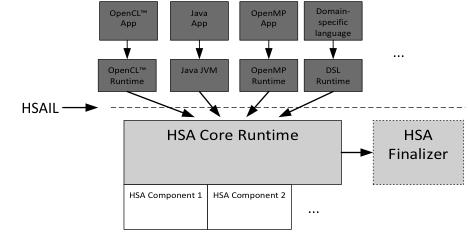
\includegraphics[width=0.5\textwidth]{fig/swarch}
  \centering
  \caption{HSA Software Architecture}
  \label{fig:swarch}
\end{figure}

Figure~\ref{fig:swarch} shows how the HSA Core Runtime fits into a
typical software architecture stack.

At the top of the stack is a programming model such as OpenCL™,
Java, OpenMP, or a domain-specific language (DSL).   The programming
model must include some way to indicate a parallel region that can
be accelerated.  For example, OpenCL has calls to
\texttt{clEnqueueNDRangeKernel} with associated kernels and grid ranges.
Java has the stream and lambda APIs, which provide support for both
multi-core CPUs and HSA Components.  OpenMP contains OMP pragmas
that mark parallel for loops and control other aspects of the
parallel implementation.  Other programming models can also build on
this same infrastructure.

The language compiler is responsible for generating HSAIL code for
the parallel regions.  HSA supports several options for when HSAIL
is generated and finalized.  One possibility is that the HSAIL is
generated by a high-level compiler and then embedded in the
application binary.  In this case, the finalizer is run when the
application loads and will convert the HSAIL to machine code for the
target machine.   Another option is that the HSAIL is finalized when
the applications is built, or the machine cod  The HSA Finalizer is
an optional component of the HSA Core Runtime, which may reduce the
footprint of the HSA software on systems where the finalization is
done before runtime.

Each language also includes a “language runtime” that connects the
language implementation to the HSA Core Runtime.   When the language
compiler generates code for a parallel region, it will include calls
to the HSA Runtime to set up and dispatch the work to the HSA
Component.   The language runtime is also responsible for
initializing HSA, and may utilize other HSA core runtime features as
well.

The API for the HSA core runtime is standard across all HSA vendors,
such that languages which use the HSA runtime can run on the
different vendors that support the API.  Each vendor is responsible
for supplying their own implementation which supports the hsa
component(s) in the vendor’s platform.   HSA does not provide a
mechanism to combine runtimes from different vendors; instead
vendors must provide a single runtime which supports all the
components in the platform.
The implementation of the HSA Runtime may include kernel-level
components (typical for hardware components) or may be entirely
user-space (simulators or CPU implementations).

\hypertarget{glue}{}\section{ Infrastructure and Execution
Flow}\label{glue}

\diffblock{
\hypertarget{executionmodel}{}\section{Execution
Model}\label{executionmodel}
}
\diffblock{\hypertarget{archdispatch}{}\subsection{Architected Dispatch}
\label{archdispatch}}
Core runtime exposes several details of the HSA hardware,
including architected dispatches and support for execution control.
The overall goal of the core runtime design is to provide a
high-\/performance dispatch mechanism that is portable across
multiple HSA vendor architectures. Two vendors with the same
host ISA but different HSA-\/compliant GPUs will be able
to run the same unmodified binary, because they support the
HSA-\/architected AQL interface and supply a library
that implements the architected core runtime API.

In order for user-level applications to use the HSA system and HSA
components, they need to write HSAIL programs and compile and
execute these programs using user mode queues and AQL commands.  The
HSA Programmer’s Reference Manual (PRM) defines HSAIL Virtual ISA
and Programming Model, serves as a Compiler Writer’s Guide, and
defines Object Format (BRIG). The HSA runtime helps setup the
execution via API calls and data structures to support architected
features.

The HSA core runtime realizes architected dispatch. Architected
dispatch is the key feature in an HSA system that enables a
user-\/level application to directly issue commands to the HSA
Component hardware.  Architected dispatch differentiates it from
other higher-\/level runtime systems and programming models\-: other
runtime systems provide software APIs for setting arguments and
launching kernels, while HSA architects these at the hardware
and specification level.  The critical path of the dispatch
mechanism is architected at the HSA hardware level and can be
done with regular memory operations and runtime provided wrapper
API.  Fundamentally, the user creates user mode queues and an
AQL Packet in memory, and then signals the HSA component to
begin executing the packet using light weight operations (which may
be wrapped with API calls).

This section describes various features core runtime provides to
support architected dispatch as steps that a user needs to take to
utilize runtime.

\subsection{Initial Setup}
One of the first steps in the setup is that of device discovery.
Device discovery is performed at the initialization of the core
runtime and information is made available to the user as data
structures. Section~\ref{topology} describes these structures.
The next step in the setup is creation of the
component queues. Queues are an HSA architected mechanism to submit
work to the HSA component HW. The interfaces for queue creation
are defined in Section~\ref{architected_queue}. Different
components may provide
implementation-\/specific code under the core API for these
functions. HSA runtime also includes mechanisms to provide
implementation-\/specific data as part of the dispatch, provided
such data can be computed at compile time.

\subsection{Compilation Flow}
Once an HSAIL program is written or generated by a higher-level
compilation step, it needs to be \emph{assembled} to generate a
BRIG. BRIG is the HSAIL object format and is specified in the PRM.
HSA runtime defines API call to compile the BRIG and generate a code
object that has sufficient information to execute the user
program. The details of this compilation process and symbol
resolution are discussed in Section~\ref{finalizerchapter}.

\subsection{Execution of Kernel}
The Systems Architecture Requirements (SAR) document specifies the
structure of the \emph{packets} (i.e. commands) that can be placed on
the HSA user mode queues for the component HW to execute them. The
format of the packets is architected and they are referred to as
Architected Queuing Language (AQL) packets. One of the types of AQL
packets is a dispatch AQL packet.
The user can now create an AQL packet
and initialize it with the code object obtained from the
finalization step, including the
allocation of memory to hold the kernel arguments and the
spill/arg/private memory.
The interface for kernel arguments between the runtime and the
kernel ISA (instruction set architecture) is also architected at
the HSA level. This is covered in the HSAIL ABI,
which specifies the in-\/memory layout of the kernarg segment. Users
can determine the layout of the kernarg memory segment at compile
time merely by examining the signature of the HSAIL
function. The finalizer is required to support this ABI and thus
there is no need for runtime metadata to specify the position or
format of arguments.
This step can be done once for each AQL packet creation.

Optimized implementations can cache the
result of this step and re-\/use the AQL packet for subsequent
launches. Care must be taken to ensure that the AQL Dispatch
packet (and the associated kernel and spill/arg/private memory) is
not re-\/used before the launch completes. For simple cases, (that
is, a single-\/thread, synchronous launch, the
AQL dispatch packet(s) can be declared as a static variable
and initialized at the same time the code is finalized. More
advanced cases can create and track several
AQL Dispatch packet(s) for a single kernel code object.

HSA HW defines a packet process for processing these packets and a doorbell
mechanism to inform the packet processing HW that packets have been
written into the queue. The Core runtime defines a structure and update
API to inform the HW that the dispatch packet has been written to the
queue. Different packet formats and states of a packet are discussed
in Section~\ref{AQL}. Section~\ref{architected_queue} discusses the
queue creation and various states the queue can be in, once it is
created.

Once the packet is written and the HW is informed by way of the
doorbell, the execution can start. The execution happens
asynchronously. The user is free to write more packets for executing
other kernels in the queue. This activity can overlap the actual
execution of the kernel.

\subsection{Determining Kernel Completion}
HSA SAR defines signals as a mechanism for communication between
different parts of a HSA system. Signals are defined as opaque
objects in the HSA core runtime and APIs have been defined to send a
value to the signal and wait for a value at the signal,
Section~\ref{signals} discusses signals in detail. The AQL dispatch
packet has a provision for the user to pass in an opaque signal.
When the HSA Component HW observes a valid signal in the AQL packet,
it sends a value to this signal when execution of the kernel is
complete (success or error). The user can wait on this signal to
determine kernel completion. Errors and their
meaning are discussed in Section~\ref{error}.
\lstinputlisting{example/main.c}

\chapter{HSA Core API Specification and Description} \label{coreapi}
\hypertarget{coreapi}{}
This chapter describes HSA Core runtime API by their functional
area. Note that except for any setter/getter API, the remainder of
the core runtime API may be considered thread-safe.  Both the signal
update and the queue index update API are setter/getter API and
define scope an synchronization that applies to the updates and
operate on structure elements.

Several operating systems allow functions to be executed when a DLL
or a shared library is loaded (e.g. DLL main in Windows and GCC
\emph{constructor/destructor} attributes that allow functions to be
executed prior to main in several operating systems).
Whether or not the HSA runtime functions are allowed to be invoked
in such fashion may be implementation specific and are outside the
scope of this specification.

Similarly, any header files distributed by the HSA foundation for
this spec may contain calling convention specific prefixes such as
\_\_cdecl or \_\_stdcall. Such calling conventions are again invocation,
usage and implementation specific. Hence, the calling convention
specific prefix definition is outside the scope of API definition.

\begin{DIFnomarkup}
\hypertarget{error}{}\section{Errors and Notifications}
\label{error}
\end{DIFnomarkup}

Error handling in the core runtime can broadly be classified into
two categories: synchronous error handling and asynchronous
error/notification handling.

Synchronous errors are always reported when the call returns. They
indicate if the API returned a success or an error.

Asynchronous errors can occur due to various reasons:
\begin{inparaenum}[(i)]

\item Activity in packet processor, executing kernels, their actions
and memory accesses. If an error is detected during execution of a
kernel, the completion signal (if present) will be signaled with an
error indication value.

\item To provide \emphld{information/warning} (not as an exception
in expected behavior but by definition). This information/warning
may not necessarily indicate an error. For example, a timeout may be
an acceptable response for a wait API but is not indicative of a
failure.

\end{inparaenum}

\begin{DIFnomarkup}
\hypertarget{syncerror}{}\subsection{Synchronous Errors }\label{syncerror}
\end{DIFnomarkup}

When a core runtime API is called by the user and does not execute
successfully, the core runtime returns a status that can help
determine a cause of the unsuccessful execution. Each API call
discussed in this chapter defines what constitutes a successful
execution. While a few error conditions can be generalized to a
certain degree (e.g. failure in allocating system memory) many
errors can have system/implementation specific explanations.

The HSA core runtime API defines an enumeration that captures the
result of any API function that has been executed (the only
exception to this behavior are setter/getter API that access core
runtime structures). This enumeration is of the type
\reftyp{hsa\_status\_t} and enumerates \emphld{success},
\emphld{info}, and \emphld{error}. The \emphld{info} status definition
is discussed in Section ~\ref{asyncerror}.

\vspace{3mm}\emphld{Success} status is a single constant,
\refenu{HSA\_STATUS\_SUCCESS}, with value 0. Description of every core
runtime API call that returns \reftyp{hsa\_status\_t} explains the
expected successful behavior for that API.

\emphld{Error} status could be due to user input/actions that are not
allowed (e.g. negative value in a size for allocation) or systemic
errors (e.g. an asynchronous activity lead to a failure that
cascaded into a failure in this API). The constants used for error
status are restricted to the negative range of values within the
\reftyp{hsa\_status\_t} enumeration. Errors must always have a
negative value. The Name of any constant that indicates an error status is
prefixed by \refenu{HSA\_STATUS\_ERROR}. Errors could potentially be
implementation.

While the name of the constant in itself is informative for success,
info or error status, there may be scenarios where
\begin{inparaenum}[(i)] \item the user may request more information
about the meaning of a particular status, or, \item the return
status was implementation specific and the user needs to decode it.
\end{inparaenum} In the case of implementation specific status, the
negative number returned for error may not correspond to a
particular enumeration constant. To query additional
information on synchronous errors, the core runtime defines the
following API:

\makeatletter{}

\noindent\begin{tcolorbox}[breakable,nobeforeafter,colframe=white,colback=lightgray,left=0mm]
\hsatyp{group__status_1gad755322e7ff95456520e8abdbe90d225}{hsa\_status\_t} \hsadef{group__status__query_1gaf3032aa83b93991d945e572fce1f8fec}{hsa\_status\_query\_description}(
\vspace{-3.5mm}\begin{longtable}{@{}p{\textwidth}}
\hspace{1.7em}\hsatyp{group__status_1gad755322e7ff95456520e8abdbe90d225}{hsa\_status\_t} \hsaarg{input\_status},\\
\hspace{1.7em}uint64\_t * \hsaarg{status\_info},\\
\hspace{1.7em}char *const * \hsaarg{status\_info\_string})\end{longtable}

\end{tcolorbox}
Queries additional information on synchronous errors.

\noindent\textbf{Parameters}\\[-6mm]
\noindent\begin{longtable}{@{}>{\hangindent=2em}p{\textwidth}}
\hsaarg{input\_status}\\\hspace{2em}(in) Any unsuccessful API return status that the user is seeking more information on.\\[2mm]
\hsaarg{status\_info}\\\hspace{2em}(in) User allocated. In addition to the string. This value could be 0 and in itself (without \hsaarg{status\_info\_string}) may not be independently interpretable by the user.\\[2mm]
\hsaarg{status\_info\_string}\\\hspace{2em}(out) A ISO/IEC 646 encoded english language string that potentially describes the error status. The string terminates in a ISO 646 defined NUL char.
\end{longtable}
\vspace{-5mm}\noindent\textbf{Return Values}\\[-6mm]
\noindent\begin{longtable}{@{}>{\hangindent=2em}p{\linewidth}}
\hsatyp{group__status_1ggad755322e7ff95456520e8abdbe90d225ae382ea0c9c05cce5a60d0317375159cc}{HSA\_STATUS\_SUCCESS}\\\hspace{2em}If successful\\[2mm]
\hsatyp{group__status_1ggad755322e7ff95456520e8abdbe90d225ac7d3651f75107d2a6a8ba3b25683c030}{HSA\_STATUS\_ERROR\_INVALID\_ARGUMENT}\\\hspace{2em}If a NULL value is passed for either of the arguments
\end{longtable}
\vspace{-4mm}\noindent\textbf{Description}\\[1mm]
Returns success if one or both of the \hsaarg{status\_info} and \hsaarg{status\_info\_string} have been successfully updated with information regarding the input \hsaarg{input\_status}. 
 

\begin{DIFnomarkup}
\hypertarget{asyncerror}{}\subsection{Asynchronous Errors and
Notifications}\label{asyncerror}
\end{DIFnomarkup}

The HSA core runtime supports user-defined callbacks to handle
asynchronous errors. There are two different categories of callbacks
that can be registered by the user: \begin{inparaenum}[(i)] \item
for asynchronous information or warnings generated when the runtime
is executing, or, \item for asynchronous errors that get generated
in packet processor, or while executing a kernel \end{inparaenum}.
The core runtime supports a callback each for asynchronous errors
and notifications.
The user must use caution when using blocking functions within their
callback implementation -- a callback that does not return can
render the runtime state to be undefined. The user cannot depend on
thread local storage within the callbacks implementation and may
safely kill the thread that registers the callback. It is the user's
responsibility to ensure that the callback function is thread-safe.
The runtime does not implement any default callbacks.

\subsubsection{Asynchronous Notification of Information or
Warning}\label{asynnotif}
The information/warning status is represented by a value greater
than 0 within the \reftyp{hsa\_status\_t} enumeration. The status is
up to user interpretation and the runtime allows the user to
register a callback to take necessary action. Consider the example
where a user calls the initialize API to initialize the core runtime
and the return status is
\refenu{HSA\_STATUS\_INFO\_ALREADY\_INITIALIZED} (to indicate that
the core runtime has already been initialized). This result may be
interpreted differently in different usage scenarios. A callback for
such notifications may be registered via \reffun{hsa\_open} API
discussed in Section~\ref{init} or via
\reffun{hsa\_notification\_callback\_register} API, which is defined
as follows:

\makeatletter{}

\noindent\begin{tcolorbox}[breakable,nobeforeafter,colframe=white,colback=lightgray,left=0mm]
\hsatyp{group__status_1gad755322e7ff95456520e8abdbe90d225}{hsa\_status\_t} \hsadef{group__register__notify_1ga689986418b308574a7688d674e65350e}{hsa\_notification\_callback\_register}(
\vspace{-3.5mm}\begin{longtable}{@{}p{\textwidth}}
\hspace{1.7em}void(*)(const \hsatyp{group__notify__message_1ga46fc2648e5bde0dfc932de4acb246d82}{hsa\_notification\_info\_t} *info) \hsaarg{notification\_callback},\\
\hspace{1.7em}void * \hsaarg{user\_data},\\
\hspace{1.7em}\hsatyp{group__runtime__context_1ga0296b674c03f1a65fa8ef91e2f0ad44d}{hsa\_runtime\_context\_t} * \hsaarg{context})\end{longtable}

\end{tcolorbox}
Register a notification callback.

\noindent\textbf{Parameters}\\[-6mm]
\noindent\begin{longtable}{@{}>{\hangindent=2em}p{\textwidth}}
\hsaarg{notification\_callback}\\\hspace{2em}(in) The callback that the user is registering, the callback is called with info as a parameter. User can read the structure and access its elements.\\[2mm]
\hsaarg{user\_data}\\\hspace{2em}(in) The user data to call the callback with. info.user\_data will be filled with value when the callback is called.\\[2mm]
\hsaarg{context}\\\hspace{2em}(in) Identifies a particular runtime context that this callback is registered for. When a callback is registered for a particular context, it will only be invoked if the notification is for an action in that context.
\end{longtable}
\vspace{-5mm}\noindent\textbf{Return Values}\\[-6mm]
\noindent\begin{longtable}{@{}>{\hangindent=2em}p{\linewidth}}
\hsatyp{group__status_1ggad755322e7ff95456520e8abdbe90d225ae382ea0c9c05cce5a60d0317375159cc}{HSA\_STATUS\_SUCCESS}\\\hspace{2em}If successful\\[2mm]
\hsatyp{group__status_1ggad755322e7ff95456520e8abdbe90d225a1a77fcf36d0d140874c4361ab093eff7}{HSA\_STATUS\_ERROR\_OUT\_OF\_RESOURCES}\\\hspace{2em}If there is a failure in allocation of an internal structure required by the core runtime library in the context of registering a callback. This error may also occur when the core runtime library needs to spawn threads or create internal OS-specific events.\\[2mm]
\hsatyp{group__status_1ggad755322e7ff95456520e8abdbe90d225ac7d3651f75107d2a6a8ba3b25683c030}{HSA\_STATUS\_ERROR\_INVALID\_ARGUMENT}\\\hspace{2em}If \hsaarg{info} is NULL.\\[2mm]
\hsatyp{group__status_1ggad755322e7ff95456520e8abdbe90d225a7bd6aaae8ecaaaea4c0d12e406e13b53}{HSA\_STATUS\_ERROR\_INVALID\_CONTEXT}\\\hspace{2em}If the context is invalid (e.g. referenced counted to 0).
\end{longtable}
 
 

One of the arguments of the notification callback is a structure
that contains notification information. The structure is defined as
follows:

\makeatletter{}

\noindent\begin{tcolorbox}[breakable,nobeforeafter,arc=0mm,colframe=white,colback=lightgray,left=0mm]
struct \hsadef{group__notify__message_1ga46fc2648e5bde0dfc932de4acb246d82}{hsa\_notification\_info\_t}
\vspace{-3.5mm}\begin{longtable}{@{}p{\textwidth}}
\hspace{1.7em}\hsatyp{group__status_1gad755322e7ff95456520e8abdbe90d225}{hsa\_status\_t} \hsaarg{status}\\
\hspace{1.7em}void * \hsaarg{ptr\_info}\\
\hspace{1.7em}char * \hsaarg{string\_info}\\
\hspace{1.7em}void * \hsaarg{user\_data}
\end{longtable}

\end{tcolorbox}
Notification information.

\noindent\textbf{Data Fields}\\[-5mm]
\begin{longtable}{@{}>{\hangindent=2em}p{\textwidth}}
\hsaarg{status}\\\hspace{2em}The info status enum value.\\[2mm]
\hsaarg{ptr\_info}\\\hspace{2em}A pointer to more information, this could be pointing to implementation specific details that could be useful to some tools or to binary data.\\[2mm]
\hsaarg{string\_info}\\\hspace{2em}ISO/IEC 646 character encoding must be used. A string indicating some error information. The string should be NUL terminated per ISO 646.\\[2mm]
\hsaarg{user\_data}\\\hspace{2em}A pointer to user supplied data.
\end{longtable}

 

\subsubsection{Asynchronous Notification of Errors}\label{asynnotif}

The HSA system can have several queues in operation and
several kernels executing from these queues asynchronously.
When any asynchronous activity generates an error, the action that
initiated the activity may have concluded. To deal with
asynchronous errors, the core runtime supports asynchronous error
callbacks. The asynchronous error callback may be registered by means of the
\reffun{hsa\_open} API discussed in Section~\ref{init} or via
\reffun{hsa\_error\_callback\_register} API, which is defined as
follows:

\makeatletter{}

\noindent\begin{tcolorbox}[breakable,nobeforeafter,colframe=white,colback=lightgray,left=0mm]
\hsatyp{group__status_1gad755322e7ff95456520e8abdbe90d225}{hsa\_status\_t} \hsadef{group__register__error_1ga5822750cf61973dace0f68013c4cd52c}{hsa\_error\_callback\_register}(
\vspace{-3.5mm}\begin{longtable}{@{}p{\textwidth}}
\hspace{1.7em}void(*)(const \hsatyp{group__error__message_1ga1e98022fc32cd651dc83c5f871e1a960}{hsa\_async\_error\_info\_t} *info) \hsaarg{error\_callback},\\
\hspace{1.7em}void * \hsaarg{user\_data},\\
\hspace{1.7em}\hsatyp{group__runtime__context_1ga0296b674c03f1a65fa8ef91e2f0ad44d}{hsa\_runtime\_context\_t} * \hsaarg{context})\end{longtable}

\end{tcolorbox}
Register an error callback.

\noindent\textbf{Parameters}\\[-6mm]
\noindent\begin{longtable}{@{}>{\hangindent=2em}p{\textwidth}}
\hsaarg{error\_callback}\\\hspace{2em}(in) The callback that the user is registering, the callback is called with info structure. User can read the structure and access its elements.\\[2mm]
\hsaarg{user\_data}\\\hspace{2em}(in) The user data to call the callback with. info.user\_data will be filled with value when the callback is called.\\[2mm]
\hsaarg{context}\\\hspace{2em}(in) The runtime context that this callback is being registered for.
\end{longtable}
\vspace{-5mm}\noindent\textbf{Return Values}\\[-6mm]
\noindent\begin{longtable}{@{}>{\hangindent=2em}p{\linewidth}}
\hsatyp{group__status_1ggad755322e7ff95456520e8abdbe90d225ae382ea0c9c05cce5a60d0317375159cc}{HSA\_STATUS\_SUCCESS}\\\hspace{2em}If successful\\[2mm]
\hsatyp{group__status_1ggad755322e7ff95456520e8abdbe90d225a1a77fcf36d0d140874c4361ab093eff7}{HSA\_STATUS\_ERROR\_OUT\_OF\_RESOURCES}\\\hspace{2em}If there is a failure in allocation of an internal structure required by the core runtime library in the context of registering a callback. This error may also occur when the core runtime library needs to spawn threads or create internal OS-specific events.\\[2mm]
\hsatyp{group__status_1ggad755322e7ff95456520e8abdbe90d225ac7d3651f75107d2a6a8ba3b25683c030}{HSA\_STATUS\_ERROR\_INVALID\_ARGUMENT}\\\hspace{2em}If \hsaarg{info} is NULL.
\end{longtable}
\vspace{-4mm}\noindent\textbf{Description}\\[1mm]
When a callback is registered for a particular context, it will only be invoked if the notification is for an action in that context. For example, if a queue was created for a runtime context \hsaarg{c1} and a callback registered for a context \hsaarg{c2} but not for \hsaarg{c1}, any error on the queue, such as a packet processing error, will not trigger the execution of asynchronous error callback registered for context \hsaarg{c1}. 
 

Details on how association of the callback can be done with
asynchronous activities are discussed in Sections~\ref{init} and
\ref{architected_queue}.

One of the arguments of the notification callback is a structure
that contains notification information. The structure is defined as
follows:

\makeatletter{}

\noindent\begin{tcolorbox}[breakable,nobeforeafter,arc=0mm,colframe=white,colback=lightgray,left=0mm]
struct \hsadef{group__error__message_1ga1e98022fc32cd651dc83c5f871e1a960}{hsa\_async\_error\_info\_t}
\vspace{-3.5mm}\begin{longtable}{@{}p{\textwidth}}
\hspace{1.7em}\hsatyp{group__status_1gad755322e7ff95456520e8abdbe90d225}{hsa\_status\_t} \hsaarg{error\_type}\\
\hspace{1.7em}uint32\_t \hsaarg{queue\_id}\\
\hspace{1.7em}void * \hsaarg{ptr\_info}\\
\hspace{1.7em}char * \hsaarg{string\_info}\\
\hspace{1.7em}void * \hsaarg{user\_data}\\
\hspace{1.7em}uint64\_t \hsaarg{timestamp}\\
\hspace{1.7em}uint64\_t \hsaarg{reserved1}\\
\hspace{1.7em}uint64\_t \hsaarg{reserved2}\\
\hspace{1.7em}uint64\_t \hsaarg{reserved3}
\end{longtable}

\end{tcolorbox}
TODO.

\noindent\textbf{Data Fields}\\[-5mm]
\begin{longtable}{@{}>{\hangindent=2em}p{\textwidth}}
\hsaarg{error\_type}\\\hspace{2em}Indicates the type of the error, based on this, the user knows if and packet\_id is available in one of the reserved words.\\[2mm]
\hsaarg{queue\_id}\\\hspace{2em}The queue that processed the entity that caused the asynchronous error.\\[2mm]
\hsaarg{ptr\_info}\\\hspace{2em}A pointer to more information, this could be pointing to implementation specific details that could be useful to some tools or to binary data\\[2mm]
\hsaarg{string\_info}\\\hspace{2em}ISO/IEC 646 character encoding must be used. A string indicating some error information. The string should be NUL terminated per ISO 646.\\[2mm]
\hsaarg{user\_data}\\\hspace{2em}A pointer to user supplied data\\[2mm]
\hsaarg{timestamp}\\\hspace{2em}System timestamp to indicate when the error was discovered, the implementation may chose to always return 0 and user must take it into account when utilizing the timestamp.\\[2mm]
\hsaarg{reserved1}\\\hspace{2em}Additional info to be intepreted based on \hsaarg{error\_type}.\\[2mm]
\hsaarg{reserved2}\\\hspace{2em}Additional info to be intepreted based on \hsaarg{error\_type}.\\[2mm]
\hsaarg{reserved3}\\\hspace{2em}Additional info to be intepreted based on \hsaarg{error\_type}.
\end{longtable}

 

\subsection{Asynchronous Notification Example}
\lstinputlisting{example/asyncerror.c}


\hypertarget{init}{}\section{Open and close}\label{init}

Since HSA core runtime is a user mode library, its state is a part
of the application's process space. When the runtime is opened for
the first time, a runtime instance for that application process is
created. Closing a runtime destroys this instance. An application
may open (or close) the HSA runtime multiple times within the same
process and potentially within multiple threads -- only a
single instance of the runtime, per-process, will exist.

The core runtime defines a runtime context that acts as a reference
counting mechanism and a scheme to differentiate multiple usages of
the runtime within the same application process. The runtime context
is generated when the runtime is opened or when a
user calls the acquire API that is defined in this Section. As an
example, consider an application that is using the runtime but also
uses a library, this library also creates HSA queues and submits
work to them. Both the library and the application may want to register
callbacks, and to capture notifications/errors of their specific
usage. The runtime context helps identify the different usages (within
the same process) and channel errors and notifications to
appropriate callbacks. It also acts as a reference counting
mechanism; while correctly \emphld{acquired}, the runtime context
ensures that the runtime instance will not be shutdown until the
context is \emphld{released} (this, in effect, is the reference
counting part of the context).

This section defines four new APIs to open (\reffun{hsa\_open}) a
runtime instance, close it (\reffun{hsa\_close}), create a new context
(\reffun{hsa\_context\_acquire}) and release the acquired
context(\reffun{hsa\_context\_release}.

\makeatletter{}

\noindent\begin{tcolorbox}[breakable,nobeforeafter,colframe=white,colback=lightgray,left=0mm]
\hsatyp{group__status_1gad755322e7ff95456520e8abdbe90d225}{hsa\_status\_t} \hsadef{group__openclose_1gab45607a30ab05c95dfe692115fe1f2a4}{hsa\_open}(
\vspace{-3.5mm}\begin{longtable}{@{}p{\textwidth}}
\hspace{1.7em}\hsatyp{group__runtime__context_1ga0296b674c03f1a65fa8ef91e2f0ad44d}{hsa\_runtime\_context\_t} ** \hsaarg{context})\end{longtable}

\end{tcolorbox}
Initialize the HSA runtime.

\noindent\textbf{Parameters}\\[-6mm]
\noindent\begin{longtable}{@{}>{\hangindent=2em}p{\textwidth}}
\hsaarg{context}\\\hspace{2em}(out) A type for reference counting. User allocated.
\end{longtable}
\vspace{-5mm}\noindent\textbf{Return Values}\\[-6mm]
\noindent\begin{longtable}{@{}>{\hangindent=2em}p{\linewidth}}
\hsatyp{group__status_1ggad755322e7ff95456520e8abdbe90d225ae382ea0c9c05cce5a60d0317375159cc}{HSA\_STATUS\_SUCCESS}\\\hspace{2em}If successful.\\[2mm]
\hsatyp{group__status_1ggad755322e7ff95456520e8abdbe90d225a1a77fcf36d0d140874c4361ab093eff7}{HSA\_STATUS\_ERROR\_OUT\_OF\_RESOURCES}\\\hspace{2em}if there is a failure in allocation of an internal structure required by the core runtime library. This error may also occur when the core runtime library needs to spawn threads or create internal OS-specific events.\\[2mm]
\hsatyp{group__status_1ggad755322e7ff95456520e8abdbe90d225ac2b1926b00231fd6a7695c1470c43ef6}{HSA\_STATUS\_ERROR\_COMPONENT\_INITIALIZATION}\\\hspace{2em}If there is a non-specific failure in initializing one of the components.\\[2mm]
\hsatyp{group__status_1ggad755322e7ff95456520e8abdbe90d225a2ae9f2db427b200c2709bac49f4cabfb}{HSA\_STATUS\_ERROR\_CONTEXT\_NULL}\\\hspace{2em}If the context pointer passed by the user is NULL. User is required to pass in a memory backed context pointer.
\end{longtable}
\vspace{-4mm}\noindent\textbf{Description}\\[1mm]
Initializes the HSA runtime if it is not already initialized. It is allowed for applications to invoke \hsatyp{group__openclose_1gab45607a30ab05c95dfe692115fe1f2a4}{hsa\_open} multiple times. The HSA open call returns a new context at every invocation. Reference counting is a mechanism that allows the runtime to keep a count of the number of different usages of the runtime API within the same application process. This ensures that the runtime stays active until \hsatyp{group__openclose_1gae008f9f4f2d3939b2ccd1c378b8cc4f0}{hsa\_close} is called by the user when the reference count represented by that runtime context is one.\\[2mm]
If the HSA runtime is already initialized, an asynchronous notification is generated by the runtime and \hsatyp{group__status_1ggad755322e7ff95456520e8abdbe90d225ae382ea0c9c05cce5a60d0317375159cc}{HSA\_STATUS\_SUCCESS} is returned. If the user chooses to capture this asynchronous notification, the user should define a callback and associate it with the context returned by the \hsatyp{group__openclose_1gab45607a30ab05c95dfe692115fe1f2a4}{hsa\_open} call. Each open call increments the reference count before returning success. 


\noindent\begin{tcolorbox}[breakable,nobeforeafter,colframe=white,colback=lightgray,left=0mm]
\hsatyp{group__status_1gad755322e7ff95456520e8abdbe90d225}{hsa\_status\_t} \hsadef{group__openclose_1gae008f9f4f2d3939b2ccd1c378b8cc4f0}{hsa\_close}(
\vspace{-3.5mm}\begin{longtable}{@{}p{\textwidth}}
\hspace{1.7em}\hsatyp{group__runtime__context_1ga0296b674c03f1a65fa8ef91e2f0ad44d}{hsa\_runtime\_context\_t} * \hsaarg{context})\end{longtable}

\end{tcolorbox}
Close the HSA runtime.

\noindent\textbf{Parameters}\\[-6mm]
\noindent\begin{longtable}{@{}>{\hangindent=2em}p{\textwidth}}
\hsaarg{context}\\\hspace{2em}(in) Context to close.
\end{longtable}
\vspace{-5mm}\noindent\textbf{Return Values}\\[-6mm]
\noindent\begin{longtable}{@{}>{\hangindent=2em}p{\linewidth}}
\hsatyp{group__status_1ggad755322e7ff95456520e8abdbe90d225ae382ea0c9c05cce5a60d0317375159cc}{HSA\_STATUS\_SUCCESS}\\\hspace{2em}If successful.\\[2mm]
\hsatyp{group__status_1ggad755322e7ff95456520e8abdbe90d225a34ea59ade5bfce95eee935238a99f5b5}{HSA\_STATUS\_ERROR\_NOT\_INITIALIZED}\\\hspace{2em}If invoked before the runtime was initialized, or after it has already been successfully closed.\\[2mm]
\hsatyp{group__status_1ggad755322e7ff95456520e8abdbe90d225a6406af88203fcbec4179fbb71cc66b65}{HSA\_STATUS\_ERROR\_RESOURCE\_FREE}\\\hspace{2em}If some of the resources consumed during initialization by the runtime could not be freed.
\end{longtable}
\vspace{-4mm}\noindent\textbf{Description}\\[1mm]
Decreases the context reference count for every invocation. Once the reference count is zero, it proceeds to relinquish any resources allocated for the runtime and closes the runtime instance. It is possible in a multi-threaded scenario that one thread is doing a close while the other is trying to acquire the runtime context or do an open. The core runtime specification defines that an acquire with an input context that represents a closed runtime instance will fail. However, \hsatyp{group__openclose_1gab45607a30ab05c95dfe692115fe1f2a4}{hsa\_open} can be called to create a new instance of the runtime after it is closed.\\[2mm]
An invocation when the reference count is not one it is considered succesful in that \hsatyp{group__status_1ggad755322e7ff95456520e8abdbe90d225ae382ea0c9c05cce5a60d0317375159cc}{HSA\_STATUS\_SUCCESS} is returned with status \hsatyp{group__status_1ggad755322e7ff95456520e8abdbe90d225ae2924e022da18c1062e3b418a5bab43c}{HSA\_STATUS\_CLOSE\_CONTEXT\_ACTIVE}, is generated by the runtime on the context that is still active before the API returns. 


\noindent\begin{tcolorbox}[breakable,nobeforeafter,colframe=white,colback=lightgray,left=0mm]
\hsatyp{group__status_1gad755322e7ff95456520e8abdbe90d225}{hsa\_status\_t} \hsadef{group__openclose_1gac10422c957e78aa183b830495c20cd25}{hsa\_context\_acquire}(
\vspace{-3.5mm}\begin{longtable}{@{}p{\textwidth}}
\hspace{1.7em}\hsatyp{group__runtime__context_1ga0296b674c03f1a65fa8ef91e2f0ad44d}{hsa\_runtime\_context\_t} * \hsaarg{input\_context})\end{longtable}

\end{tcolorbox}
Increment reference count of a context.

\noindent\textbf{Parameters}\\[-6mm]
\noindent\begin{longtable}{@{}>{\hangindent=2em}p{\textwidth}}
\hsaarg{input\_context}\\\hspace{2em}(in) The context that the user is explicitely reference counting, increment reference count if not 0. User allocated.
\end{longtable}
\vspace{-5mm}\noindent\textbf{Return Values}\\[-6mm]
\noindent\begin{longtable}{@{}>{\hangindent=2em}p{\linewidth}}
\hsatyp{group__status_1ggad755322e7ff95456520e8abdbe90d225ae382ea0c9c05cce5a60d0317375159cc}{HSA\_STATUS\_SUCCESS}\\\hspace{2em}If successful.\\[2mm]
\hsatyp{group__status_1ggad755322e7ff95456520e8abdbe90d225a34ea59ade5bfce95eee935238a99f5b5}{HSA\_STATUS\_ERROR\_NOT\_INITIALIZED}\\\hspace{2em}If invoked before the runtime was initialized or after it has been closed.\\[2mm]
\hsatyp{group__status_1ggad755322e7ff95456520e8abdbe90d225a342227d93a263cefbacb5cde75fa386f}{HSA\_STATUS\_CONTEXT\_LIMIT\_REACHED}\\\hspace{2em}If the reference count has reached UINT64\_MAX
\end{longtable}
 


\noindent\begin{tcolorbox}[breakable,nobeforeafter,colframe=white,colback=lightgray,left=0mm]
\hsatyp{group__status_1gad755322e7ff95456520e8abdbe90d225}{hsa\_status\_t} \hsadef{group__openclose_1ga9e080a819a1114577ccb53cc7f767470}{hsa\_context\_release}(
\vspace{-3.5mm}\begin{longtable}{@{}p{\textwidth}}
\hspace{1.7em}\hsatyp{group__runtime__context_1ga0296b674c03f1a65fa8ef91e2f0ad44d}{hsa\_runtime\_context\_t} * \hsaarg{input\_context})\end{longtable}

\end{tcolorbox}
Decrement reference count of a context.

\noindent\textbf{Parameters}\\[-6mm]
\noindent\begin{longtable}{@{}>{\hangindent=2em}p{\textwidth}}
\hsaarg{input\_context}\\\hspace{2em}(in) The context that the user is explicitely reference counting, decrement reference count if not 1. User allocated.
\end{longtable}
\vspace{-5mm}\noindent\textbf{Return Values}\\[-6mm]
\noindent\begin{longtable}{@{}>{\hangindent=2em}p{\linewidth}}
\hsatyp{group__status_1ggad755322e7ff95456520e8abdbe90d225ae382ea0c9c05cce5a60d0317375159cc}{HSA\_STATUS\_SUCCESS}\\\hspace{2em}If successful.\\[2mm]
\hsatyp{group__status_1ggad755322e7ff95456520e8abdbe90d225a34ea59ade5bfce95eee935238a99f5b5}{HSA\_STATUS\_ERROR\_NOT\_INITIALIZED}\\\hspace{2em}If invoked before the runtime was initialized or when the reference count is already zero.
\end{longtable}
 
 

\subsection{Example}
\lstinputlisting{example/openclose.c}

 \hypertarget{component}{}\section{Topology and Component
}\label{topology} HSA platform topology information is provided by the
runtime by way of data structures so user can gather details about how
a HSA system/platform exposed its architectural details such as agents
and memory. This information could be utilized by the user in
different ways including decisions on where to execute a particular
user task. Core runtime specification defines the topology table data
structure and other data structures to represent topology hierarchy.
After the core runtime is initialized with \reffun{hsa\_open}, the user
may create a local copy of the topology information using the API
\reffun{hsa\_topology\_table\_create}. The user can parse this table
representing the HSA system to gather details such as the number of
different HSA Components on the system with local access to a
particular set of memory resources. The topology table is designed to
be allocated in a block of contiguous memory.

\makeatletter{}

\noindent\begin{tcolorbox}[breakable,nobeforeafter,colframe=white,colback=lightgray,left=0mm]
\hsatyp{group__status_1gad755322e7ff95456520e8abdbe90d225}{hsa\_status\_t} \hsadef{group__topology__create_1ga22a5c0a0f393b8155a8791c4e5cc8486}{hsa\_topology\_table\_create}(
\vspace{-3.5mm}\begin{longtable}{@{}p{\textwidth}}
\hspace{1.7em}\hsatyp{group__topology__header_1gac319dcc24a76b155d6d5265dcc0cf453}{hsa\_topology\_header\_t} ** \hsaarg{header})\end{longtable}

\end{tcolorbox}
Retrieve topology information.

\noindent\textbf{Parameters}\\[-6mm]
\noindent\begin{longtable}{@{}>{\hangindent=2em}p{\textwidth}}
\hsaarg{header}\\\hspace{2em}(out) The topology header, this includes the base pointers to the rest of the topology table. Runtime allocated.
\end{longtable}
\vspace{-5mm}\noindent\textbf{Return Values}\\[-6mm]
\noindent\begin{longtable}{@{}>{\hangindent=2em}p{\linewidth}}
\hsatyp{group__status_1ggad755322e7ff95456520e8abdbe90d225ae382ea0c9c05cce5a60d0317375159cc}{HSA\_STATUS\_SUCCESS}\\\hspace{2em}If successful.\\[2mm]
\hsatyp{group__status_1ggad755322e7ff95456520e8abdbe90d225ac7d3651f75107d2a6a8ba3b25683c030}{HSA\_STATUS\_ERROR\_INVALID\_ARGUMENT}\\\hspace{2em}If \hsaarg{header} is NULL.\\[2mm]
\hsatyp{group__status_1ggad755322e7ff95456520e8abdbe90d225a1a77fcf36d0d140874c4361ab093eff7}{HSA\_STATUS\_ERROR\_OUT\_OF\_RESOURCES}\\\hspace{2em}If there is a failure in allocation of an internal structure required by the core runtime or in the creation of table header or the actual table.
\end{longtable}
 
 

\begin{figure}[b]
  \centering
  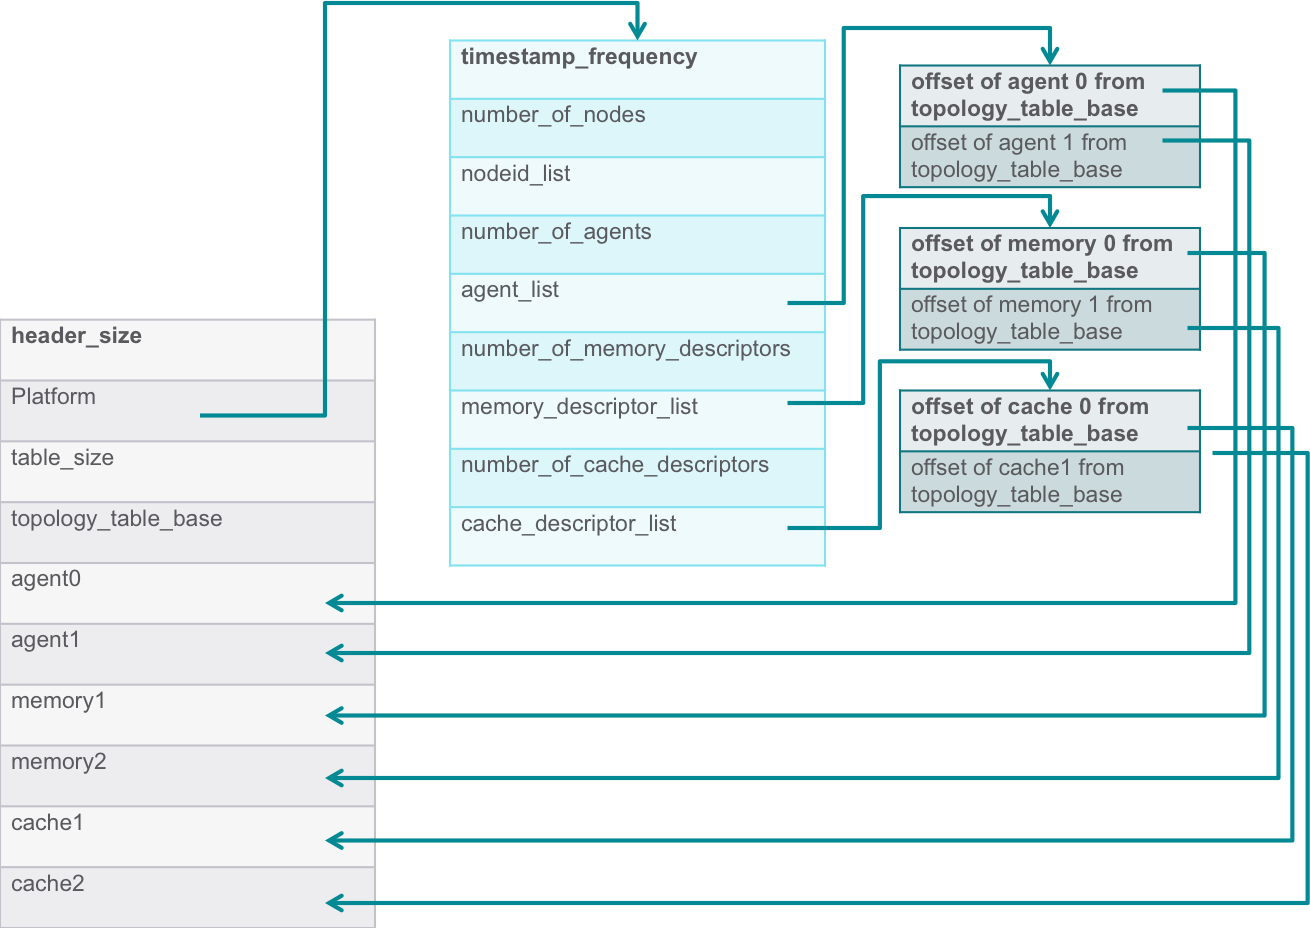
\includegraphics[width=0.5\textwidth]{fig/topologytable}
  \centering
  \caption{Structure of the Topology Table}
  \label{fig:topology_table}
\end{figure}

The table structure is shown in Figure~\ref{fig:topology_table}.
The first entity in the table is a table header. This is the output
of the \reffun{hsa\_topology\_table\_create} API, and is defined as:
\makeatletter{}

\noindent\begin{tcolorbox}[breakable,nobeforeafter,arc=0mm,colframe=white,colback=lightgray,left=0mm]
struct \hsadef{group__topology__header_1gac319dcc24a76b155d6d5265dcc0cf453}{hsa\_topology\_header\_t}
\vspace{-3.5mm}\begin{longtable}{@{}p{\textwidth}}
\hspace{1.7em}uint32\_t \hsaarg{header\_size\_bytes}\\
\hspace{1.7em}\hsatyp{group__platform_1gac15087b44d735fd1479fc754de556a00}{hsa\_platform\_t} \hsaarg{platform}\\
\hspace{1.7em}uint32\_t \hsaarg{table\_size}\\
\hspace{1.7em}void * \hsaarg{topology\_table\_base}
\end{longtable}

\end{tcolorbox}
Topology header.

\noindent\textbf{Data Fields}\\[-5mm]
\begin{longtable}{@{}>{\hangindent=2em}p{\textwidth}}
\hsaarg{header\_size\_bytes}\\\hspace{2em}Size of the header.\\[2mm]
\hsaarg{platform}\\\hspace{2em}The hierarchical platform structure that abstracts the table.\\[2mm]
\hsaarg{table\_size}\\\hspace{2em}Size of the table.\\[2mm]
\hsaarg{topology\_table\_base}\\\hspace{2em}Table base address, points to the table which starts with \hsatyp{group__platform_1gac15087b44d735fd1479fc754de556a00}{hsa\_platform\_t} structure
\end{longtable}

 

The table header structure includes the platform structure (
\reftyp{hsa\_platform\_t}), defined below.  The platform information in
the platform structure includes size/offset-array pairs for HSA agents
(\reftyp{hsa\_agent\_t}), memory (\reftyp{hsa\_memory\_descriptor\_t}) and
cache (\reftyp{hsa\_cache\_descriptor\_t}).  HSA platform can have a
hierarchical structure with multiple components/agents and physical
memories.  The \reftyp{hsa\_platform\_t} structure also includes
properties such as the clock frequency that are common across the
platform and also links to various elements in the topology table (see
Figure \ref{fig:topology_table}).

\makeatletter{}

\noindent\begin{tcolorbox}[breakable,nobeforeafter,arc=0mm,colframe=white,colback=lightgray,left=0mm]
struct \hsadef{group__platform_1gac15087b44d735fd1479fc754de556a00}{hsa\_platform\_t}
\vspace{-3.5mm}\begin{longtable}{@{}p{\textwidth}}
\hspace{1.7em}uint32\_t \hsaarg{hsa\_system\_timestamp\_frequency\_mhz}\\
\hspace{1.7em}uint8\_t \hsaarg{number\_of\_nodes}\\
\hspace{1.7em}uint32\_t * \hsaarg{node\_id}\\
\hspace{1.7em}uint32\_t \hsaarg{number\_of\_agents}\\
\hspace{1.7em}uint32\_t * \hsaarg{agent\_offset\_list\_bytes}\\
\hspace{1.7em}uint32\_t \hsaarg{number\_memory\_descriptors}\\
\hspace{1.7em}uint32\_t * \hsaarg{memory\_descriptor\_offset\_list\_bytes}\\
\hspace{1.7em}uint32\_t \hsaarg{number\_cache\_descriptors}\\
\hspace{1.7em}uint32\_t * \hsaarg{cache\_descriptors\_offset\_list\_bytes}
\end{longtable}

\end{tcolorbox}
Platform information.

\noindent\textbf{Data Fields}\\[-5mm]
\begin{longtable}{@{}>{\hangindent=2em}p{\textwidth}}
\hsaarg{hsa\_system\_timestamp\_frequency\_mhz}\\\hspace{2em}Constant observable timestamp value increase rate is in the range 1-400MHz.\\[2mm]
\hsaarg{number\_of\_nodes}\\\hspace{2em}Number of different nodes in this platform configuration.\\[2mm]
\hsaarg{node\_id}\\\hspace{2em}IDs of the nodes.\\[2mm]
\hsaarg{number\_of\_agents}\\\hspace{2em}Number of agent offsets specified in this structure.\\[2mm]
\hsaarg{agent\_offset\_list\_bytes}\\\hspace{2em}Agent list, refers to the offsets in platform table.\\[2mm]
\hsaarg{number\_memory\_descriptors}\\\hspace{2em}Number of the different types of memories available to this agent.\\[2mm]
\hsaarg{memory\_descriptor\_offset\_list\_bytes}\\\hspace{2em}Each element in the array carries an offset into the topology table to where memory descriptors are located. Number of elements in array equals number\_memory\_descriptors.\\[2mm]
\hsaarg{number\_cache\_descriptors}\\\hspace{2em}Number of caches available to this agent/component\\[2mm]
\hsaarg{cache\_descriptors\_offset\_list\_bytes}\\\hspace{2em}Array of offsets (into the topology table) to cache descriptors. Number of elements in array equals number\_cache\_descriptors.
\end{longtable}

 

When no information is available for a particular element, the
corresponding {\itshape number\_ \textless element \textgreater s}
field is set to zero by the runtime in the platform structure.
Platform structure maps to the agents, cache and physical memory
in the topology table for all nodes in the platform.

The core runtime defines the following structure to represent cache:
\makeatletter{}

\noindent\begin{tcolorbox}[breakable,nobeforeafter,arc=0mm,colframe=white,colback=lightgray,left=0mm]
struct \hsadef{group__cache__descriptor_1ga243c6e5a176770394cc09696a528210d}{hsa\_cache\_descriptor\_t}
\vspace{-3.5mm}\begin{longtable}{@{}p{\textwidth}}
\hspace{1.7em}uint32\_t \hsaarg{hsa\_node\_id}\\
\hspace{1.7em}uint32\_t \hsaarg{hsa\_cache\_id}\\
\hspace{1.7em}uint8\_t \hsaarg{levels}\\
\hspace{1.7em}uint8\_t * \hsaarg{associativity}\\
\hspace{1.7em}uint64\_t * \hsaarg{cache\_size}\\
\hspace{1.7em}uint64\_t * \hsaarg{cache\_line\_size}\\
\hspace{1.7em}uint8\_t * \hsaarg{is\_inclusive}
\end{longtable}

\end{tcolorbox}
Cache descriptor.

\noindent\textbf{Data Fields}\\[-5mm]
\begin{longtable}{@{}>{\hangindent=2em}p{\textwidth}}
\hsaarg{hsa\_node\_id}\\\hspace{2em}ID of the node this memory belongs to.\\[2mm]
\hsaarg{hsa\_cache\_id}\\\hspace{2em}Unique identified for this cache with in the system.\\[2mm]
\hsaarg{levels}\\\hspace{2em}Number of levels of cache (for a mult-level cache)\\[2mm]
\hsaarg{associativity}\\\hspace{2em}Associativity of this cache, array with number of entries = number of levels.\\[2mm]
\hsaarg{cache\_size}\\\hspace{2em}Size at each level, this array is of size = levels\\[2mm]
\hsaarg{cache\_line\_size}\\\hspace{2em}Cache line size at each level, this array is of size = levels\\[2mm]
\hsaarg{is\_inclusive}\\\hspace{2em}Is the cache inclusive with the level above? The size of this array is level-1
\end{longtable}

 

The memory descriptor structure represents a physical memory block or
region and includes elements to provide bandwidth (an implementation
may chose to return 0 in the {\itshape peak\textunderscore
  bandwidth\textunderscore mbps} field if it cannot provide bandwidth)
, interleave characteristics and latency for accessing
memory. Implementations may choose not to provide memory bandwidth or
latency information.  The memory descriptor structure is defined as
follows:
\makeatletter{}

\noindent\begin{tcolorbox}[breakable,nobeforeafter,arc=0mm,colframe=white,colback=lightgray,left=0mm]
struct \hsadef{group__memory__descriptor_1gafdcacbeb50c66179ae83ce8f0b447fbd}{hsa\_memory\_descriptor\_t}
\vspace{-3.5mm}\begin{longtable}{@{}p{\textwidth}}
\hspace{1.7em}uint32\_t \hsaarg{hsa\_node\_id}\\
\hspace{1.7em}uint32\_t \hsaarg{hsa\_memory\_id}\\
\hspace{1.7em}\hsatyp{group__segment_1ga8d13d587b03e1a9993af2c5089658f6d}{hsa\_segment\_t} \hsaarg{supported\_segment\_type\_mask}\\
\hspace{1.7em}uint64\_t \hsaarg{virtual\_address\_base}\\
\hspace{1.7em}uint64\_t \hsaarg{size\_in\_bytes}\\
\hspace{1.7em}uint64\_t \hsaarg{peak\_bandwidth\_mbps}
\end{longtable}

\end{tcolorbox}
Memory descriptor.

\noindent\textbf{Data Fields}\\[-5mm]
\begin{longtable}{@{}>{\hangindent=2em}p{\textwidth}}
\hsaarg{hsa\_node\_id}\\\hspace{2em}ID of the node this memory belongs to.\\[2mm]
\hsaarg{hsa\_memory\_id}\\\hspace{2em}Unique for this memory with in the system.\\[2mm]
\hsaarg{supported\_segment\_type\_mask}\\\hspace{2em}Information on segments that can use this memory.\\[2mm]
\hsaarg{virtual\_address\_base}\\\hspace{2em}Base of the virtual address for this memory, if applicable\\[2mm]
\hsaarg{size\_in\_bytes}\\\hspace{2em}Size.\\[2mm]
\hsaarg{peak\_bandwidth\_mbps}\\\hspace{2em}Theoretical peak bandwidth in mega-bits per second to access this memory from the agent/component.
\end{longtable}

 

The following structure can represent any combination of the HSA
segments, dedicating a single bit for each segment.

\makeatletter{}

\noindent\begin{tcolorbox}[breakable,nobeforeafter,arc=0mm,colframe=white,colback=lightgray,left=0mm]
struct \hsadef{group__segment_1ga8d13d587b03e1a9993af2c5089658f6d}{hsa\_segment\_t}
\vspace{-3.5mm}\begin{longtable}{@{}p{\textwidth}}
\hspace{1.7em}uint8\_t \hsaarg{global} : 1\\
\hspace{1.7em}uint8\_t \hsaarg{privat} : 1\\
\hspace{1.7em}uint8\_t \hsaarg{group} : 1\\
\hspace{1.7em}uint8\_t \hsaarg{kernarg} : 1\\
\hspace{1.7em}uint8\_t \hsaarg{readonly} : 1\\
\hspace{1.7em}uint8\_t \hsaarg{reserved} : 1
\end{longtable}

\end{tcolorbox}
Memory segment.

\noindent\textbf{Data Fields}\\[-5mm]
\begin{longtable}{@{}>{\hangindent=2em}p{\textwidth}}
\hsaarg{global}\\\hspace{2em}Global segment.\\[2mm]
\hsaarg{privat}\\\hspace{2em}Private segment.\\[2mm]
\hsaarg{group}\\\hspace{2em}Group segment.\\[2mm]
\hsaarg{kernarg}\\\hspace{2em}Kernarg segment.\\[2mm]
\hsaarg{readonly}\\\hspace{2em}Readonly segment.\\[2mm]
\hsaarg{reserved}\\\hspace{2em}Reserved.
\end{longtable}

 

The HSA Agent data structure represents an HSA component when the
\reffld{agent\_type} field in the agent structure is set to a 1
(i.e. bit 0 is set to 1).
The structure contains elements that describe its properties. Each
component has access to coherent global memory (the HSA global
segment, and as per the requirement defined in SAR, has access to
other segments as well). The \reffld{agent\_type} is utilized as a
bit-field. Setting bit 2 indicates that the agent is a host, bit 3
indicates that agent can participate in agent dispatches. All
three bits or a combination of them can be set by the HSA runtime.

The structure of the HSA agent/component is defined as follows:
\makeatletter{}

\noindent\begin{tcolorbox}[breakable,nobeforeafter,arc=0mm,colframe=white,colback=lightgray,left=0mm]
struct \hsadef{group__component_1gab8db3fb886332a24acac08ec361e1d86}{hsa\_agent\_t}
\vspace{-3.5mm}\begin{longtable}{@{}p{\textwidth}}
\hspace{1.7em}uint8\_t \hsaarg{is\_pic\_supported}\\
\hspace{1.7em}uint32\_t \hsaarg{hsa\_node\_id}\\
\hspace{1.7em}uint32\_t \hsaarg{agent\_id}\\
\hspace{1.7em}\hsatyp{group__agent__type_1ga2e7880ed1215a49400af0a0039771876}{hsa\_agent\_type\_t} \hsaarg{agent\_type}\\
\hspace{1.7em}char \hsaarg{vendor}\\
\hspace{1.7em}char \hsaarg{name}\\
\hspace{1.7em}uint64\_t * \hsaarg{property\_table}\\
\hspace{1.7em}uint32\_t \hsaarg{number\_memory\_descriptors}\\
\hspace{1.7em}uint32\_t * \hsaarg{memory\_descriptors}\\
\hspace{1.7em}uint32\_t \hsaarg{number\_cache\_descriptors}\\
\hspace{1.7em}uint32\_t * \hsaarg{cache\_descriptors}\\
\hspace{1.7em}uint32\_t \hsaarg{number\_of\_subagents}\\
\hspace{1.7em}uint32\_t * \hsaarg{subagent\_offset\_list}\\
\hspace{1.7em}uint32\_t \hsaarg{wavefront\_size}\\
\hspace{1.7em}uint32\_t \hsaarg{queue\_size}\\
\hspace{1.7em}uint32\_t \hsaarg{group\_memory\_size\_bytes}\\
\hspace{1.7em}uint32\_t \hsaarg{fbarrier\_max\_count}
\end{longtable}

\end{tcolorbox}
HSA agent.

\noindent\textbf{Data Fields}\\[-5mm]
\begin{longtable}{@{}>{\hangindent=2em}p{\textwidth}}
\hsaarg{is\_pic\_supported}\\\hspace{2em}Does it support position independent code?. Only applicable when the agent is a component.\\[2mm]
\hsaarg{hsa\_node\_id}\\\hspace{2em}ID of the node this agent/component belongs to.\\[2mm]
\hsaarg{agent\_id}\\\hspace{2em}Unique identifier for an HSA agent.\\[2mm]
\hsaarg{agent\_type}\\\hspace{2em}Identifier for the type of this agent.\\[2mm]
\hsaarg{vendor}\\\hspace{2em}The vendor of the agent/component. ISO/IEC 646 character encoding must be used. If the name is less than 16 characters then remaining characters must be set to 0.\\[2mm]
\hsaarg{name}\\\hspace{2em}The name of this agent/component. ISO/IEC 646 character encoding must be used. If the name is less than 16 characters then remaining characters must be set to 0.\\[2mm]
\hsaarg{property\_table}\\\hspace{2em}Table of properties of the agent, any property that is not available has a value of 0\\[2mm]
\hsaarg{number\_memory\_descriptors}\\\hspace{2em}Number of the different types of memories available to this agent.\\[2mm]
\hsaarg{memory\_descriptors}\\\hspace{2em}Array of memory descriptor offsets. Number of elements in array equals number\_memory\_descriptors.\\[2mm]
\hsaarg{number\_cache\_descriptors}\\\hspace{2em}Number of caches available to this agent/component.\\[2mm]
\hsaarg{cache\_descriptors}\\\hspace{2em}Array of cache descriptor offsets. Number of elements in array equals number\_cache\_descriptors.\\[2mm]
\hsaarg{number\_of\_subagents}\\\hspace{2em}Number of subagents.\\[2mm]
\hsaarg{subagent\_offset\_list}\\\hspace{2em}Subagent list of offsets, points to the offsets in the topology table.\\[2mm]
\hsaarg{wavefront\_size}\\\hspace{2em}Wave front size, i.e. number of work-items in a wavefront.\\[2mm]
\hsaarg{queue\_size}\\\hspace{2em}Maximum size of the user queue in bytes allocatable via the runtime.\\[2mm]
\hsaarg{group\_memory\_size\_bytes}\\\hspace{2em}Size (in bytes) of group memory available to a single work-group.\\[2mm]
\hsaarg{fbarrier\_max\_count}\\\hspace{2em}Max number of fbarrier that can be used in any kernel and functions it invokes.
\end{longtable}

 

Within the agent, the agent type is an enumeration that is defined
as follows:
\makeatletter{}

\noindent\begin{tcolorbox}[nobeforeafter,arc=0mm,colframe=white,colback=lightgray,left=0mm]
enum \hsadef{group__agent__type_1ga2e7880ed1215a49400af0a0039771876}{hsa\_agent\_type\_t}
\end{tcolorbox}
Agent type.

\noindent\textbf{Values}\\[-5mm]
\begin{longtable}{@{}>{\hangindent=2em}p{\linewidth}}
HOST = 1\\\hspace{2em}The agent represents the host.\\[2mm]
COMPONENT = 2\\\hspace{2em}The agent represents an HSA component.\\[2mm]
AGENT\_DISPATCH = 4\\\hspace{2em}The agent is capable of agent dispatches, and can serve as a target for them.
\end{longtable} 

The user must destroy the topology table before closing the runtime.
The \reffun{hsa\_topology\_table\_destroy} API is defined by the
runtime for the user to destroy the topology table. Once a table is
created, some parts of it may become invalid if any HW is
hot-plugged/unplugged or encounters an error. If such a change
occurs, the HSA runtime generates an asynchronous error (see
Section~\ref{asyncerror}) with the \reftyp{hsa\_status\_t} enumeration
of \refenu{HSA\_ERROR\_TOPOLOGY\_CHANGE}. This is an indication to the
user that any current usage of topology table must be stopped and a
new topology table obtained by using the
\reffun{hsa\_topology\_table\_create} API call. The runtime guarantees
that any call made to \reffun{hsa\_topology\_table\_create} API after
the asynchronous error is observed will return the latest version of
the topology table at the time of the API invocation. However, if
the same HW was hot-swapped out and in with the same interval, or if
the error encountered in a component was recovered, the topology
table may not look different from the users perception.

\hypertarget{topology_example}{} \subsection{Topology Example}
TODO

\hypertarget{signals}{}\section{Memory based Signals and
Synchronization}\label{signals}

In a HSA system, memory is coherent and can serve as a means for
message passing, asynchronous communication or synchronization
between various elements.  A signal is an alternative, possibly more
power-efficient, communication mechanism between two entities in a
HSA system. A signal carries a value, which can be updated or
conditionally waited upon via an API call or, optionally, an HSAIL
instruction. Implementations can use the most power-efficient send-propagation
and wait techniques available to them on the  HSA system.

HSA Agent is a participant in a HSA memory based signalling and
synchronization.  This feature requires a runtime API for allocation
of signals that may be used for synchronization and states that the
signal is opaque and may contain implementation specific information.

The signal handle, which represents a signal, and the structure for
the value the signal carries, are defined as follows:

\makeatletter{}

\noindent\begin{tcolorbox}[breakable,nobeforeafter,arc=0mm,colframe=white,colback=lightgray,left=0mm]
union \hsadef{group__signal__value_1gac3afef95f718cca72b5f9533f46d3110}{hsa\_signal\_value\_t}
\vspace{-3.5mm}\begin{longtable}{@{}p{\textwidth}}
\hspace{1.7em}int \hsaarg{value32}\\
\hspace{1.7em}int64\_t \hsaarg{value64}
\end{longtable}

\end{tcolorbox}
Signal value.

\noindent\textbf{Data Fields}\\[-5mm]
\begin{longtable}{@{}>{\hangindent=2em}p{\textwidth}}
\hsaarg{value32}\\\hspace{2em}Pointer to the base of the HSAIL segment.\\[2mm]
\hsaarg{value64}\\\hspace{2em}Pointer to the base of the HSAIL segment.
\end{longtable}

 

Signals are created and destroyed using the following API:

\makeatletter{}

\noindent\begin{tcolorbox}[breakable,nobeforeafter,colframe=white,colback=lightgray,left=0mm]
\hsatyp{group__status_1gad755322e7ff95456520e8abdbe90d225}{hsa\_status\_t} \hsadef{group__signal__create_1gaea3a7fdfcf7314cbba61d240fa3f511f}{hsa\_signal\_create}(
\vspace{-3.5mm}\begin{longtable}{@{}p{\textwidth}}
\hspace{1.7em}\hsatyp{group__signal__value_1gac3afef95f718cca72b5f9533f46d3110}{hsa\_signal\_value\_t} \hsaarg{initial\_signal\_value},\\
\hspace{1.7em}\hsatyp{group__signal__value_1ga6592c136d70853d855bc11d9efdbf534}{hsa\_signal\_handle\_t} * \hsaarg{signal\_handle},\\
\hspace{1.7em}\hsatyp{group__runtime__context_1ga0296b674c03f1a65fa8ef91e2f0ad44d}{hsa\_runtime\_context\_t} * \hsaarg{context})\end{longtable}

\end{tcolorbox}
Create a signal.

\noindent\textbf{Parameters}\\[-6mm]
\noindent\begin{longtable}{@{}>{\hangindent=2em}p{\textwidth}}
\hsaarg{initial\_signal\_value}\\\hspace{2em}(in) Initial value at the signal, the signal is initialized with this value.\\[2mm]
\hsaarg{signal\_handle}\\\hspace{2em}(out) The (opaque) handle of the signal that this API creates. User allocated.\\[2mm]
\hsaarg{context}\\\hspace{2em}(in) The context in which this signal is being created. Any errors/notifications will be reported via callbacks registered in the same context.
\end{longtable}
\vspace{-5mm}\noindent\textbf{Return Values}\\[-6mm]
\noindent\begin{longtable}{@{}>{\hangindent=2em}p{\linewidth}}
\hsatyp{group__status_1ggad755322e7ff95456520e8abdbe90d225ae382ea0c9c05cce5a60d0317375159cc}{HSA\_STATUS\_SUCCESS}\\\hspace{2em}If successful.\\[2mm]
\hsatyp{group__status_1ggad755322e7ff95456520e8abdbe90d225a1a77fcf36d0d140874c4361ab093eff7}{HSA\_STATUS\_ERROR\_OUT\_OF\_RESOURCES}\\\hspace{2em}if there is a failure in allocation of an internal structure required by the core runtime library in the context of the message queue creation. This error may also occur when the core runtime library needs to spawn threads or create internal OS-specific events.\\[2mm]
\hsatyp{group__status_1ggad755322e7ff95456520e8abdbe90d225ac7d3651f75107d2a6a8ba3b25683c030}{HSA\_STATUS\_ERROR\_INVALID\_ARGUMENT}\\\hspace{2em}if \hsaarg{signal\_handle} is NULL or an invalid pointer of an invalid/NULL context is passed in as an argument.
\end{longtable}
 
 
\makeatletter{}

\noindent\begin{tcolorbox}[breakable,nobeforeafter,colframe=white,colback=lightgray,left=0mm]
\hsatyp{group__status_1gad755322e7ff95456520e8abdbe90d225}{hsa\_status\_t} \hsadef{group__signal__destroy_1ga41260f92fec95a9493793093f19537c3}{hsa\_signal\_destroy}(
\vspace{-3.5mm}\begin{longtable}{@{}p{\textwidth}}
\hspace{1.7em}\hsatyp{group__signal__value_1ga6592c136d70853d855bc11d9efdbf534}{hsa\_signal\_handle\_t} \hsaarg{signal\_handle})\end{longtable}

\end{tcolorbox}
Destroy signal previous created by \hsatyp{group__signal__create_1gaea3a7fdfcf7314cbba61d240fa3f511f}{hsa\_signal\_create}.

\noindent\textbf{Parameters}\\[-6mm]
\noindent\begin{longtable}{@{}>{\hangindent=2em}p{\textwidth}}
\hsaarg{signal\_handle}\\\hspace{2em}(in) Opaque signal handle.
\end{longtable}
\vspace{-5mm}\noindent\textbf{Return Values}\\[-6mm]
\noindent\begin{longtable}{@{}>{\hangindent=2em}p{\linewidth}}
\hsatyp{group__status_1ggad755322e7ff95456520e8abdbe90d225ae382ea0c9c05cce5a60d0317375159cc}{HSA\_STATUS\_SUCCESS}\\\hspace{2em}If successful.\\[2mm]
\hsatyp{group__status_1ggad755322e7ff95456520e8abdbe90d225ac7d3651f75107d2a6a8ba3b25683c030}{HSA\_STATUS\_ERROR\_INVALID\_ARGUMENT}\\\hspace{2em}if \hsaarg{signal\_handle} is invalid
\end{longtable}
 
 

Once a signal is created for a particular context, it may be bound
to other contexts. This is useful when signal is used across
different components of a users application. An API to bind the
signal to a particular runtime context is defined as follows:

\makeatletter{}

\noindent\begin{tcolorbox}[breakable,nobeforeafter,colframe=white,colback=lightgray,left=0mm]
\hsatyp{group__status_1gad755322e7ff95456520e8abdbe90d225}{hsa\_status\_t} \hsadef{group__signal__bind_1gae0355d86024a2d2bf473b105cbb4d769}{hsa\_signal\_bind}(
\vspace{-3.5mm}\begin{longtable}{@{}p{\textwidth}}
\hspace{1.7em}\hsatyp{group__signal__value_1ga6592c136d70853d855bc11d9efdbf534}{hsa\_signal\_handle\_t} \hsaarg{signal\_handle},\\
\hspace{1.7em}\hsatyp{group__runtime__context_1ga0296b674c03f1a65fa8ef91e2f0ad44d}{hsa\_runtime\_context\_t} * \hsaarg{context})\end{longtable}

\end{tcolorbox}
Bind a signal to a context. A signal might be bound to several contexts.

\noindent\textbf{Parameters}\\[-6mm]
\noindent\begin{longtable}{@{}>{\hangindent=2em}p{\textwidth}}
\hsaarg{signal\_handle}\\\hspace{2em}(in) Signal handle.\\[2mm]
\hsaarg{context}\\\hspace{2em}(in) Additional context to which this signal should be bound to.
\end{longtable}
\vspace{-5mm}\noindent\textbf{Return Values}\\[-6mm]
\noindent\begin{longtable}{@{}>{\hangindent=2em}p{\linewidth}}
\hsatyp{group__status_1ggad755322e7ff95456520e8abdbe90d225ae382ea0c9c05cce5a60d0317375159cc}{HSA\_STATUS\_SUCCESS}\\\hspace{2em}If successful.\\[2mm]
\hsatyp{group__status_1ggad755322e7ff95456520e8abdbe90d225ac7d3651f75107d2a6a8ba3b25683c030}{HSA\_STATUS\_ERROR\_INVALID\_ARGUMENT}\\\hspace{2em}if \hsaarg{signal\_handle} is invalid or if \hsaarg{context} is NULL or invalid.
\end{longtable}
 
 

A signal can also be unbound from a particular context:

\makeatletter{}

\noindent\begin{tcolorbox}[breakable,nobeforeafter,colframe=white,colback=lightgray,left=0mm]
\hsatyp{group__status_1gad755322e7ff95456520e8abdbe90d225}{hsa\_status\_t} \hsadef{group__signal__unbind_1gab360fb92bea2a4102a9b4f9c80afb4e4}{hsa\_signal\_unbind}(
\vspace{-3.5mm}\begin{longtable}{@{}p{\textwidth}}
\hspace{1.7em}\hsatyp{group__signal__value_1ga6592c136d70853d855bc11d9efdbf534}{hsa\_signal\_handle\_t} \hsaarg{signal\_handle},\\
\hspace{1.7em}\hsatyp{group__runtime__context_1ga0296b674c03f1a65fa8ef91e2f0ad44d}{hsa\_runtime\_context\_t} * \hsaarg{context})\end{longtable}

\end{tcolorbox}
Unbind a signal from a context.

\noindent\textbf{Parameters}\\[-6mm]
\noindent\begin{longtable}{@{}>{\hangindent=2em}p{\textwidth}}
\hsaarg{signal\_handle}\\\hspace{2em}(in) Signal handle.\\[2mm]
\hsaarg{context}\\\hspace{2em}(in) Unbind the signal from this context.
\end{longtable}
\vspace{-5mm}\noindent\textbf{Return Values}\\[-6mm]
\noindent\begin{longtable}{@{}>{\hangindent=2em}p{\linewidth}}
\hsatyp{group__status_1ggad755322e7ff95456520e8abdbe90d225ae382ea0c9c05cce5a60d0317375159cc}{HSA\_STATUS\_SUCCESS}\\\hspace{2em}If successful.\\[2mm]
\hsatyp{group__status_1ggad755322e7ff95456520e8abdbe90d225ab8041363ce358439720850c37d0fdf0c}{HSA\_STATUS\_ERROR\_SIGNAL\_NOT\_BOUND}\\\hspace{2em}If the signal was not already bound to that context.\\[2mm]
\hsatyp{group__status_1ggad755322e7ff95456520e8abdbe90d225ac7d3651f75107d2a6a8ba3b25683c030}{HSA\_STATUS\_ERROR\_INVALID\_ARGUMENT}\\\hspace{2em}if \hsaarg{signal\_handle} is NULL or invalid or if \hsaarg{context} is NULL or invalid.
\end{longtable}
\vspace{-4mm}\noindent\textbf{Description}\\[1mm]
Signals are unbound from a particular context if the user no longer wants to receive notifications about this signal in the callback registered for that context. 
 

\vspace{3mm}As per the HSA SAR specification the signals may only be
created and operated on by either instructions in HSAIL or the HSA
runtime API.  Sending a signal entails updating a particular value at
the signal.  Waiting on a signal returns the current value at the
opaque signal object -- the wait has a runtime defined timeout which
indicates the maximum amount of time that an implementation can spend
waiting for a particular value before returning. The API to query the
timeout is defined as:

\makeatletter{}

\noindent\begin{tcolorbox}[breakable,nobeforeafter,colframe=white,colback=lightgray,left=0mm]
uint64\_t \hsadef{group__signal__timeout_1gac38679714c2c872fab1976efe1e3c021}{hsa\_signal\_get\_timeout}()

\end{tcolorbox}
Retrieve the signal timeout.

\noindent\begin{longtable}{@{}>{\hangindent=2em}p{\textwidth}}

\end{longtable}
\vspace{-5mm}\noindent\textbf{Returns}\\[1mm]
Signal timeout. The returned value is in the units of the system-wide clock whose frequency is available in \hsatyp{group__platform_1gac15087b44d735fd1479fc754de556a00}{hsa\_platform\_t}.

\noindent\begin{longtable}{@{}>{\hangindent=2em}p{\linewidth}}

\end{longtable}
\vspace{-4mm}\noindent\textbf{Description}\\[1mm]
Returns the maximum amount of time an implementation can spend in a wait operation on the signal.\\[2mm]
Signal timeout. The returned value is in the units of the system-wide clock whose frequency is available in \hsatyp{group__platform_1gac15087b44d735fd1479fc754de556a00}{hsa\_platform\_t}. 
 

The send signal API sets the signal handle with caller specified
value. Any subsequent wait on the signal handle would be given
a copy of this new signal value after the wait condition
is met (and before the timeout expires).  The signal infrastructure
allows for multiple waiters on a single signal. A multi-threaded
user application can have multiple threads sending and waiting on
signals.

In addition to the update of signals using
Send, the API for send signal must support other atomic operations as
well. HSA defines \emph {AND, OR, XOR, Exchange, Add, Subtract,
Increment, Decrement, Maximum, Minimum} and \emph{CAS}. Apart from
the no synchronization case, which is referred to as \emph{none}
synchronization, there are three types of synchronization defined in
the systems architecture requirements:

\begin{description}[font=\it, leftmargin=1.5em]
\item[Acquire synchronization]
  No memory operation listed after the acquire can be
  executed before the acquire-synchronized operation. Acquire
  synchronization can be applied to various operations
  including a load operation.
\item[Release synchronization]
  No memory operation listed before the release can be
  executed after the release-synchronized operation. Release
  synchronization can be applied to various operations
  including a store operation.
\item[Acquire-Release synchronization]
  This acts like a fence. No memory operation listed
  before the Acquire-Release synchronized operation
  can be moved after it nor can any memory operation
  listed after the Acquire-Release synchronized
  operation be executed before it.
\item[Relaxed synchronization]
  No synchronization is applied to the send or wait
  operation.
\end{description}

Each operation on a signal value has the type of synchronization
explicitly included in its name. For example, Send-Release is a Send
on a signal value with Release synchronization. The complete set of
actions (with associated synchronization) that can be performed on a
signal value are:
\begin{description}[font=\it, leftmargin=1.5em]
\item[Acquire-Release synchronization] Exchange, Maximum
\item[Release synchronization] Send, CAS, AND, OR, XOR, Add, Substract, Increment, Decrement
\item[Relaxed synchronization] Send, Exchange, AND, OR, XOR, Add, Substract, Increment, Decrement, Maximum, Minimum
\end{description}
For efficiency, a unique signal API has been created for each of
these actions.

\makeatletter{}

\noindent\begin{tcolorbox}[breakable,nobeforeafter,colframe=white,colback=lightgray,left=0mm]
\hsatyp{group__status_1gad755322e7ff95456520e8abdbe90d225}{hsa\_status\_t} \hsadef{group__signal__all_1ga36089601c26f06b46f8ee2e990cba3f6}{hsa\_signal\_send\_relaxed}(
\vspace{-3.5mm}\begin{longtable}{@{}p{\textwidth}}
\hspace{1.7em}\hsatyp{group__signal__value_1ga6592c136d70853d855bc11d9efdbf534}{hsa\_signal\_handle\_t} \hsaarg{signal\_handle},\\
\hspace{1.7em}\hsatyp{group__signal__value_1gac3afef95f718cca72b5f9533f46d3110}{hsa\_signal\_value\_t} \hsaarg{value})\end{longtable}

\end{tcolorbox}
Set the value of a signal.

\noindent\textbf{Parameters}\\[-6mm]
\noindent\begin{longtable}{@{}>{\hangindent=2em}p{\textwidth}}
\hsaarg{signal\_handle}\\\hspace{2em}(in) Signal handle.\\[2mm]
\hsaarg{value}\\\hspace{2em}(in) Value to be assigned to the signal handle.
\end{longtable}
\vspace{-5mm}\noindent\textbf{Return Values}\\[-6mm]
\noindent\begin{longtable}{@{}>{\hangindent=2em}p{\linewidth}}
\hsatyp{group__status_1ggad755322e7ff95456520e8abdbe90d225ae382ea0c9c05cce5a60d0317375159cc}{HSA\_STATUS\_SUCCESS}\\\hspace{2em}If successful.\\[2mm]
\hsatyp{group__status_1ggad755322e7ff95456520e8abdbe90d225ac7d3651f75107d2a6a8ba3b25683c030}{HSA\_STATUS\_ERROR\_INVALID\_ARGUMENT}\\\hspace{2em}if \hsaarg{signal\_handle} is invalid
\end{longtable}
 


\noindent\begin{tcolorbox}[breakable,nobeforeafter,colframe=white,colback=lightgray,left=0mm]
\hsatyp{group__status_1gad755322e7ff95456520e8abdbe90d225}{hsa\_status\_t} \hsadef{group__signal__all_1gae76e77bd9ad8d3330fc7acfccf9ff45f}{hsa\_signal\_send\_release}(
\vspace{-3.5mm}\begin{longtable}{@{}p{\textwidth}}
\hspace{1.7em}\hsatyp{group__signal__value_1ga6592c136d70853d855bc11d9efdbf534}{hsa\_signal\_handle\_t} \hsaarg{signal\_handle},\\
\hspace{1.7em}\hsatyp{group__signal__value_1gac3afef95f718cca72b5f9533f46d3110}{hsa\_signal\_value\_t} \hsaarg{value})\end{longtable}

\end{tcolorbox}
Set the value of a signal.

\noindent\textbf{Parameters}\\[-6mm]
\noindent\begin{longtable}{@{}>{\hangindent=2em}p{\textwidth}}
\hsaarg{signal\_handle}\\\hspace{2em}(in) Signal handle.\\[2mm]
\hsaarg{value}\\\hspace{2em}(in) Value to be assigned to the signal handle.
\end{longtable}
\vspace{-5mm}\noindent\textbf{Return Values}\\[-6mm]
\noindent\begin{longtable}{@{}>{\hangindent=2em}p{\linewidth}}
\hsatyp{group__status_1ggad755322e7ff95456520e8abdbe90d225ae382ea0c9c05cce5a60d0317375159cc}{HSA\_STATUS\_SUCCESS}\\\hspace{2em}If successful.\\[2mm]
\hsatyp{group__status_1ggad755322e7ff95456520e8abdbe90d225ac7d3651f75107d2a6a8ba3b25683c030}{HSA\_STATUS\_ERROR\_INVALID\_ARGUMENT}\\\hspace{2em}if \hsaarg{signal\_handle} is invalid
\end{longtable}
 


\noindent\begin{tcolorbox}[breakable,nobeforeafter,colframe=white,colback=lightgray,left=0mm]
\hsatyp{group__status_1gad755322e7ff95456520e8abdbe90d225}{hsa\_status\_t} \hsadef{group__signal__all_1ga0fa489b142785bc4b8ecfc26b4526a70}{hsa\_signal\_exchange\_release}(
\vspace{-3.5mm}\begin{longtable}{@{}p{\textwidth}}
\hspace{1.7em}\hsatyp{group__signal__value_1ga6592c136d70853d855bc11d9efdbf534}{hsa\_signal\_handle\_t} \hsaarg{signal\_handle},\\
\hspace{1.7em}\hsatyp{group__signal__value_1gac3afef95f718cca72b5f9533f46d3110}{hsa\_signal\_value\_t} \hsaarg{value},\\
\hspace{1.7em}\hsatyp{group__signal__value_1gac3afef95f718cca72b5f9533f46d3110}{hsa\_signal\_value\_t} * \hsaarg{prev\_value})\end{longtable}

\end{tcolorbox}
Set the value of a signal and return its previous value.

\noindent\textbf{Parameters}\\[-6mm]
\noindent\begin{longtable}{@{}>{\hangindent=2em}p{\textwidth}}
\hsaarg{signal\_handle}\\\hspace{2em}(in) Signal handle.\\[2mm]
\hsaarg{value}\\\hspace{2em}(inout) Value to be placed at the signal\\[2mm]
\hsaarg{prev\_value}\\\hspace{2em}(out) Pointer to the value of the signal prior to the exchange. User allocated.
\end{longtable}
\vspace{-5mm}\noindent\textbf{Return Values}\\[-6mm]
\noindent\begin{longtable}{@{}>{\hangindent=2em}p{\linewidth}}
\hsatyp{group__status_1ggad755322e7ff95456520e8abdbe90d225ae382ea0c9c05cce5a60d0317375159cc}{HSA\_STATUS\_SUCCESS}\\\hspace{2em}If successful.\\[2mm]
\hsatyp{group__status_1ggad755322e7ff95456520e8abdbe90d225ac7d3651f75107d2a6a8ba3b25683c030}{HSA\_STATUS\_ERROR\_INVALID\_ARGUMENT}\\\hspace{2em}if \hsaarg{signal\_handle} is invalid
\end{longtable}
 


\noindent\begin{tcolorbox}[breakable,nobeforeafter,colframe=white,colback=lightgray,left=0mm]
\hsatyp{group__status_1gad755322e7ff95456520e8abdbe90d225}{hsa\_status\_t} \hsadef{group__signal__all_1ga943a7421cc34a34243e3f6b7c8f061b3}{hsa\_signal\_exchange\_relaxed}(
\vspace{-3.5mm}\begin{longtable}{@{}p{\textwidth}}
\hspace{1.7em}\hsatyp{group__signal__value_1ga6592c136d70853d855bc11d9efdbf534}{hsa\_signal\_handle\_t} \hsaarg{signal\_handle},\\
\hspace{1.7em}\hsatyp{group__signal__value_1gac3afef95f718cca72b5f9533f46d3110}{hsa\_signal\_value\_t} \hsaarg{value},\\
\hspace{1.7em}\hsatyp{group__signal__value_1gac3afef95f718cca72b5f9533f46d3110}{hsa\_signal\_value\_t} * \hsaarg{prev\_value})\end{longtable}

\end{tcolorbox}
Set the value of a signal and return its previous value.

\noindent\textbf{Parameters}\\[-6mm]
\noindent\begin{longtable}{@{}>{\hangindent=2em}p{\textwidth}}
\hsaarg{signal\_handle}\\\hspace{2em}(in) Signal handle.\\[2mm]
\hsaarg{value}\\\hspace{2em}(inout) Value to be placed at the signal\\[2mm]
\hsaarg{prev\_value}\\\hspace{2em}(out) Pointer to the value of the signal prior to the exchange. User allocated.
\end{longtable}
\vspace{-5mm}\noindent\textbf{Return Values}\\[-6mm]
\noindent\begin{longtable}{@{}>{\hangindent=2em}p{\linewidth}}
\hsatyp{group__status_1ggad755322e7ff95456520e8abdbe90d225ae382ea0c9c05cce5a60d0317375159cc}{HSA\_STATUS\_SUCCESS}\\\hspace{2em}If successful.\\[2mm]
\hsatyp{group__status_1ggad755322e7ff95456520e8abdbe90d225ac7d3651f75107d2a6a8ba3b25683c030}{HSA\_STATUS\_ERROR\_INVALID\_ARGUMENT}\\\hspace{2em}if \hsaarg{signal\_handle} is invalid
\end{longtable}
 


\noindent\begin{tcolorbox}[breakable,nobeforeafter,colframe=white,colback=lightgray,left=0mm]
\hsatyp{group__status_1gad755322e7ff95456520e8abdbe90d225}{hsa\_status\_t} \hsadef{group__signal__all_1ga57ed7c47bef1dec078d7e0def95af87a}{hsa\_signal\_cas\_release}(
\vspace{-3.5mm}\begin{longtable}{@{}p{\textwidth}}
\hspace{1.7em}\hsatyp{group__signal__value_1ga6592c136d70853d855bc11d9efdbf534}{hsa\_signal\_handle\_t} \hsaarg{signal\_handle},\\
\hspace{1.7em}\hsatyp{group__signal__value_1gac3afef95f718cca72b5f9533f46d3110}{hsa\_signal\_value\_t} \hsaarg{value\_compare},\\
\hspace{1.7em}\hsatyp{group__signal__value_1gac3afef95f718cca72b5f9533f46d3110}{hsa\_signal\_value\_t} \hsaarg{value\_replace},\\
\hspace{1.7em}\hsatyp{group__signal__value_1gac3afef95f718cca72b5f9533f46d3110}{hsa\_signal\_value\_t} * \hsaarg{prev\_value})\end{longtable}

\end{tcolorbox}
Perform a CAS on a signal.

\noindent\textbf{Parameters}\\[-6mm]
\noindent\begin{longtable}{@{}>{\hangindent=2em}p{\textwidth}}
\hsaarg{signal\_handle}\\\hspace{2em}(in) Signal handle.\\[2mm]
\hsaarg{value\_compare}\\\hspace{2em}(in) The value to compare the handle's value with.\\[2mm]
\hsaarg{value\_replace}\\\hspace{2em}(in) The new value of the signal.\\[2mm]
\hsaarg{prev\_value}\\\hspace{2em}(out) The value at the signal, prior to the atomic replace, if the comparision was successful. User allocated.
\end{longtable}
 


\noindent\begin{tcolorbox}[breakable,nobeforeafter,colframe=white,colback=lightgray,left=0mm]
\hsatyp{group__status_1gad755322e7ff95456520e8abdbe90d225}{hsa\_status\_t} \hsadef{group__signal__all_1ga1046b9448873e8e40f6ecc6805595e3e}{hsa\_signal\_add\_release}(
\vspace{-3.5mm}\begin{longtable}{@{}p{\textwidth}}
\hspace{1.7em}\hsatyp{group__signal__value_1ga6592c136d70853d855bc11d9efdbf534}{hsa\_signal\_handle\_t} \hsaarg{signal\_handle},\\
\hspace{1.7em}\hsatyp{group__signal__value_1gac3afef95f718cca72b5f9533f46d3110}{hsa\_signal\_value\_t} \hsaarg{value})\end{longtable}

\end{tcolorbox}
Increment the value of a signal by a given amount. The addition is atomic.

\noindent\textbf{Parameters}\\[-6mm]
\noindent\begin{longtable}{@{}>{\hangindent=2em}p{\textwidth}}
\hsaarg{signal\_handle}\\\hspace{2em}(in) Signal handle.\\[2mm]
\hsaarg{value}\\\hspace{2em}(in) Value to add to the value of the signal handle.
\end{longtable}
\vspace{-5mm}\noindent\textbf{Return Values}\\[-6mm]
\noindent\begin{longtable}{@{}>{\hangindent=2em}p{\linewidth}}
\hsatyp{group__status_1ggad755322e7ff95456520e8abdbe90d225ae382ea0c9c05cce5a60d0317375159cc}{HSA\_STATUS\_SUCCESS}\\\hspace{2em}If successful.\\[2mm]
\hsatyp{group__status_1ggad755322e7ff95456520e8abdbe90d225ac7d3651f75107d2a6a8ba3b25683c030}{HSA\_STATUS\_ERROR\_INVALID\_ARGUMENT}\\\hspace{2em}if \hsaarg{signal\_handle} is invalid
\end{longtable}
 


\noindent\begin{tcolorbox}[breakable,nobeforeafter,colframe=white,colback=lightgray,left=0mm]
\hsatyp{group__status_1gad755322e7ff95456520e8abdbe90d225}{hsa\_status\_t} \hsadef{group__signal__all_1ga413c26cf4c7b9eca5b8c5918708bf2ce}{hsa\_signal\_add\_relaxed}(
\vspace{-3.5mm}\begin{longtable}{@{}p{\textwidth}}
\hspace{1.7em}\hsatyp{group__signal__value_1ga6592c136d70853d855bc11d9efdbf534}{hsa\_signal\_handle\_t} \hsaarg{signal\_handle},\\
\hspace{1.7em}\hsatyp{group__signal__value_1gac3afef95f718cca72b5f9533f46d3110}{hsa\_signal\_value\_t} \hsaarg{value})\end{longtable}

\end{tcolorbox}
Increment the value of a signal by a given amount. The addition is atomic.

\noindent\textbf{Parameters}\\[-6mm]
\noindent\begin{longtable}{@{}>{\hangindent=2em}p{\textwidth}}
\hsaarg{signal\_handle}\\\hspace{2em}(in) Signal handle.\\[2mm]
\hsaarg{value}\\\hspace{2em}(in) Value to add to the value of the signal handle.
\end{longtable}
\vspace{-5mm}\noindent\textbf{Return Values}\\[-6mm]
\noindent\begin{longtable}{@{}>{\hangindent=2em}p{\linewidth}}
\hsatyp{group__status_1ggad755322e7ff95456520e8abdbe90d225ae382ea0c9c05cce5a60d0317375159cc}{HSA\_STATUS\_SUCCESS}\\\hspace{2em}If successful.\\[2mm]
\hsatyp{group__status_1ggad755322e7ff95456520e8abdbe90d225ac7d3651f75107d2a6a8ba3b25683c030}{HSA\_STATUS\_ERROR\_INVALID\_ARGUMENT}\\\hspace{2em}if \hsaarg{signal\_handle} is invalid
\end{longtable}
 


\noindent\begin{tcolorbox}[breakable,nobeforeafter,colframe=white,colback=lightgray,left=0mm]
\hsatyp{group__status_1gad755322e7ff95456520e8abdbe90d225}{hsa\_status\_t} \hsadef{group__signal__all_1ga1c246a25daa29da0122b966ab1b7a3e2}{hsa\_signal\_subtract\_release}(
\vspace{-3.5mm}\begin{longtable}{@{}p{\textwidth}}
\hspace{1.7em}\hsatyp{group__signal__value_1ga6592c136d70853d855bc11d9efdbf534}{hsa\_signal\_handle\_t} \hsaarg{signal\_handle},\\
\hspace{1.7em}\hsatyp{group__signal__value_1gac3afef95f718cca72b5f9533f46d3110}{hsa\_signal\_value\_t} \hsaarg{value})\end{longtable}

\end{tcolorbox}
Decrement the value of a signal by a given amount.

\noindent\textbf{Parameters}\\[-6mm]
\noindent\begin{longtable}{@{}>{\hangindent=2em}p{\textwidth}}
\hsaarg{signal\_handle}\\\hspace{2em}(in) Signal handle.\\[2mm]
\hsaarg{value}\\\hspace{2em}(in) Value to substract from the value of the signal handle.
\end{longtable}
\vspace{-5mm}\noindent\textbf{Return Values}\\[-6mm]
\noindent\begin{longtable}{@{}>{\hangindent=2em}p{\linewidth}}
\hsatyp{group__status_1ggad755322e7ff95456520e8abdbe90d225ae382ea0c9c05cce5a60d0317375159cc}{HSA\_STATUS\_SUCCESS}\\\hspace{2em}If successful.\\[2mm]
\hsatyp{group__status_1ggad755322e7ff95456520e8abdbe90d225ac7d3651f75107d2a6a8ba3b25683c030}{HSA\_STATUS\_ERROR\_INVALID\_ARGUMENT}\\\hspace{2em}if \hsaarg{signal\_handle} is invalid
\end{longtable}
 


\noindent\begin{tcolorbox}[breakable,nobeforeafter,colframe=white,colback=lightgray,left=0mm]
\hsatyp{group__status_1gad755322e7ff95456520e8abdbe90d225}{hsa\_status\_t} \hsadef{group__signal__all_1ga3df95618a73ff55aa9db246bb6df9d7b}{hsa\_signal\_subtract\_relaxed}(
\vspace{-3.5mm}\begin{longtable}{@{}p{\textwidth}}
\hspace{1.7em}\hsatyp{group__signal__value_1ga6592c136d70853d855bc11d9efdbf534}{hsa\_signal\_handle\_t} \hsaarg{signal\_handle},\\
\hspace{1.7em}\hsatyp{group__signal__value_1gac3afef95f718cca72b5f9533f46d3110}{hsa\_signal\_value\_t} \hsaarg{value})\end{longtable}

\end{tcolorbox}
Decrement the value of a signal by a given amount.

\noindent\textbf{Parameters}\\[-6mm]
\noindent\begin{longtable}{@{}>{\hangindent=2em}p{\textwidth}}
\hsaarg{signal\_handle}\\\hspace{2em}(in) Signal handle.\\[2mm]
\hsaarg{value}\\\hspace{2em}(in) Value to substract from the value of the signal handle.
\end{longtable}
\vspace{-5mm}\noindent\textbf{Return Values}\\[-6mm]
\noindent\begin{longtable}{@{}>{\hangindent=2em}p{\linewidth}}
\hsatyp{group__status_1ggad755322e7ff95456520e8abdbe90d225ae382ea0c9c05cce5a60d0317375159cc}{HSA\_STATUS\_SUCCESS}\\\hspace{2em}If successful.\\[2mm]
\hsatyp{group__status_1ggad755322e7ff95456520e8abdbe90d225ac7d3651f75107d2a6a8ba3b25683c030}{HSA\_STATUS\_ERROR\_INVALID\_ARGUMENT}\\\hspace{2em}if \hsaarg{signal\_handle} is invalid
\end{longtable}
 


\noindent\begin{tcolorbox}[breakable,nobeforeafter,colframe=white,colback=lightgray,left=0mm]
\hsatyp{group__status_1gad755322e7ff95456520e8abdbe90d225}{hsa\_status\_t} \hsadef{group__signal__all_1ga801c8f041be39eef429de40aee81c598}{hsa\_signal\_and\_release}(
\vspace{-3.5mm}\begin{longtable}{@{}p{\textwidth}}
\hspace{1.7em}\hsatyp{group__signal__value_1ga6592c136d70853d855bc11d9efdbf534}{hsa\_signal\_handle\_t} \hsaarg{signal\_handle},\\
\hspace{1.7em}\hsatyp{group__signal__value_1gac3afef95f718cca72b5f9533f46d3110}{hsa\_signal\_value\_t} \hsaarg{value})\end{longtable}

\end{tcolorbox}
Perform a logical AND of the value of a signal and a given value.

\noindent\textbf{Parameters}\\[-6mm]
\noindent\begin{longtable}{@{}>{\hangindent=2em}p{\textwidth}}
\hsaarg{signal\_handle}\\\hspace{2em}(in) Signal handle.\\[2mm]
\hsaarg{value}\\\hspace{2em}(in) Value to AND with the value of the signal handle.
\end{longtable}
\vspace{-5mm}\noindent\textbf{Return Values}\\[-6mm]
\noindent\begin{longtable}{@{}>{\hangindent=2em}p{\linewidth}}
\hsatyp{group__status_1ggad755322e7ff95456520e8abdbe90d225ae382ea0c9c05cce5a60d0317375159cc}{HSA\_STATUS\_SUCCESS}\\\hspace{2em}If successful.\\[2mm]
\hsatyp{group__status_1ggad755322e7ff95456520e8abdbe90d225ac7d3651f75107d2a6a8ba3b25683c030}{HSA\_STATUS\_ERROR\_INVALID\_ARGUMENT}\\\hspace{2em}if \hsaarg{signal\_handle} is invalid
\end{longtable}
 


\noindent\begin{tcolorbox}[breakable,nobeforeafter,colframe=white,colback=lightgray,left=0mm]
\hsatyp{group__status_1gad755322e7ff95456520e8abdbe90d225}{hsa\_status\_t} \hsadef{group__signal__all_1gade6f94ee4a93e4e1f6a08da72e4e90d0}{hsa\_signal\_and\_relaxed}(
\vspace{-3.5mm}\begin{longtable}{@{}p{\textwidth}}
\hspace{1.7em}\hsatyp{group__signal__value_1ga6592c136d70853d855bc11d9efdbf534}{hsa\_signal\_handle\_t} \hsaarg{signal\_handle},\\
\hspace{1.7em}\hsatyp{group__signal__value_1gac3afef95f718cca72b5f9533f46d3110}{hsa\_signal\_value\_t} \hsaarg{value})\end{longtable}

\end{tcolorbox}
Perform a logical AND of the value of a signal and a given value.

\noindent\textbf{Parameters}\\[-6mm]
\noindent\begin{longtable}{@{}>{\hangindent=2em}p{\textwidth}}
\hsaarg{signal\_handle}\\\hspace{2em}(in) Signal handle.\\[2mm]
\hsaarg{value}\\\hspace{2em}(in) Value to AND with the value of the signal handle.
\end{longtable}
\vspace{-5mm}\noindent\textbf{Return Values}\\[-6mm]
\noindent\begin{longtable}{@{}>{\hangindent=2em}p{\linewidth}}
\hsatyp{group__status_1ggad755322e7ff95456520e8abdbe90d225ae382ea0c9c05cce5a60d0317375159cc}{HSA\_STATUS\_SUCCESS}\\\hspace{2em}If successful.\\[2mm]
\hsatyp{group__status_1ggad755322e7ff95456520e8abdbe90d225ac7d3651f75107d2a6a8ba3b25683c030}{HSA\_STATUS\_ERROR\_INVALID\_ARGUMENT}\\\hspace{2em}if \hsaarg{signal\_handle} is invalid
\end{longtable}
 


\noindent\begin{tcolorbox}[breakable,nobeforeafter,colframe=white,colback=lightgray,left=0mm]
\hsatyp{group__status_1gad755322e7ff95456520e8abdbe90d225}{hsa\_status\_t} \hsadef{group__signal__all_1gaa011c123e3830ef3e2b5d29f28ddf22c}{hsa\_signal\_or\_release}(
\vspace{-3.5mm}\begin{longtable}{@{}p{\textwidth}}
\hspace{1.7em}\hsatyp{group__signal__value_1ga6592c136d70853d855bc11d9efdbf534}{hsa\_signal\_handle\_t} \hsaarg{signal\_handle},\\
\hspace{1.7em}\hsatyp{group__signal__value_1gac3afef95f718cca72b5f9533f46d3110}{hsa\_signal\_value\_t} \hsaarg{value})\end{longtable}

\end{tcolorbox}
Perform a logical OR of the value of a signal and a given value.

\noindent\textbf{Parameters}\\[-6mm]
\noindent\begin{longtable}{@{}>{\hangindent=2em}p{\textwidth}}
\hsaarg{signal\_handle}\\\hspace{2em}(in) Signal handle.\\[2mm]
\hsaarg{value}\\\hspace{2em}(in) Value to OR with the value of the signal handle.
\end{longtable}
\vspace{-5mm}\noindent\textbf{Return Values}\\[-6mm]
\noindent\begin{longtable}{@{}>{\hangindent=2em}p{\linewidth}}
\hsatyp{group__status_1ggad755322e7ff95456520e8abdbe90d225ae382ea0c9c05cce5a60d0317375159cc}{HSA\_STATUS\_SUCCESS}\\\hspace{2em}If successful.\\[2mm]
\hsatyp{group__status_1ggad755322e7ff95456520e8abdbe90d225ac7d3651f75107d2a6a8ba3b25683c030}{HSA\_STATUS\_ERROR\_INVALID\_ARGUMENT}\\\hspace{2em}if \hsaarg{signal\_handle} is invalid
\end{longtable}
 


\noindent\begin{tcolorbox}[breakable,nobeforeafter,colframe=white,colback=lightgray,left=0mm]
\hsatyp{group__status_1gad755322e7ff95456520e8abdbe90d225}{hsa\_status\_t} \hsadef{group__signal__all_1ga977e5deb885b28e3e6a2bad83da3d41f}{hsa\_signal\_or\_relaxed}(
\vspace{-3.5mm}\begin{longtable}{@{}p{\textwidth}}
\hspace{1.7em}\hsatyp{group__signal__value_1ga6592c136d70853d855bc11d9efdbf534}{hsa\_signal\_handle\_t} \hsaarg{signal\_handle},\\
\hspace{1.7em}\hsatyp{group__signal__value_1gac3afef95f718cca72b5f9533f46d3110}{hsa\_signal\_value\_t} \hsaarg{value})\end{longtable}

\end{tcolorbox}
Perform a logical OR of the value of a signal and a given value.

\noindent\textbf{Parameters}\\[-6mm]
\noindent\begin{longtable}{@{}>{\hangindent=2em}p{\textwidth}}
\hsaarg{signal\_handle}\\\hspace{2em}(in) Signal handle.\\[2mm]
\hsaarg{value}\\\hspace{2em}(in) Value to OR with the value of the signal handle.
\end{longtable}
\vspace{-5mm}\noindent\textbf{Return Values}\\[-6mm]
\noindent\begin{longtable}{@{}>{\hangindent=2em}p{\linewidth}}
\hsatyp{group__status_1ggad755322e7ff95456520e8abdbe90d225ae382ea0c9c05cce5a60d0317375159cc}{HSA\_STATUS\_SUCCESS}\\\hspace{2em}If successful.\\[2mm]
\hsatyp{group__status_1ggad755322e7ff95456520e8abdbe90d225ac7d3651f75107d2a6a8ba3b25683c030}{HSA\_STATUS\_ERROR\_INVALID\_ARGUMENT}\\\hspace{2em}if \hsaarg{signal\_handle} is invalid
\end{longtable}
 


\noindent\begin{tcolorbox}[breakable,nobeforeafter,colframe=white,colback=lightgray,left=0mm]
\hsatyp{group__status_1gad755322e7ff95456520e8abdbe90d225}{hsa\_status\_t} \hsadef{group__signal__all_1ga89823f8eae077ae238046e439c10e66c}{hsa\_signal\_xor\_release}(
\vspace{-3.5mm}\begin{longtable}{@{}p{\textwidth}}
\hspace{1.7em}\hsatyp{group__signal__value_1ga6592c136d70853d855bc11d9efdbf534}{hsa\_signal\_handle\_t} \hsaarg{signal\_handle},\\
\hspace{1.7em}\hsatyp{group__signal__value_1gac3afef95f718cca72b5f9533f46d3110}{hsa\_signal\_value\_t} \hsaarg{value})\end{longtable}

\end{tcolorbox}
Perform a logical XOR of the value of a signal and a given value.

\noindent\textbf{Parameters}\\[-6mm]
\noindent\begin{longtable}{@{}>{\hangindent=2em}p{\textwidth}}
\hsaarg{signal\_handle}\\\hspace{2em}(in) Signal handle.\\[2mm]
\hsaarg{value}\\\hspace{2em}(in) Value to XOR with the value of the signal handle.
\end{longtable}
\vspace{-5mm}\noindent\textbf{Return Values}\\[-6mm]
\noindent\begin{longtable}{@{}>{\hangindent=2em}p{\linewidth}}
\hsatyp{group__status_1ggad755322e7ff95456520e8abdbe90d225ae382ea0c9c05cce5a60d0317375159cc}{HSA\_STATUS\_SUCCESS}\\\hspace{2em}If successful.\\[2mm]
\hsatyp{group__status_1ggad755322e7ff95456520e8abdbe90d225ac7d3651f75107d2a6a8ba3b25683c030}{HSA\_STATUS\_ERROR\_INVALID\_ARGUMENT}\\\hspace{2em}if \hsaarg{signal\_handle} is invalid
\end{longtable}
 


\noindent\begin{tcolorbox}[breakable,nobeforeafter,colframe=white,colback=lightgray,left=0mm]
\hsatyp{group__status_1gad755322e7ff95456520e8abdbe90d225}{hsa\_status\_t} \hsadef{group__signal__all_1gaf1c5ce4b91f3a33a63c5db655614bcc9}{hsa\_signal\_xor\_relaxed}(
\vspace{-3.5mm}\begin{longtable}{@{}p{\textwidth}}
\hspace{1.7em}\hsatyp{group__signal__value_1ga6592c136d70853d855bc11d9efdbf534}{hsa\_signal\_handle\_t} \hsaarg{signal\_handle},\\
\hspace{1.7em}\hsatyp{group__signal__value_1gac3afef95f718cca72b5f9533f46d3110}{hsa\_signal\_value\_t} \hsaarg{value})\end{longtable}

\end{tcolorbox}
Perform a logical XOR of the value of a signal and a given value.

\noindent\textbf{Parameters}\\[-6mm]
\noindent\begin{longtable}{@{}>{\hangindent=2em}p{\textwidth}}
\hsaarg{signal\_handle}\\\hspace{2em}(in) Signal handle.\\[2mm]
\hsaarg{value}\\\hspace{2em}(in) Value to XOR with the value of the signal handle.
\end{longtable}
\vspace{-5mm}\noindent\textbf{Return Values}\\[-6mm]
\noindent\begin{longtable}{@{}>{\hangindent=2em}p{\linewidth}}
\hsatyp{group__status_1ggad755322e7ff95456520e8abdbe90d225ae382ea0c9c05cce5a60d0317375159cc}{HSA\_STATUS\_SUCCESS}\\\hspace{2em}If successful.\\[2mm]
\hsatyp{group__status_1ggad755322e7ff95456520e8abdbe90d225ac7d3651f75107d2a6a8ba3b25683c030}{HSA\_STATUS\_ERROR\_INVALID\_ARGUMENT}\\\hspace{2em}if \hsaarg{signal\_handle} is invalid
\end{longtable}
 


\noindent\begin{tcolorbox}[breakable,nobeforeafter,colframe=white,colback=lightgray,left=0mm]
\hsatyp{group__status_1gad755322e7ff95456520e8abdbe90d225}{hsa\_status\_t} \hsadef{group__signal__all_1ga99cfade6514bee04820ec5ccbc15d01e}{hsa\_signal\_max}(
\vspace{-3.5mm}\begin{longtable}{@{}p{\textwidth}}
\hspace{1.7em}\hsatyp{group__signal__value_1ga6592c136d70853d855bc11d9efdbf534}{hsa\_signal\_handle\_t} \hsaarg{signal\_handle},\\
\hspace{1.7em}\hsatyp{group__signal__value_1gac3afef95f718cca72b5f9533f46d3110}{hsa\_signal\_value\_t} \hsaarg{value},\\
\hspace{1.7em}\hsatyp{group__signal__value_1gac3afef95f718cca72b5f9533f46d3110}{hsa\_signal\_value\_t} * \hsaarg{max\_value})\end{longtable}

\end{tcolorbox}
Set (increment) the signal value to a given input if it is greater than the current value.

\noindent\textbf{Parameters}\\[-6mm]
\noindent\begin{longtable}{@{}>{\hangindent=2em}p{\textwidth}}
\hsaarg{signal\_handle}\\\hspace{2em}(in) Signal handle.\\[2mm]
\hsaarg{value}\\\hspace{2em}(in) User defined value.\\[2mm]
\hsaarg{max\_value}\\\hspace{2em}(out) Maximum of \hsaarg{value} and the signal's current value.
\end{longtable}
\vspace{-5mm}\noindent\textbf{Return Values}\\[-6mm]
\noindent\begin{longtable}{@{}>{\hangindent=2em}p{\linewidth}}
\hsatyp{group__status_1ggad755322e7ff95456520e8abdbe90d225ae382ea0c9c05cce5a60d0317375159cc}{HSA\_STATUS\_SUCCESS}\\\hspace{2em}If successful.\\[2mm]
\hsatyp{group__status_1ggad755322e7ff95456520e8abdbe90d225ac7d3651f75107d2a6a8ba3b25683c030}{HSA\_STATUS\_ERROR\_INVALID\_ARGUMENT}\\\hspace{2em}if \hsaarg{signal\_handle} is invalid
\end{longtable}
 


\noindent\begin{tcolorbox}[breakable,nobeforeafter,colframe=white,colback=lightgray,left=0mm]
\hsatyp{group__status_1gad755322e7ff95456520e8abdbe90d225}{hsa\_status\_t} \hsadef{group__signal__all_1ga2f0d66bc105e08b70be87d2676513b4d}{hsa\_signal\_min}(
\vspace{-3.5mm}\begin{longtable}{@{}p{\textwidth}}
\hspace{1.7em}\hsatyp{group__signal__value_1ga6592c136d70853d855bc11d9efdbf534}{hsa\_signal\_handle\_t} \hsaarg{signal\_handle},\\
\hspace{1.7em}\hsatyp{group__signal__value_1gac3afef95f718cca72b5f9533f46d3110}{hsa\_signal\_value\_t} \hsaarg{value},\\
\hspace{1.7em}\hsatyp{group__signal__value_1gac3afef95f718cca72b5f9533f46d3110}{hsa\_signal\_value\_t} * \hsaarg{min\_value})\end{longtable}

\end{tcolorbox}
Set (decrement) the signal value to a given input if it is smaller than the current value.

\noindent\textbf{Parameters}\\[-6mm]
\noindent\begin{longtable}{@{}>{\hangindent=2em}p{\textwidth}}
\hsaarg{signal\_handle}\\\hspace{2em}(in) Signal handle.\\[2mm]
\hsaarg{value}\\\hspace{2em}(in) User defined value.\\[2mm]
\hsaarg{min\_value}\\\hspace{2em}(out) Minimum of \hsaarg{value} and the signal's current value.
\end{longtable}
\vspace{-5mm}\noindent\textbf{Return Values}\\[-6mm]
\noindent\begin{longtable}{@{}>{\hangindent=2em}p{\linewidth}}
\hsatyp{group__status_1ggad755322e7ff95456520e8abdbe90d225ae382ea0c9c05cce5a60d0317375159cc}{HSA\_STATUS\_SUCCESS}\\\hspace{2em}If successful.\\[2mm]
\hsatyp{group__status_1ggad755322e7ff95456520e8abdbe90d225ac7d3651f75107d2a6a8ba3b25683c030}{HSA\_STATUS\_ERROR\_INVALID\_ARGUMENT}\\\hspace{2em}if \hsaarg{signal\_handle} is invalid
\end{longtable}
 


\noindent\begin{tcolorbox}[breakable,nobeforeafter,colframe=white,colback=lightgray,left=0mm]
\hsatyp{group__status_1gad755322e7ff95456520e8abdbe90d225}{hsa\_status\_t} \hsadef{group__signal__all_1ga96327e219805388b46c2a47c6e4fd7be}{hsa\_signal\_increment\_release}(
\vspace{-3.5mm}\begin{longtable}{@{}p{\textwidth}}
\hspace{1.7em}\hsatyp{group__signal__value_1ga6592c136d70853d855bc11d9efdbf534}{hsa\_signal\_handle\_t} \hsaarg{signal\_handle},\\
\hspace{1.7em}\hsatyp{group__signal__value_1gac3afef95f718cca72b5f9533f46d3110}{hsa\_signal\_value\_t} \hsaarg{value})\end{longtable}

\end{tcolorbox}
Increment the value of a signal.

\noindent\textbf{Parameters}\\[-6mm]
\noindent\begin{longtable}{@{}>{\hangindent=2em}p{\textwidth}}
\hsaarg{signal\_handle}\\\hspace{2em}(in) Signal handle.\\[2mm]
\hsaarg{value}\\\hspace{2em}(in) Value the signal is to be incremented with.
\end{longtable}
\vspace{-5mm}\noindent\textbf{Return Values}\\[-6mm]
\noindent\begin{longtable}{@{}>{\hangindent=2em}p{\linewidth}}
\hsatyp{group__status_1ggad755322e7ff95456520e8abdbe90d225ae382ea0c9c05cce5a60d0317375159cc}{HSA\_STATUS\_SUCCESS}\\\hspace{2em}If successful.\\[2mm]
\hsatyp{group__status_1ggad755322e7ff95456520e8abdbe90d225ac7d3651f75107d2a6a8ba3b25683c030}{HSA\_STATUS\_ERROR\_INVALID\_ARGUMENT}\\\hspace{2em}if \hsaarg{signal\_handle} is invalid
\end{longtable}
 


\noindent\begin{tcolorbox}[breakable,nobeforeafter,colframe=white,colback=lightgray,left=0mm]
\hsatyp{group__status_1gad755322e7ff95456520e8abdbe90d225}{hsa\_status\_t} \hsadef{group__signal__all_1ga0cbcc73d0057fe350a14f9bad8257900}{hsa\_signal\_increment\_relaxed}(
\vspace{-3.5mm}\begin{longtable}{@{}p{\textwidth}}
\hspace{1.7em}\hsatyp{group__signal__value_1ga6592c136d70853d855bc11d9efdbf534}{hsa\_signal\_handle\_t} \hsaarg{signal\_handle},\\
\hspace{1.7em}\hsatyp{group__signal__value_1gac3afef95f718cca72b5f9533f46d3110}{hsa\_signal\_value\_t} \hsaarg{value})\end{longtable}

\end{tcolorbox}
Increment the value of a signal.

\noindent\textbf{Parameters}\\[-6mm]
\noindent\begin{longtable}{@{}>{\hangindent=2em}p{\textwidth}}
\hsaarg{signal\_handle}\\\hspace{2em}(in) Signal handle.\\[2mm]
\hsaarg{value}\\\hspace{2em}(in) Value the signal is to be incremented with.
\end{longtable}
\vspace{-5mm}\noindent\textbf{Return Values}\\[-6mm]
\noindent\begin{longtable}{@{}>{\hangindent=2em}p{\linewidth}}
\hsatyp{group__status_1ggad755322e7ff95456520e8abdbe90d225ae382ea0c9c05cce5a60d0317375159cc}{HSA\_STATUS\_SUCCESS}\\\hspace{2em}If successful.\\[2mm]
\hsatyp{group__status_1ggad755322e7ff95456520e8abdbe90d225ac7d3651f75107d2a6a8ba3b25683c030}{HSA\_STATUS\_ERROR\_INVALID\_ARGUMENT}\\\hspace{2em}if \hsaarg{signal\_handle} is invalid
\end{longtable}
 


\noindent\begin{tcolorbox}[breakable,nobeforeafter,colframe=white,colback=lightgray,left=0mm]
\hsatyp{group__status_1gad755322e7ff95456520e8abdbe90d225}{hsa\_status\_t} \hsadef{group__signal__all_1gaff66eba768f3cc0596e459de71b1c0c3}{hsa\_signal\_decrement\_release}(
\vspace{-3.5mm}\begin{longtable}{@{}p{\textwidth}}
\hspace{1.7em}\hsatyp{group__signal__value_1ga6592c136d70853d855bc11d9efdbf534}{hsa\_signal\_handle\_t} \hsaarg{signal\_handle},\\
\hspace{1.7em}\hsatyp{group__signal__value_1gac3afef95f718cca72b5f9533f46d3110}{hsa\_signal\_value\_t} \hsaarg{value})\end{longtable}

\end{tcolorbox}
Decrement the value of a signal.

\noindent\textbf{Parameters}\\[-6mm]
\noindent\begin{longtable}{@{}>{\hangindent=2em}p{\textwidth}}
\hsaarg{signal\_handle}\\\hspace{2em}(in) Signal handle.\\[2mm]
\hsaarg{value}\\\hspace{2em}(in) Value the signal is to be decremented with.
\end{longtable}
\vspace{-5mm}\noindent\textbf{Return Values}\\[-6mm]
\noindent\begin{longtable}{@{}>{\hangindent=2em}p{\linewidth}}
\hsatyp{group__status_1ggad755322e7ff95456520e8abdbe90d225ae382ea0c9c05cce5a60d0317375159cc}{HSA\_STATUS\_SUCCESS}\\\hspace{2em}If successful.\\[2mm]
\hsatyp{group__status_1ggad755322e7ff95456520e8abdbe90d225ac7d3651f75107d2a6a8ba3b25683c030}{HSA\_STATUS\_ERROR\_INVALID\_ARGUMENT}\\\hspace{2em}if \hsaarg{signal\_handle} is invalid
\end{longtable}
 


\noindent\begin{tcolorbox}[breakable,nobeforeafter,colframe=white,colback=lightgray,left=0mm]
\hsatyp{group__status_1gad755322e7ff95456520e8abdbe90d225}{hsa\_status\_t} \hsadef{group__signal__all_1ga3d9526e6cce18007a35d5c3fe3518526}{hsa\_signal\_decrement\_relaxed}(
\vspace{-3.5mm}\begin{longtable}{@{}p{\textwidth}}
\hspace{1.7em}\hsatyp{group__signal__value_1ga6592c136d70853d855bc11d9efdbf534}{hsa\_signal\_handle\_t} \hsaarg{signal\_handle},\\
\hspace{1.7em}\hsatyp{group__signal__value_1gac3afef95f718cca72b5f9533f46d3110}{hsa\_signal\_value\_t} \hsaarg{value})\end{longtable}

\end{tcolorbox}
Decrement the value of a signal.

\noindent\textbf{Parameters}\\[-6mm]
\noindent\begin{longtable}{@{}>{\hangindent=2em}p{\textwidth}}
\hsaarg{signal\_handle}\\\hspace{2em}(in) Signal handle.\\[2mm]
\hsaarg{value}\\\hspace{2em}(in) Value the signal is to be decremented with.
\end{longtable}
\vspace{-5mm}\noindent\textbf{Return Values}\\[-6mm]
\noindent\begin{longtable}{@{}>{\hangindent=2em}p{\linewidth}}
\hsatyp{group__status_1ggad755322e7ff95456520e8abdbe90d225ae382ea0c9c05cce5a60d0317375159cc}{HSA\_STATUS\_SUCCESS}\\\hspace{2em}If successful.\\[2mm]
\hsatyp{group__status_1ggad755322e7ff95456520e8abdbe90d225ac7d3651f75107d2a6a8ba3b25683c030}{HSA\_STATUS\_ERROR\_INVALID\_ARGUMENT}\\\hspace{2em}if \hsaarg{signal\_handle} is invalid
\end{longtable}
 
 

The user may wait on a signal, with a condition specifying the terms
of wait. The wait can be done either in the HSA Component via an HSAIL
wait instruction or via a runtime API. Wait \emph{reads} the value,
hence Acquire and Acquire-Release synchronizations may be applied to
the read. The synchronization should only assume to have been applied
if the status returned by the wait API indicates a success
(i.e. return value is \refenu{HSA\_STATUS\_SUCCESS}). The two wait APIs
to support both synchronizations are defined as follows:

\makeatletter{}

\noindent\begin{tcolorbox}[breakable,nobeforeafter,colframe=white,colback=lightgray,left=0mm]
\hsatyp{group__status_1gad755322e7ff95456520e8abdbe90d225}{hsa\_status\_t} \hsadef{group__signal__wait_1gadfc7cc6103a20c1c9810499e6d6c7aea}{hsa\_signal\_wait\_acquire}(
\vspace{-3.5mm}\begin{longtable}{@{}p{\textwidth}}
\hspace{1.7em}\hsatyp{group__signal__value_1ga6592c136d70853d855bc11d9efdbf534}{hsa\_signal\_handle\_t} \hsaarg{signal\_handle},\\
\hspace{1.7em}\hsatyp{group__wait__condition_1gab7190fcff48c6dbeded341389ed17c8d}{hsa\_signal\_condition\_t} \hsaarg{cond},\\
\hspace{1.7em}\hsatyp{group__signal__value_1gac3afef95f718cca72b5f9533f46d3110}{hsa\_signal\_value\_t} \hsaarg{compare\_value},\\
\hspace{1.7em}\hsatyp{group__signal__value_1gac3afef95f718cca72b5f9533f46d3110}{hsa\_signal\_value\_t} * \hsaarg{return\_value})\end{longtable}

\end{tcolorbox}
Wait until the value of a signal satisfies a given condition.

\noindent\textbf{Parameters}\\[-6mm]
\noindent\begin{longtable}{@{}>{\hangindent=2em}p{\textwidth}}
\hsaarg{signal\_handle}\\\hspace{2em}(in) Opaque handle of the signal whose value is to be retrieved.\\[2mm]
\hsaarg{cond}\\\hspace{2em}(in) Apply this condition to compare the wait\_value with value \hsaarg{signal\_handle} and return the value \hsaarg{signal\_handle} only when the condition is met.\\[2mm]
\hsaarg{compare\_value}\\\hspace{2em}(in) Value to compare with.\\[2mm]
\hsaarg{return\_value}\\\hspace{2em}(out) Pointer to where the current value \hsaarg{signal\_handle} must be read into. User allocated.
\end{longtable}
\vspace{-5mm}\noindent\textbf{Return Values}\\[-6mm]
\noindent\begin{longtable}{@{}>{\hangindent=2em}p{\linewidth}}
\hsatyp{group__status_1ggad755322e7ff95456520e8abdbe90d225ae382ea0c9c05cce5a60d0317375159cc}{HSA\_STATUS\_SUCCESS}\\\hspace{2em}If successful.\\[2mm]
\hsatyp{group__status_1ggad755322e7ff95456520e8abdbe90d225a60edf4d82e4703ff750ea38d619fea88}{HSA\_STATUS\_ERROR}\\\hspace{2em}If an error is signaled on the signal the user is waiting on. The function still returns the current value at the signal. The user may also inspect the value returned, when an error occurred.\\[2mm]
\hsatyp{group__status_1ggad755322e7ff95456520e8abdbe90d225ac7d3651f75107d2a6a8ba3b25683c030}{HSA\_STATUS\_ERROR\_INVALID\_ARGUMENT}\\\hspace{2em}If the user is expecting an output but the pointer to the output signal value is invalid, or the passed signal is invalid.\\[2mm]
\hsatyp{group__status_1ggad755322e7ff95456520e8abdbe90d225a96e987aac8207e7a0f92fb8a8d73b91e}{HSA\_STATUS\_INFO\_SIGNAL\_TIMEOUT}\\\hspace{2em}If the signal wait has timed out.
\end{longtable}
\vspace{-4mm}\noindent\textbf{Description}\\[1mm]
Waiting on a signal returns the current value at the signal. The wait may return before the condition is satisfied or even before a valid value is obtained from the signal. It is the users burden to check the return status of the wait API before consuming the returned value. 


\noindent\begin{tcolorbox}[breakable,nobeforeafter,colframe=white,colback=lightgray,left=0mm]
\hsatyp{group__status_1gad755322e7ff95456520e8abdbe90d225}{hsa\_status\_t} \hsadef{group__signal__wait_1gafb4f2fd287b851c414ca5e4487af7621}{hsa\_signal\_wait\_acquire\_release}(
\vspace{-3.5mm}\begin{longtable}{@{}p{\textwidth}}
\hspace{1.7em}\hsatyp{group__signal__value_1ga6592c136d70853d855bc11d9efdbf534}{hsa\_signal\_handle\_t} \hsaarg{signal\_handle},\\
\hspace{1.7em}\hsatyp{group__wait__condition_1gab7190fcff48c6dbeded341389ed17c8d}{hsa\_signal\_condition\_t} \hsaarg{cond},\\
\hspace{1.7em}\hsatyp{group__signal__value_1gac3afef95f718cca72b5f9533f46d3110}{hsa\_signal\_value\_t} \hsaarg{compare\_value},\\
\hspace{1.7em}\hsatyp{group__signal__value_1gac3afef95f718cca72b5f9533f46d3110}{hsa\_signal\_value\_t} * \hsaarg{return\_value})\end{longtable}

\end{tcolorbox}
Wait until the value of a signal satisfies a given condition.

\noindent\textbf{Parameters}\\[-6mm]
\noindent\begin{longtable}{@{}>{\hangindent=2em}p{\textwidth}}
\hsaarg{signal\_handle}\\\hspace{2em}(in) Opaque handle of the signal whose value is to be retrieved.\\[2mm]
\hsaarg{cond}\\\hspace{2em}(in) Apply this condition to compare the wait\_value with value \hsaarg{signal\_handle} and return the value \hsaarg{signal\_handle} only when the condition is met.\\[2mm]
\hsaarg{compare\_value}\\\hspace{2em}(in) Value to compare with.\\[2mm]
\hsaarg{return\_value}\\\hspace{2em}(out) Pointer to where the current value \hsaarg{signal\_handle} must be read into. User allocated.
\end{longtable}
\vspace{-5mm}\noindent\textbf{Return Values}\\[-6mm]
\noindent\begin{longtable}{@{}>{\hangindent=2em}p{\linewidth}}
\hsatyp{group__status_1ggad755322e7ff95456520e8abdbe90d225ae382ea0c9c05cce5a60d0317375159cc}{HSA\_STATUS\_SUCCESS}\\\hspace{2em}If successful.\\[2mm]
\hsatyp{group__status_1ggad755322e7ff95456520e8abdbe90d225a60edf4d82e4703ff750ea38d619fea88}{HSA\_STATUS\_ERROR}\\\hspace{2em}If an error is signaled on the signal the user is waiting on. The function still returns the current value at the signal. The user may also inspect the value returned, when an error occurred.\\[2mm]
\hsatyp{group__status_1ggad755322e7ff95456520e8abdbe90d225ac7d3651f75107d2a6a8ba3b25683c030}{HSA\_STATUS\_ERROR\_INVALID\_ARGUMENT}\\\hspace{2em}If the user is expecting an output but the pointer to the output signal value is invalid, or the passed signal is invalid.\\[2mm]
\hsatyp{group__status_1ggad755322e7ff95456520e8abdbe90d225a96e987aac8207e7a0f92fb8a8d73b91e}{HSA\_STATUS\_INFO\_SIGNAL\_TIMEOUT}\\\hspace{2em}If the signal wait has timed out.
\end{longtable}
\vspace{-4mm}\noindent\textbf{Description}\\[1mm]
Waiting on a signal returns the current value at the signal. The wait may return before the condition is satisfied or even before a valid value is obtained from the signal. It is the users burden to check the return status of the wait API before consuming the returned value. 
 

The wait condition is defined as follows:

\makeatletter{}

\noindent\begin{tcolorbox}[nobeforeafter,arc=0mm,colframe=white,colback=lightgray,left=0mm]
enum \hsadef{group__wait__condition_1gab7190fcff48c6dbeded341389ed17c8d}{hsa\_signal\_condition\_t}
\end{tcolorbox}
Wait condition operator.

\noindent\textbf{Values}\\[-5mm]
\begin{longtable}{@{}>{\hangindent=2em}p{\linewidth}}
HSA\_EQUALS \\\hspace{2em}The return from the wait API will be either when the signal value is equal to the wait value, or the max timeout has been reached.\\[2mm]
HSA\_NOTEQUALS \\\hspace{2em}The return from the wait API will be either when the signal value is not equal to the wait value, or the max timeout has been reached.\\[2mm]
HSA\_GREATER \\\hspace{2em}The return from the wait API will be either when the signal value is greater than the wait value, or the max timeout has been reached.\\[2mm]
HSA\_GREATER\_EQUALS \\\hspace{2em}The return from the wait API will be either when the signal value is greater or equal to the wait value, or the max timeout has been reached.\\[2mm]
HSA\_LESSER \\\hspace{2em}The return from the wait API will be either when the signal value is smaller than the wait value, or the max timeout has been reached.\\[2mm]
HSA\_LESSER\_EQUALS \\\hspace{2em}The return from the wait API will be either when the signal value is smaller or equal than the wait value, or the max timeout has been reached.
\end{longtable} 

The runtime also defines an API to query the current signal value:

\makeatletter{}

\noindent\begin{tcolorbox}[breakable,nobeforeafter,colframe=white,colback=lightgray,left=0mm]
\hsatyp{group__status_1gad755322e7ff95456520e8abdbe90d225}{hsa\_status\_t} \hsadef{group__signal__query_1ga930a1c46df1654acbb66ffb32c8ee319}{hsa\_signal\_query\_acquire}(
\vspace{-3.5mm}\begin{longtable}{@{}p{\textwidth}}
\hspace{1.7em}\hsatyp{group__signal__value_1ga6592c136d70853d855bc11d9efdbf534}{hsa\_signal\_handle\_t} \hsaarg{signal\_handle},\\
\hspace{1.7em}\hsatyp{group__signal__value_1gac3afef95f718cca72b5f9533f46d3110}{hsa\_signal\_value\_t} * \hsaarg{value})\end{longtable}

\end{tcolorbox}
Read the current signal value.

\noindent\textbf{Parameters}\\[-6mm]
\noindent\begin{longtable}{@{}>{\hangindent=2em}p{\textwidth}}
\hsaarg{signal\_handle}\\\hspace{2em}(in) Opaque handle of the signal whose value is to be retrieved.\\[2mm]
\hsaarg{value}\\\hspace{2em}(out) User-allocated pointer to where the current value \hsaarg{signal\_handle} must be read into.
\end{longtable}
\vspace{-5mm}\noindent\textbf{Return Values}\\[-6mm]
\noindent\begin{longtable}{@{}>{\hangindent=2em}p{\linewidth}}
\hsatyp{group__status_1ggad755322e7ff95456520e8abdbe90d225ae382ea0c9c05cce5a60d0317375159cc}{HSA\_STATUS\_SUCCESS}\\\hspace{2em}If successful.\\[2mm]
\hsatyp{group__status_1ggad755322e7ff95456520e8abdbe90d225ac7d3651f75107d2a6a8ba3b25683c030}{HSA\_STATUS\_ERROR\_INVALID\_ARGUMENT}\\\hspace{2em}if \hsaarg{signal\_handle} is invalid
\end{longtable}
\vspace{-4mm}\noindent\textbf{Description}\\[1mm]
If the signal is being updated by the component or other threads, there is no guarantee that the value returned by the query API is the value of the signal even at the instance it has been returned. Queried value may be used to check progress of a kernel, if the kernel were updating the signal at various stages of its execution. Query is a non-blocking API and does not take any condition as an input. 
 

Signals may be utilized in many ways. For example, a running kernel,
after it finishes producing a part of its computation, may set the
signal in the dependency packet of another kernel dispatch so that the
queue processor can resolve the dependency and launch the
kernel. Signals cannot be used for Inter-Process Communication (IPC).

\hypertarget{signal_error}{} \subsection{ Indicating Errors with
  Signals} \label{signal_error} To put the signal in error state, the
two most significant bits in the signal value are set and all other
bits cleared. It is the users burden to check if an error has occurred
by looking at the return code of the \reffun{hsa\_signal\_wait}
invocation. Any negative value at the signal triggers the
\refenu{HSA\_STATUS\_ERROR} return code from the wait API. A signal
that is already in error may further be decremented to a larger
negative value.

\hypertarget{signal_example}{} \subsection{Usage Example}
TODO

\hypertarget{architected\_queue}{} \section{Architected Queue in
HSA} \label{architected_queue}

HSA hardware supports kernel dispatch through user mode queues.  A
queue in HSA is associated with a specific HSA component. There are
two kinds of queues that are supported, an AQL queue which can consume
any kind of packets discussed in Section~\ref{AQL}. A service queue is
defined a queue that consumes \refenu{AGENT\_DISPATCH}
packets. \refenu{AGENT\_DISPATCH} packets can be used to specify
runtime-defined or user registered functions that will be executed on
the agent (typically, the host CPU).

An HSA component can have multiple AQL and service queues associated
with it.  Conceptually, user mode queues are ring buffers that
expose separate memory locations defining the current read and write
state of the queue. The HSA runtime allows the user to create a user
mode queue via \reffun{hsa\_queue\_create} API. The same API also
allows to user to create a service queue. The user may chose to
manage their own service queue.

In a HSA system, agents write AQL packets to the user mode queue queue
to enqueue work on to the HSA components. The queue memory is
processed by HSA packet processor(s) as though it is a ring buffer.
The details on how commands can be written to the queue via AQL
packets and the structure of the AQL packet are discussed in
Section~\ref{AQL}. A queue in HSA is defined with the following
structure:

\makeatletter{}

\noindent\begin{tcolorbox}[breakable,nobeforeafter,arc=0mm,colframe=white,colback=lightgray,left=0mm]
struct \hsadef{group__queue_1gacbb2835331f18aee30ee441f07b3fc5a}{hsa\_queue\_t}
\vspace{-3.5mm}\begin{longtable}{@{}p{\textwidth}}
\hspace{1.7em}uint32\_t \hsaarg{queue\_type}\\
\hspace{1.7em}uint32\_t \hsaarg{queue\_features}\\
\hspace{1.7em}uint64\_t \hsaarg{base\_address}\\
\hspace{1.7em}\hsatyp{group__signal__value_1ga6592c136d70853d855bc11d9efdbf534}{hsa\_signal\_handle\_t} \hsaarg{doorbell\_signal}\\
\hspace{1.7em}uint32\_t \hsaarg{size}\\
\hspace{1.7em}uint32\_t \hsaarg{queue\_id}\\
\hspace{1.7em}uint32\_t \hsaarg{queue\_active\_group\_count\_global}\\
\hspace{1.7em}uint64\_t \hsaarg{service\_queue}
\end{longtable}

\end{tcolorbox}
User mode queue.

\noindent\textbf{Data Fields}\\[-5mm]
\begin{longtable}{@{}>{\hangindent=2em}p{\textwidth}}
\hsaarg{queue\_type}\\\hspace{2em}Used for dynamic queue protocol determination. Currently, 0, the default queue type, is the only type supported.\\[2mm]
\hsaarg{queue\_features}\\\hspace{2em}Bitfield to indicate specific features supported by queue. On a queue creation, if user observes that some unknown bits are set, then the user should ignore them.\\[2mm]
\hsaarg{base\_address}\\\hspace{2em}Starting address of the buffer where the packets will be written. A 64-bit pointer to the base of the virtual memory which holds the AQL packets for the queue. At the time of queue creation, the address passed in by the user as queue memory is copied here. This address must be 64-byte aligned.\\[2mm]
\hsaarg{doorbell\_signal}\\\hspace{2em}After writing a packet to the queue, user must signal this signal object with the most recent write\_offset. The packet may already have been processed by the packet processor by the time this doorbell is signaled, however, it may not be processed at all if the doorbellSignal is not signaled.\\[2mm]
\hsaarg{size}\\\hspace{2em}A 32-bit unsigned integer which specifies the maximum size of the queue in the number of packets. The size of the queue is always aligned with a power of two number of AQL packets.\\[2mm]
\hsaarg{queue\_id}\\\hspace{2em}A 32-bit ID for a queue which is unique-per-process.\\[2mm]
\hsaarg{queue\_active\_group\_count\_global}\\\hspace{2em}maximum number of concurrent workgroups that can run out of this queue\\[2mm]
\hsaarg{service\_queue}\\\hspace{2em}A pointer to another User Mode Queue that can be used by the HSAIL kernel to request system services. The serviceQueue property is provided by the application to the runtime API call when the queue is created, and may be NULL, the system provided serviceQueue or an application managed queue.
\end{longtable}

 

\vspace{-3mm}Internally, the queue structure contains read index and
write index.  These are not exposed to the user directly.  The write
index is a unique identifier for AQL packets in the queue. The read
index indicates the next AQL packet that will be consumed by the HSA
packet processor. The write index memory is updated by the agents via
the runtime defined API, while the read index memory location is
updated by the HSA Component and can be read by the agent, a runtime
specified API call, or the kernel via HSAIL operation.

The read index is automatically advanced when a packet is read by the
HSA packet processor. When the agent observes that read index matches
write index, the queue can be considered empty (it does not mean that
the kernels have finished execution, just that all packets have been
consumed). The write index and the read index never wrap when the
write index reaches its maximum value. An asynchronous error is
generated by the packet processor and queue is put in error state.

The \reffld{doorbell\_signal} is a signal from the agent writing the
AQL packet to the HSA packet processor indicating that it has work
to do. The value which the \reffld{doorbell\_signal} must be
signaled with shall be the latest write index at
which an AQL packet has been written into.  The purpose of this
signal is to inform the HSA packet processor that it has
packets that need to be processed. However, packets may be processed
by the HSA packet processor even before the
\reffld{doorbell\_signal} has been signaled by the agent writing the
AQL packet.  This is because when write index is advanced by the
agent there are two scenarios that could arise:
\vspace{-2mm}\begin{itemize}
\item the HSA packet processor is in some low-powered state
  awaiting work and requires the
  \reffld{doorbell\_signal} signal to \emph{wake} it
  to continue reading packets.
\item the HSA
  packet processor is already actively processing a
  packet and observes the write index being
  updated by the agent and continues to process the
  new packets written -- even before the agent has
  signalled the \reffld{doorbell\_signal}.
\end{itemize}
Hence, despite the fact that the AQL packet for which the agent is
signalling the doorbell may already have been processed, the agent
must ring the doorbell for every batch of AQL packets written.

Queues are created using the following function:

\makeatletter{}

\noindent\begin{tcolorbox}[breakable,nobeforeafter,colframe=white,colback=lightgray,left=0mm]
\hsatyp{group__status_1gad755322e7ff95456520e8abdbe90d225}{hsa\_status\_t} \hsadef{group__queue__create_1ga1860ce1ce0fffaf59a05085309d64aea}{hsa\_queue\_create}(
\vspace{-3.5mm}\begin{longtable}{@{}p{\textwidth}}
\hspace{1.7em}const \hsatyp{group__component_1gab8db3fb886332a24acac08ec361e1d86}{hsa\_agent\_t} * \hsaarg{component},\\
\hspace{1.7em}size\_t \hsaarg{size},\\
\hspace{1.7em}uint32\_t \hsaarg{queue\_type},\\
\hspace{1.7em}\hsatyp{group__service__queue__type_1ga78cf6075d505c83bc59ed38ee8c39e96}{hsa\_service\_queue\_type\_t} \hsaarg{service\_queue\_type},\\
\hspace{1.7em}\hsatyp{group__runtime__context_1ga0296b674c03f1a65fa8ef91e2f0ad44d}{hsa\_runtime\_context\_t} * \hsaarg{context},\\
\hspace{1.7em}\hsatyp{group__queue_1gacbb2835331f18aee30ee441f07b3fc5a}{hsa\_queue\_t} ** \hsaarg{queue},\\
\hspace{1.7em}\hsatyp{group__queue__mailbox__struct_1ga7d00d78a2a59b5b7138cf614caa51a6b}{hsa\_queue\_mailbox\_t} * \hsaarg{mailbox})\end{longtable}

\end{tcolorbox}
Create a user mode queue.

\noindent\textbf{Parameters}\\[-6mm]
\noindent\begin{longtable}{@{}>{\hangindent=2em}p{\textwidth}}
\hsaarg{component}\\\hspace{2em}(in) The component on which this queue is to be created.\\[2mm]
\hsaarg{size}\\\hspace{2em}(in) Size of the queue memory in number of packets in is expected to hold. Required to be aligned with a power of two number of AQL packets.\\[2mm]
\hsaarg{queue\_type}\\\hspace{2em}(in) Type of the queue (only type 0, which is default in-order issue queue, is supported at this time).\\[2mm]
\hsaarg{service\_queue\_type}\\\hspace{2em}(in) The user can choose between NONE (no service queue), COMMON (runtime provided service queue that is shared), NEW (require the runtime to create a new queue).\\[2mm]
\hsaarg{context}\\\hspace{2em}(in) The context in which this queue is being created. Any errors/notifications will be reported via callbacks registered in the same context.\\[2mm]
\hsaarg{queue}\\\hspace{2em}(out) The queue structure, filled up and returned by the runtime.\\[2mm]
\hsaarg{mailbox}\\\hspace{2em}(out) Mailbox to gather execution information to be used for debug trap. User may pass NULL here if the user doesn't want the mailbox created.
\end{longtable}
\vspace{-5mm}\noindent\textbf{Return Values}\\[-6mm]
\noindent\begin{longtable}{@{}>{\hangindent=2em}p{\linewidth}}
\hsatyp{group__status_1ggad755322e7ff95456520e8abdbe90d225ae382ea0c9c05cce5a60d0317375159cc}{HSA\_STATUS\_SUCCESS}\\\hspace{2em}If successful.\\[2mm]
\hsatyp{group__status_1ggad755322e7ff95456520e8abdbe90d225ac7d3651f75107d2a6a8ba3b25683c030}{HSA\_STATUS\_ERROR\_INVALID\_ARGUMENT}\\\hspace{2em}If the queue size is not a power of two, when the error message queue handle is invalid, or the component is not valid. This error code is also returned when the \hsaarg{queue} is NULL.\\[2mm]
\hsatyp{group__status_1ggad755322e7ff95456520e8abdbe90d225a1a77fcf36d0d140874c4361ab093eff7}{HSA\_STATUS\_ERROR\_OUT\_OF\_RESOURCES}\\\hspace{2em}If there is a failure in allocation of an internal structure required by the core runtime library in the context of the queue creation. This error may also occur when the core runtime library needs to spawn threads or create internal OS-specific events. This error is also returned when a service queue or a user mode queue cannot be allocated.
\end{longtable}
 
 

The \reffun{hsa\_queue\_create} API allocates the memory for the
queue. Space for \texttt{size} number of packets is allocated by the
implementation.

The \reftyp{hsa\_queue\_mailbox\_t} structure returned by the queue
create call contains \reffld{mailbox\_ptr} and
\reffld{mailbox\_signal}. Their purpose is getting execution
information when a \ttbf{debugtrap\_u32} HSAIL instruction is used in
the user kernel. The user can wait on the \reffld{mailbox\_signal}
and process the information in the \reffld{mailbox\_ptr} as
discussed in Section~\ref{coreapi_coredebug}.  The pointer to the
beginning of the memory allocated can be obtained from the queue
structure in the field \reffld{base\_address}.  No memory shall be
allocated by an implementation if the queue creation fails. An
implementation may or may not initialize the \reftyp{hsa\_queue}
structure if queue creation fails. Hence the user should rely on the
error code to determine if the \reftyp{hsa\_queue} structure is valid.

This service queue is configured when a user mode queue is created.
The service queue is visible to HSA agents through the queue structure
\reffld{service\_queue} field and is serviced by an appropriate HSA
agent. The application may chose to not use a service queue, select
the runtime managed service queue, or a queue managed by the
application via the \reftyp{hsa\_service\_queue\_type\_t} enumeration
input parameter.  Address of the service queue associated with the
user mode queue is returned in the queue structure. If there is no
associated service queue then the NULL address will be returned.  The
API allows different user mode queues to have a different associated
service queue. It also allows for the service queue to be user
managed. The API allow allows the user to specify that runtime return
a default shared service queue which is created when the runtime is
initialized.

The first ratified version of the SAR specification does not define the
\reffld{queue\_type} and \reffld{queue\_feature} -- they have been
marked as fields for future expansion.

Queues are destroyed using
\makeatletter{}

\noindent\begin{tcolorbox}[breakable,nobeforeafter,colframe=white,colback=lightgray,left=0mm]
\hsatyp{group__status_1gad755322e7ff95456520e8abdbe90d225}{hsa\_status\_t} \hsadef{group__queue__destroy_1ga425cc5e0c9fc4085977eca2a99e0c4f6}{hsa\_queue\_destroy}(
\vspace{-3.5mm}\begin{longtable}{@{}p{\textwidth}}
\hspace{1.7em}\hsatyp{group__queue_1gacbb2835331f18aee30ee441f07b3fc5a}{hsa\_queue\_t} * \hsaarg{queue})\end{longtable}

\end{tcolorbox}
Destroy a user mode queue.

\noindent\textbf{Parameters}\\[-6mm]
\noindent\begin{longtable}{@{}>{\hangindent=2em}p{\textwidth}}
\hsaarg{queue}\\\hspace{2em}(in) The queue structure that points to the queue that needs to be destroyed.
\end{longtable}
\vspace{-5mm}\noindent\textbf{Return Values}\\[-6mm]
\noindent\begin{longtable}{@{}>{\hangindent=2em}p{\linewidth}}
\hsatyp{group__status_1ggad755322e7ff95456520e8abdbe90d225ae382ea0c9c05cce5a60d0317375159cc}{HSA\_STATUS\_SUCCESS}\\\hspace{2em}If successful.
\end{longtable}
\vspace{-4mm}\noindent\textbf{Description}\\[1mm]
After destruction it is considered undefined to access any field of the queue structure. 
 

\vspace{5mm}The user can access the read and write indexes by using
the \reffun{hsa\_queue\_get/cas/add\_write\_index} and
\reffun{hsa\_queue\_get\_read\_index} API. All of these API calls have
different versions for different memory scopes. These API are all
setter/getter APIs and hence do not return \reftyp{hsa\_status\_t}. If
the queue structure passed to the API is invalid, the behavior of the
API is undefined. All the API return the value of the corresponding
index. The CAS, ADD and WRITE API on the write index return the value
of the write index prior to the update.

\makeatletter{}

\noindent\begin{tcolorbox}[breakable,nobeforeafter,colframe=white,colback=lightgray,left=0mm]
uint64\_t \hsadef{group__queue__update_1ga0e14b6ea1aed86c71c24793e8181879e}{hsa\_queue\_get\_read\_index\_relaxed}(
\vspace{-3.5mm}\begin{longtable}{@{}p{\textwidth}}
\hspace{1.7em}\hsatyp{group__queue_1gacbb2835331f18aee30ee441f07b3fc5a}{hsa\_queue\_t} * \hsaarg{queue})\end{longtable}

\end{tcolorbox}
Retrieve read index of a queue.

\noindent\textbf{Parameters}\\[-6mm]
\noindent\begin{longtable}{@{}>{\hangindent=2em}p{\textwidth}}
\hsaarg{queue}\\\hspace{2em}(in) HSA queue.
\end{longtable}
\vspace{-5mm}\noindent\textbf{Returns}\\[1mm]
Read index.

\noindent\begin{longtable}{@{}>{\hangindent=2em}p{\linewidth}}

\end{longtable}
 


\noindent\begin{tcolorbox}[breakable,nobeforeafter,colframe=white,colback=lightgray,left=0mm]
uint64\_t \hsadef{group__queue__update_1ga90fe33d74db827b06d68f8f4f49b4361}{hsa\_queue\_get\_read\_index\_acquire}(
\vspace{-3.5mm}\begin{longtable}{@{}p{\textwidth}}
\hspace{1.7em}\hsatyp{group__queue_1gacbb2835331f18aee30ee441f07b3fc5a}{hsa\_queue\_t} * \hsaarg{queue})\end{longtable}

\end{tcolorbox}
Retrieve read index of a queue.

\noindent\textbf{Parameters}\\[-6mm]
\noindent\begin{longtable}{@{}>{\hangindent=2em}p{\textwidth}}
\hsaarg{queue}\\\hspace{2em}(in) HSA queue.
\end{longtable}
\vspace{-5mm}\noindent\textbf{Returns}\\[1mm]
Read index.

\noindent\begin{longtable}{@{}>{\hangindent=2em}p{\linewidth}}

\end{longtable}
 


\noindent\begin{tcolorbox}[breakable,nobeforeafter,colframe=white,colback=lightgray,left=0mm]
uint64\_t \hsadef{group__queue__update_1ga7dc7a7a2b5360b48d5f02b31700960a2}{hsa\_queue\_get\_write\_index\_relaxed}(
\vspace{-3.5mm}\begin{longtable}{@{}p{\textwidth}}
\hspace{1.7em}\hsatyp{group__queue_1gacbb2835331f18aee30ee441f07b3fc5a}{hsa\_queue\_t} * \hsaarg{queue})\end{longtable}

\end{tcolorbox}
Retrieve write index of a queue.

\noindent\textbf{Parameters}\\[-6mm]
\noindent\begin{longtable}{@{}>{\hangindent=2em}p{\textwidth}}
\hsaarg{queue}\\\hspace{2em}(in) HSA queue.
\end{longtable}
\vspace{-5mm}\noindent\textbf{Returns}\\[1mm]
Write index.

\noindent\begin{longtable}{@{}>{\hangindent=2em}p{\linewidth}}

\end{longtable}
 


\noindent\begin{tcolorbox}[breakable,nobeforeafter,colframe=white,colback=lightgray,left=0mm]
uint64\_t \hsadef{group__queue__update_1gac665175b4787afb844585155529e3880}{hsa\_queue\_get\_write\_index\_acquire}(
\vspace{-3.5mm}\begin{longtable}{@{}p{\textwidth}}
\hspace{1.7em}\hsatyp{group__queue_1gacbb2835331f18aee30ee441f07b3fc5a}{hsa\_queue\_t} * \hsaarg{queue})\end{longtable}

\end{tcolorbox}
Retrieve write index of a queue.

\noindent\textbf{Parameters}\\[-6mm]
\noindent\begin{longtable}{@{}>{\hangindent=2em}p{\textwidth}}
\hsaarg{queue}\\\hspace{2em}(in) HSA queue.
\end{longtable}
\vspace{-5mm}\noindent\textbf{Returns}\\[1mm]
Write index.

\noindent\begin{longtable}{@{}>{\hangindent=2em}p{\linewidth}}

\end{longtable}
 


\noindent\begin{tcolorbox}[breakable,nobeforeafter,colframe=white,colback=lightgray,left=0mm]
uint64\_t \hsadef{group__queue__update_1ga54d63a87af4b7a1803ac4056e7df1c70}{hsa\_queue\_set\_write\_index\_relaxed}(
\vspace{-3.5mm}\begin{longtable}{@{}p{\textwidth}}
\hspace{1.7em}\hsatyp{group__queue_1gacbb2835331f18aee30ee441f07b3fc5a}{hsa\_queue\_t} * \hsaarg{queue},\\
\hspace{1.7em}uint64\_t \hsaarg{val})\end{longtable}

\end{tcolorbox}
Set the write index of a queue.

\noindent\textbf{Parameters}\\[-6mm]
\noindent\begin{longtable}{@{}>{\hangindent=2em}p{\textwidth}}
\hsaarg{queue}\\\hspace{2em}(in) HSA queue.\\[2mm]
\hsaarg{val}\\\hspace{2em}(in) The new value of the write index.
\end{longtable}
\vspace{-5mm}\noindent\textbf{Returns}\\[1mm]
Previous value of the write index.

\noindent\begin{longtable}{@{}>{\hangindent=2em}p{\linewidth}}

\end{longtable}
 


\noindent\begin{tcolorbox}[breakable,nobeforeafter,colframe=white,colback=lightgray,left=0mm]
uint64\_t \hsadef{group__queue__update_1ga516eb559c2be4c1aa4d1e4290361b475}{hsa\_queue\_set\_write\_index\_release}(
\vspace{-3.5mm}\begin{longtable}{@{}p{\textwidth}}
\hspace{1.7em}\hsatyp{group__queue_1gacbb2835331f18aee30ee441f07b3fc5a}{hsa\_queue\_t} * \hsaarg{queue},\\
\hspace{1.7em}uint64\_t \hsaarg{val})\end{longtable}

\end{tcolorbox}
Set the write index of a queue.

\noindent\textbf{Parameters}\\[-6mm]
\noindent\begin{longtable}{@{}>{\hangindent=2em}p{\textwidth}}
\hsaarg{queue}\\\hspace{2em}(in) HSA queue.\\[2mm]
\hsaarg{val}\\\hspace{2em}(in) The new value of the write index.
\end{longtable}
\vspace{-5mm}\noindent\textbf{Returns}\\[1mm]
Previous value of the write index.

\noindent\begin{longtable}{@{}>{\hangindent=2em}p{\linewidth}}

\end{longtable}
 


\noindent\begin{tcolorbox}[breakable,nobeforeafter,colframe=white,colback=lightgray,left=0mm]
uint64\_t \hsadef{group__queue__update_1gad4bdd0d15c6ddf3c4b34cff080ce254d}{hsa\_queue\_cas\_write\_index}(
\vspace{-3.5mm}\begin{longtable}{@{}p{\textwidth}}
\hspace{1.7em}\hsatyp{group__queue_1gacbb2835331f18aee30ee441f07b3fc5a}{hsa\_queue\_t} * \hsaarg{queue},\\
\hspace{1.7em}uint64\_t \hsaarg{old\_val},\\
\hspace{1.7em}uint64\_t \hsaarg{new\_val})\end{longtable}

\end{tcolorbox}
Atomically compare and set the write index of the queue.

\noindent\textbf{Parameters}\\[-6mm]
\noindent\begin{longtable}{@{}>{\hangindent=2em}p{\textwidth}}
\hsaarg{queue}\\\hspace{2em}(in) HSA queue.\\[2mm]
\hsaarg{old\_val}\\\hspace{2em}(in) The value to compare with.\\[2mm]
\hsaarg{new\_val}\\\hspace{2em}(in) If a match is determined, the write index is updated with this value.
\end{longtable}
\vspace{-5mm}\noindent\textbf{Returns}\\[1mm]
Previous value of the write index.

\noindent\begin{longtable}{@{}>{\hangindent=2em}p{\linewidth}}

\end{longtable}
 


\noindent\begin{tcolorbox}[breakable,nobeforeafter,colframe=white,colback=lightgray,left=0mm]
uint64\_t \hsadef{group__queue__update_1ga44cfa2cb7f716485c7187c48ced4c9b2}{hsa\_queue\_cas\_write\_index\_release}(
\vspace{-3.5mm}\begin{longtable}{@{}p{\textwidth}}
\hspace{1.7em}\hsatyp{group__queue_1gacbb2835331f18aee30ee441f07b3fc5a}{hsa\_queue\_t} * \hsaarg{queue},\\
\hspace{1.7em}uint64\_t \hsaarg{old\_val},\\
\hspace{1.7em}uint64\_t \hsaarg{new\_val})\end{longtable}

\end{tcolorbox}
Atomically compare and set the write index of the queue.

\noindent\textbf{Parameters}\\[-6mm]
\noindent\begin{longtable}{@{}>{\hangindent=2em}p{\textwidth}}
\hsaarg{queue}\\\hspace{2em}(in) HSA queue.\\[2mm]
\hsaarg{old\_val}\\\hspace{2em}(in) The value to compare with.\\[2mm]
\hsaarg{new\_val}\\\hspace{2em}(in) If a match is determined, the write index is updated with this value.
\end{longtable}
\vspace{-5mm}\noindent\textbf{Returns}\\[1mm]
Previous value of the write index.

\noindent\begin{longtable}{@{}>{\hangindent=2em}p{\linewidth}}

\end{longtable}
 


\noindent\begin{tcolorbox}[breakable,nobeforeafter,colframe=white,colback=lightgray,left=0mm]
uint64\_t \hsadef{group__queue__update_1ga610fa774e53ca0bc86dd8bd91672bbe1}{hsa\_queue\_cas\_write\_index\_acquire}(
\vspace{-3.5mm}\begin{longtable}{@{}p{\textwidth}}
\hspace{1.7em}\hsatyp{group__queue_1gacbb2835331f18aee30ee441f07b3fc5a}{hsa\_queue\_t} * \hsaarg{queue},\\
\hspace{1.7em}uint64\_t \hsaarg{old\_val},\\
\hspace{1.7em}uint64\_t \hsaarg{new\_val})\end{longtable}

\end{tcolorbox}
Atomically compare and set the write index of the queue.

\noindent\textbf{Parameters}\\[-6mm]
\noindent\begin{longtable}{@{}>{\hangindent=2em}p{\textwidth}}
\hsaarg{queue}\\\hspace{2em}(in) HSA queue.\\[2mm]
\hsaarg{old\_val}\\\hspace{2em}(in) The value to compare with.\\[2mm]
\hsaarg{new\_val}\\\hspace{2em}(in) If a match is determined, the write index is updated with this value.
\end{longtable}
\vspace{-5mm}\noindent\textbf{Returns}\\[1mm]
Previous value of the write index.

\noindent\begin{longtable}{@{}>{\hangindent=2em}p{\linewidth}}

\end{longtable}
 


\noindent\begin{tcolorbox}[breakable,nobeforeafter,colframe=white,colback=lightgray,left=0mm]
uint64\_t \hsadef{group__queue__update_1gaea0a0513fd13bbce0e6e6841796da7e8}{hsa\_queue\_cas\_write\_index\_relaxed}(
\vspace{-3.5mm}\begin{longtable}{@{}p{\textwidth}}
\hspace{1.7em}\hsatyp{group__queue_1gacbb2835331f18aee30ee441f07b3fc5a}{hsa\_queue\_t} * \hsaarg{queue},\\
\hspace{1.7em}uint64\_t \hsaarg{old\_val},\\
\hspace{1.7em}uint64\_t \hsaarg{new\_val})\end{longtable}

\end{tcolorbox}
Atomically compare and set the write index of the queue.

\noindent\textbf{Parameters}\\[-6mm]
\noindent\begin{longtable}{@{}>{\hangindent=2em}p{\textwidth}}
\hsaarg{queue}\\\hspace{2em}(in) HSA queue.\\[2mm]
\hsaarg{old\_val}\\\hspace{2em}(in) The value to compare with.\\[2mm]
\hsaarg{new\_val}\\\hspace{2em}(in) If a match is determined, the write index is updated with this value.
\end{longtable}
\vspace{-5mm}\noindent\textbf{Returns}\\[1mm]
Previous value of the write index.

\noindent\begin{longtable}{@{}>{\hangindent=2em}p{\linewidth}}

\end{longtable}
 


\noindent\begin{tcolorbox}[breakable,nobeforeafter,colframe=white,colback=lightgray,left=0mm]
uint64\_t \hsadef{group__queue__update_1ga4667b004619abd030202033039158b73}{hsa\_queue\_cas\_write\_index\_acquire\_release}(
\vspace{-3.5mm}\begin{longtable}{@{}p{\textwidth}}
\hspace{1.7em}\hsatyp{group__queue_1gacbb2835331f18aee30ee441f07b3fc5a}{hsa\_queue\_t} * \hsaarg{queue},\\
\hspace{1.7em}uint64\_t \hsaarg{old\_val},\\
\hspace{1.7em}uint64\_t \hsaarg{new\_val})\end{longtable}

\end{tcolorbox}
Atomically compare and set the write index of the queue.

\noindent\textbf{Parameters}\\[-6mm]
\noindent\begin{longtable}{@{}>{\hangindent=2em}p{\textwidth}}
\hsaarg{queue}\\\hspace{2em}(in) HSA queue.\\[2mm]
\hsaarg{old\_val}\\\hspace{2em}(in) The value to compare with.\\[2mm]
\hsaarg{new\_val}\\\hspace{2em}(in) If a match is determined, the write index is updated with this value.
\end{longtable}
\vspace{-5mm}\noindent\textbf{Returns}\\[1mm]
Previous value of the write index.

\noindent\begin{longtable}{@{}>{\hangindent=2em}p{\linewidth}}

\end{longtable}
 


\noindent\begin{tcolorbox}[breakable,nobeforeafter,colframe=white,colback=lightgray,left=0mm]
uint64\_t \hsadef{group__queue__update_1ga30345f9074036654218405e9e8b36c8d}{hsa\_queue\_add\_write\_index\_relaxed}(
\vspace{-3.5mm}\begin{longtable}{@{}p{\textwidth}}
\hspace{1.7em}\hsatyp{group__queue_1gacbb2835331f18aee30ee441f07b3fc5a}{hsa\_queue\_t} * \hsaarg{queue},\\
\hspace{1.7em}uint64\_t \hsaarg{val})\end{longtable}

\end{tcolorbox}
Increment the write index of a queue by an offset.

\noindent\textbf{Parameters}\\[-6mm]
\noindent\begin{longtable}{@{}>{\hangindent=2em}p{\textwidth}}
\hsaarg{queue}\\\hspace{2em}(in) HSA queue.\\[2mm]
\hsaarg{val}\\\hspace{2em}(in) The value to add to the write index
\end{longtable}
\vspace{-5mm}\noindent\textbf{Returns}\\[1mm]
Previous value of the write index.

\noindent\begin{longtable}{@{}>{\hangindent=2em}p{\linewidth}}

\end{longtable}
 


\noindent\begin{tcolorbox}[breakable,nobeforeafter,colframe=white,colback=lightgray,left=0mm]
uint64\_t \hsadef{group__queue__update_1ga1fe5953cac93f32618a492f872897b4a}{hsa\_queue\_add\_write\_index\_acquire}(
\vspace{-3.5mm}\begin{longtable}{@{}p{\textwidth}}
\hspace{1.7em}\hsatyp{group__queue_1gacbb2835331f18aee30ee441f07b3fc5a}{hsa\_queue\_t} * \hsaarg{queue},\\
\hspace{1.7em}uint64\_t \hsaarg{val})\end{longtable}

\end{tcolorbox}
Increment the write index of a queue by an offset.

\noindent\textbf{Parameters}\\[-6mm]
\noindent\begin{longtable}{@{}>{\hangindent=2em}p{\textwidth}}
\hsaarg{queue}\\\hspace{2em}(in) HSA queue.\\[2mm]
\hsaarg{val}\\\hspace{2em}(in) The value to add to the write index
\end{longtable}
\vspace{-5mm}\noindent\textbf{Returns}\\[1mm]
Previous value of the write index.

\noindent\begin{longtable}{@{}>{\hangindent=2em}p{\linewidth}}

\end{longtable}
 


\noindent\begin{tcolorbox}[breakable,nobeforeafter,colframe=white,colback=lightgray,left=0mm]
uint64\_t \hsadef{group__queue__update_1ga66d56da1926702a819474cb93d679866}{hsa\_queue\_add\_write\_index\_release}(
\vspace{-3.5mm}\begin{longtable}{@{}p{\textwidth}}
\hspace{1.7em}\hsatyp{group__queue_1gacbb2835331f18aee30ee441f07b3fc5a}{hsa\_queue\_t} * \hsaarg{queue},\\
\hspace{1.7em}uint64\_t \hsaarg{val})\end{longtable}

\end{tcolorbox}
Increment the write index of a queue by an offset.

\noindent\textbf{Parameters}\\[-6mm]
\noindent\begin{longtable}{@{}>{\hangindent=2em}p{\textwidth}}
\hsaarg{queue}\\\hspace{2em}(in) HSA queue.\\[2mm]
\hsaarg{val}\\\hspace{2em}(in) The value to add to the write index
\end{longtable}
\vspace{-5mm}\noindent\textbf{Returns}\\[1mm]
Previous value of the write index.

\noindent\begin{longtable}{@{}>{\hangindent=2em}p{\linewidth}}

\end{longtable}
 


\noindent\begin{tcolorbox}[breakable,nobeforeafter,colframe=white,colback=lightgray,left=0mm]
uint64\_t \hsadef{group__queue__update_1ga175a101fe0bdbbe7f1cafcb2b8188ade}{hsa\_queue\_add\_write\_index\_acquire\_release}(
\vspace{-3.5mm}\begin{longtable}{@{}p{\textwidth}}
\hspace{1.7em}\hsatyp{group__queue_1gacbb2835331f18aee30ee441f07b3fc5a}{hsa\_queue\_t} * \hsaarg{queue},\\
\hspace{1.7em}uint64\_t \hsaarg{val})\end{longtable}

\end{tcolorbox}
Increment the write index of a queue by an offset.

\noindent\textbf{Parameters}\\[-6mm]
\noindent\begin{longtable}{@{}>{\hangindent=2em}p{\textwidth}}
\hsaarg{queue}\\\hspace{2em}(in) HSA queue.\\[2mm]
\hsaarg{val}\\\hspace{2em}(in) The value to add to the write index
\end{longtable}
\vspace{-5mm}\noindent\textbf{Returns}\\[1mm]
Previous value of the write index.

\noindent\begin{longtable}{@{}>{\hangindent=2em}p{\linewidth}}

\end{longtable}
 
 

\vspace{5mm}The queue can forcefully be inactivated by the user:
\makeatletter{}

\noindent\begin{tcolorbox}[breakable,nobeforeafter,colframe=white,colback=lightgray,left=0mm]
\hsatyp{group__status_1gad755322e7ff95456520e8abdbe90d225}{hsa\_status\_t} \hsadef{group__queue__inactivate_1ga934a8d85f49106bcc1e331920798715b}{hsa\_queue\_inactivate}(
\vspace{-3.5mm}\begin{longtable}{@{}p{\textwidth}}
\hspace{1.7em}\hsatyp{group__queue_1gacbb2835331f18aee30ee441f07b3fc5a}{hsa\_queue\_t} * \hsaarg{queue})\end{longtable}

\end{tcolorbox}
Inactivate a queue.

\noindent\textbf{Parameters}\\[-6mm]
\noindent\begin{longtable}{@{}>{\hangindent=2em}p{\textwidth}}
\hsaarg{queue}\\\hspace{2em}(in) Queue.
\end{longtable}
\vspace{-5mm}\noindent\textbf{Return Values}\\[-6mm]
\noindent\begin{longtable}{@{}>{\hangindent=2em}p{\linewidth}}
\hsatyp{group__status_1ggad755322e7ff95456520e8abdbe90d225ae382ea0c9c05cce5a60d0317375159cc}{HSA\_STATUS\_SUCCESS}\\\hspace{2em}If successful.
\end{longtable}
\vspace{-4mm}\noindent\textbf{Description}\\[1mm]
Inactivating the queue aborts any pending executions and prevent any new packets from being processed. Any more packets written to the queue once it is inactivated will be ignored by the packet processor. 
 

\hypertarget{queue_errors}{}\subsection{Queue Error Reporting,
Inactivation and Queue State} \label{queueerrors}
The HSA queue structure includes an error message queue, \reffld{message\_queue\_handle}, that the user must initialize and pass as
an argument at queue creation. The error message queue may be
created by the user using the
\reffun{hsa\_error\_message\_queue\_create} API. The user may also
use the default error message queue generated by the
\reffun{hsa\_initialize} API.

There are two primary kinds of errors that impact queue
processing and render a queue inactive:
\begin{itemize}
        \item Errors due to packet processing, such as invalid
                format, field-value, invalid signal, etc.
        \item Errors occurring during subsequent resource/dispatch
                setup or system errors during dispatch.
\end{itemize}

A queue in HSA, once created, can be in one of the following states:
\emph{active}, \emph{error pending inactive}, \emph{error inactive}
or \emph{destroyed}.

\begin{description}
\item[Active] Once a queue is successfully created using the
\reffun{hsa\_queue\_create} API, it enters an active state, packets can
be put on the queue and when the write-index is updated and the
doorbell is updated, the packet processor processes the packets. The
actual initiation of dispatch may depend on the resources available
for the dispatch.
Only in the \emph{active} state, writing packets to
the queue, updating the write index or ringing the doorbell has
any effect. The queue is no longer being monitored by a queue packet
processor for new packets in any other state.

\item[Error pending inactive] When packet processing or
dispatch setup encounters one of the errors described above, the
queue packet processor stops packet processing.
At this point, there might be in-flight kernels and resources (such
as segment allocation) that have been setup for a dispatch but have
not yet been freed. So the queue is not entirely inactive, but once
the asynchronous activity concludes, it will become inactive.  A
queue in \emph{error pending inactive} state is not to be considered
as destroyed, it still needs to be destroyed so the runtime can
reclaim the memory allocated for this queue. If the user provides a
callback at queue creation time, the callback is invoked after
the queue is marked inactive.

\item[Inactive] If all the asynchronous activity concludes, the
queue enters the inactive state.
A queue can also enter this state when the user explicitly invokes
the \reffun{hsa\_queue\_force\_inactivate} API (note that the callback
implementation for the queue error callback can invoke this API).
In an inactive state, the queue
structure and its packets may be inspected. Only the packets that
are between the read index and the write index
in the queue structure are considered to be valid for inspection by
the user. The packet processor guarantees that all the packets that
have been consumed by the packet processor (see
Section~\ref{dispatch_packet}) will be signalled with either the
completion information or an error.
Invocation of \reffun{hsa\_queue\_force\_inactivate} API when the
queue already is in the inactive state has no effect.

\item[Destroyed] The queue has been destroyed by the user.  The
resources allocated to the queue and the memory for the queue are no
longer valid. The queue structure is no longer valid.
\end{description}

\begin{SCfigure}
  \centering
  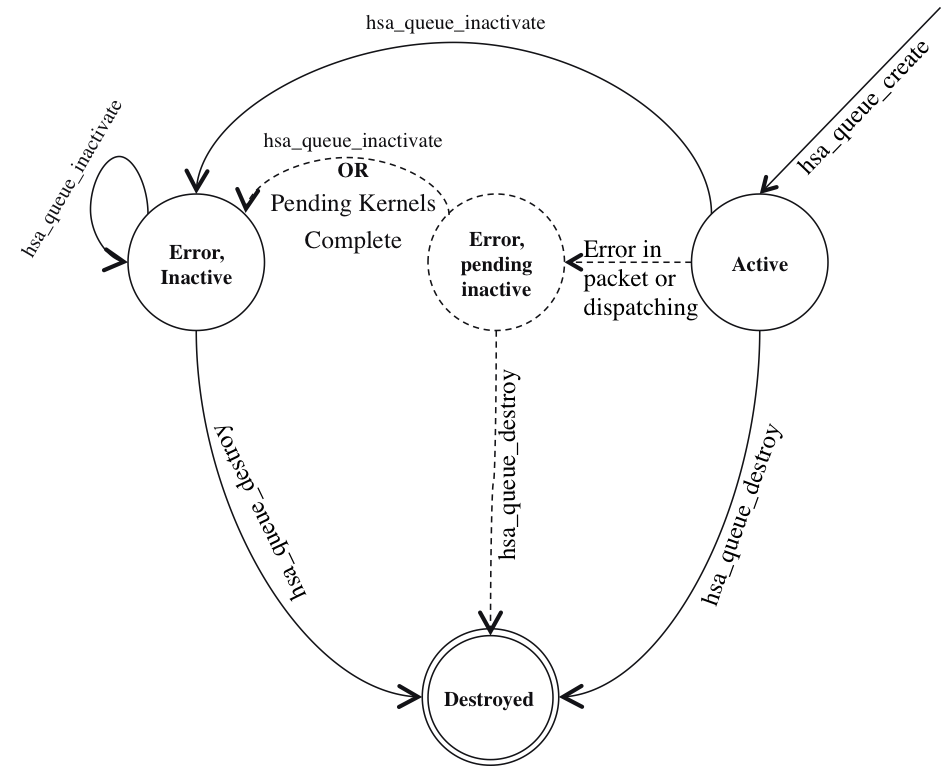
\includegraphics[width=0.5\textwidth] {fig/queuestate}
  \centering
  \caption{Once the queue is created and is active, any error in
          packet processing takes the queue into pending inactive
          state where the queue is performing tasks to get to
          inactive state. Failure during the attempt to inactivate
          results in queue reaching an error state. A queue that is
          in active, error or inactive state may be destroyed by
          using the \reffun{hsa\_queue\_destroy} API provided by
  the HSA runtime.}
  \label{fig:queuestate}
\end{SCfigure}

A state diagram showing the various states and transitions is shown
in Figure~\ref{fig:queuestate}.

The queue will report packet processing or parsing error, system
error, dependency resolution error, and signalling error (signal
destroyed by the time it needed to be signalled by packet processor).

The queue error reporting infrastructure supports and reports a
single error per queue and attempts to inactivate the queue on the
first error it encounters.

\hypertarget{coreapi_multithreading}{}\subsection{Multi-\/\-Threaded
Queue Access}\label{coreapi_multithreading}
HSA Core API does not provide explicit API for synchronized
access to the queues -- the architected queue data structure and
read/write index update API are
sufficient to allow users to implement thread-safe packet insertion
into the queue. Users can use several techniques to support
multiple concurrent writers writing AQL packets to the queue.  The
following example code illustrates one such technique -- several
other techniques that allow concurrent writes to the queue can be
utilized in a similar way.

The sample code below demonstrates a simple reader and writer logic
to do a multi-threaded queue access using the queue structure above.

\lstinputlisting{example/queue.c}


\hypertarget{coreapi_AQL}{}\section{Core Runtime Support for
AQL}\label{AQL}
AQL is a command-interface for describing a dispatch or a dependency
in a standard format for the queue packet processor.
To match with and support the AQL packet definitions in the HSA SAR,
HSA core base runtime includes structures for different types of AQL
packets.  SAR defines four different kinds of AQL packets: invalid,
component dispatch, agent dispatch and barrier.  There is a common
packet header across these three packet types and is defined by the
following structure:

\makeatletter{}

\noindent\begin{tcolorbox}[nobeforeafter,arc=0mm,colframe=white,colback=lightgray,left=0mm]
enum \hsadef{group__aql__header_1gacc655159812af0a411cc5f70b3f54881}{hsa\_aql\_packet\_type\_t}
\end{tcolorbox}
Packet type.

\noindent\textbf{Values}\\[-5mm]
\begin{longtable}{@{}>{\hangindent=2em}p{\linewidth}}
INVALID =0\\[2mm]
DISPATCH =1\\[2mm]
BARRIER =2
\end{longtable}

\noindent\begin{tcolorbox}[breakable,nobeforeafter,arc=0mm,colframe=white,colback=lightgray,left=0mm]
struct \hsadef{group__aql__header_1ga92558e047d003985bae2558febd3dd40}{hsa\_aql\_packet\_header\_t}
\vspace{-3.5mm}\begin{longtable}{@{}p{\textwidth}}
\hspace{1.7em}uint16\_t \hsaarg{format} : 8\\
\hspace{1.7em}uint16\_t \hsaarg{barrier} : 1\\
\hspace{1.7em}uint16\_t \hsaarg{acquire\_fence\_scope} : 2\\
\hspace{1.7em}uint16\_t \hsaarg{release\_fence\_scope} : 2\\
\hspace{1.7em}uint16\_t \hsaarg{reserved} : 3
\end{longtable}

\end{tcolorbox}
AQL packet header.

\noindent\textbf{Data Fields}\\[-5mm]
\begin{longtable}{@{}>{\hangindent=2em}p{\textwidth}}
\hsaarg{format}\\\hspace{2em}8 bits for describing the packet type, 0 for INVALID, 1 for COMPONENT DISPATCH, 2 for BARRIER and 4 for AGENT DISPATCH. All other values are reserved.\\[2mm]
\hsaarg{barrier}\\\hspace{2em}If set then processing of packet will only begin when all preceding packets are complete.\\[2mm]
\hsaarg{acquire\_fence\_scope}\\\hspace{2em}Determines the scope and type of the memory fence operation applied before the packet enters the active phase. Each of the values defines a particular action by HSA agents and components. The possible values are 0 (no fence is applied), 1 (The acquire fence makes memory operations made by this HSA agent prior to launch of this packet visible to this packet operation), 2 (The acquire fence makes memory operations made by HSA agents prior to launch of this packet, visible to this packet operation), and 3 (reserved).\\[2mm]
\hsaarg{release\_fence\_scope}\\\hspace{2em}Determines the scope and type of the memory fence operation applied after kernel completion but before the packet is completed. The possible values are 0 (no fence is applied), 1 (the release fence is applied to the HSA Agent only), 2 (The release fence is applied globally to the HSA System), and 3 (reserved).\\[2mm]
\hsaarg{reserved}\\\hspace{2em}must be 0
\end{longtable}

 

The \texttt{format} field in the header is used to specify
the packet type. Beyond the four packet types defined, all the
other packet types are reserved for implementation use. In addition
to this, the last 15 bits in the packet header are also reserved for
future or implementation specific use. The format field indicates
the type of the packet. Of the three packet types, the
dispatch and the barrier packet have individual packet-state
diagrams that are discussed along with their description.


\hypertarget{dispatch_packet}{}\subsection{Dispatch AQL
Packet}\label{dispatch_packet}

Dispatch packet type is used for dispatching a kernel on to a HSA
component. The dispatch AQL packet can have five different states:
\emph{on queue}, \emph{processing}, \emph{error}, \emph{active} or
\emph{complete}. Figure~\ref{fig:packetstate} shows the different
states of a packet and transitions leading to those states.

\begin{figure}
  \centering
  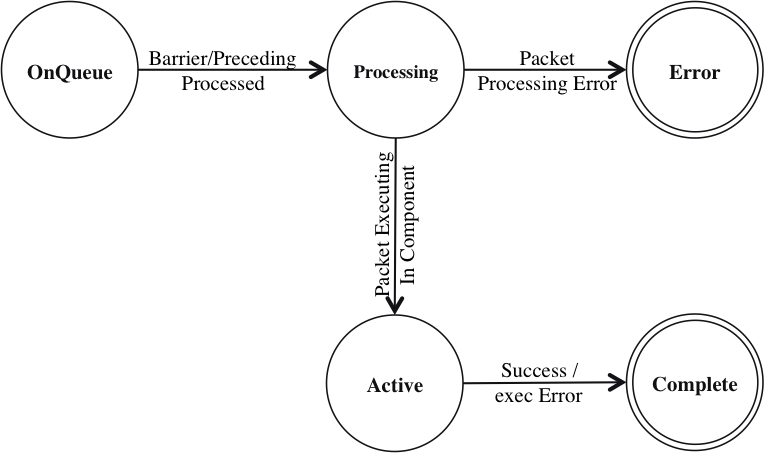
\includegraphics[width=0.5\textwidth] {fig/packetstate}
  \centering
  \caption{Dispatch Packet State Diagram}
  \label{fig:packetstate}
\end{figure}

\begin{description}
\item[On queue state] A packet is considered to be in the on queue
state once the format of the packet is changed from invalid (a value
of 0) to a value of 1, 2 or 3. Any other value for format puts the
packet and the queue in error state.

\item[Processing state] If this dispatch packet has the barrier bit
set, then the processing of this packet occurs only after all prior
kernels have completed execution.  Otherwise, once the packets prior
to this packet are processed, the packet processor begins to process
this packet and the packet enters the processing state.  From the
launch state, two states are possible: error or active.

\item[Error state] the packet processor encountered an error
processing this packet. This results in a queue error (see
Figure~\ref{fig:queuestate}) and the packet enters the error state
(the completion object is signalled with error by the packet
processor). The following errors are indicated via an error signalled
to the completion object:
processing parsing error, dependency resolution error, system error
and premature termination due to queue inactivation.
When the user invokes the
\reffun{hsa\_queue\_inactivate} API or the
\reffun{hsa\_queue\_destroy} API while the packet is in this state, the
completion object will be signalled with an error.

\item[Active state] If the packet processing is successful and the
kernel the packet represents is either executing or queued for
execution, the packet enters the active state. From active state,
either successful or failed execution both take the packet into the
completed state.  Alternatively, a user action (see
~\ref{queue_inactivate}) can also take the packet out of
active state into complete state.  When the user invokes the
\reffun{hsa\_queue\_inactivate} API or the
\reffun{hsa\_queue\_destroy} API while the packet is in this state, the
completion object will be signalled with an error.

\item[complete state] A packet enters a complete state after its
completion signal is signalled (either with success or error).
\end{description}

A dispatch packet is considered processed once the packet processor
processes it and makes the queue slot occupied by this packet
available. A processed dispatch packet may endure a period of time
where it is awaiting its dispatch on to the HSA component. Even such
packets awaiting execution are still considered as processed.

The structure for the dispatch AQL packet is shown below:
\makeatletter{}

\noindent\begin{tcolorbox}[breakable,nobeforeafter,arc=0mm,colframe=white,colback=lightgray,left=0mm]
struct \hsadef{group__dispatch__packet_1gab3d5ded5ac53f70931768468c0c0cfd6}{hsa\_aql\_dispatch\_packet\_t}
\vspace{-3.5mm}\begin{longtable}{@{}p{\textwidth}}
\hspace{1.7em}\hsatyp{group__aql__header_1ga92558e047d003985bae2558febd3dd40}{hsa\_aql\_packet\_header\_t} \hsaarg{header}\\
\hspace{1.7em}uint16\_t \hsaarg{workgroup\_size\_x}\\
\hspace{1.7em}uint16\_t \hsaarg{workgroup\_size\_y}\\
\hspace{1.7em}uint16\_t \hsaarg{workgroup\_size\_z}\\
\hspace{1.7em}uint16\_t \hsaarg{reserved2}\\
\hspace{1.7em}uint32\_t \hsaarg{grid\_size\_x}\\
\hspace{1.7em}uint32\_t \hsaarg{grid\_size\_y}\\
\hspace{1.7em}uint32\_t \hsaarg{grid\_size\_z}\\
\hspace{1.7em}uint32\_t \hsaarg{private\_segment\_size\_bytes}\\
\hspace{1.7em}uint32\_t \hsaarg{group\_segment\_size\_bytes}\\
\hspace{1.7em}uint64\_t \hsaarg{kernel\_object\_address}\\
\hspace{1.7em}uint64\_t \hsaarg{kernarg\_address}\\
\hspace{1.7em}uint64\_t \hsaarg{reserved3}\\
\hspace{1.7em}\hsatyp{group__signal__value_1ga6592c136d70853d855bc11d9efdbf534}{hsa\_signal\_handle\_t} \hsaarg{completion\_signal}
\end{longtable}

\end{tcolorbox}
AQL dispatch packet.

\noindent\textbf{Data Fields}\\[-5mm]
\begin{longtable}{@{}>{\hangindent=2em}p{\textwidth}}
\hsaarg{header}\\\hspace{2em}Packet header structure\\[2mm]
\hsaarg{workgroup\_size\_x}\\\hspace{2em}X dimension of work-group (measured in work-items).\\[2mm]
\hsaarg{workgroup\_size\_y}\\\hspace{2em}Y dimension of work-group (measured in work-items).\\[2mm]
\hsaarg{workgroup\_size\_z}\\\hspace{2em}Z dimension of work-group (measured in work-items).\\[2mm]
\hsaarg{reserved2}\\\hspace{2em}Reserved\\[2mm]
\hsaarg{grid\_size\_x}\\\hspace{2em}X dimension of grid (measured in work-items).\\[2mm]
\hsaarg{grid\_size\_y}\\\hspace{2em}Y dimension of grid (measured in work-items).\\[2mm]
\hsaarg{grid\_size\_z}\\\hspace{2em}Z dimension of grid (measured in work-items).\\[2mm]
\hsaarg{private\_segment\_size\_bytes}\\\hspace{2em}Size (in bytes) of private memory allocation request per work-item.\\[2mm]
\hsaarg{group\_segment\_size\_bytes}\\\hspace{2em}Size (in bytes) of group memory allocation request per work-group.\\[2mm]
\hsaarg{kernel\_object\_address}\\\hspace{2em}Address of an object in memory that includes an implementation-defined executable ISA image for the kernel.\\[2mm]
\hsaarg{kernarg\_address}\\\hspace{2em}Address of memory containing kernel arguments.\\[2mm]
\hsaarg{reserved3}\\\hspace{2em}Reserved.\\[2mm]
\hsaarg{completion\_signal}\\\hspace{2em}HSA signaling object used to indicate completion of the job.
\end{longtable}

 

\hypertarget{segment_sizes}{}\subsubsection{Segment
Sizes}\label{segment_sizes}
If the kernel being dispatched uses private and group segments, the
user is required to specify the sizes of these segments in the AQL
dispatch packet. Manually calculating this information is not
feasible and requires visual inspection of the user program, which itself
may have been generated by a higher-level compiler. Hence the user
must rely on the \texttt{finalizer} to get the corresponding segment
sizes. Further details about determining segment sizes are described in
Section~\ref{finalizerchapter}.

Of the other HSA segments, the kernarg segment is also a part of the
AQL packet, but as a pointer. This is because the kernarg segment
carries the arguments required to execute the kernel being dispatched
and must be setup by the user (the layout of this segment is
language/finalization specific and associated with the code object
generated by finalization) prior to writing the AQL packet to the
queue (unlike the group and private segments, whose lifespan spans
only the active state of the AQL dispatch packet).  Please refer to
the HSAIL service layer for an example on how to setup the kernarg
segment for the HSAIL language, which is based on the 32/64 bit modes
the kernel is compiled in.

\hypertarget{agent_packet}{}\subsection{Agent Dispatch AQL
Packet}\label{agent_packet}
Agent Dispatch AQL packets can be used to do dispatches on the agent
queue. The HSA Queue API allows for creation of either agent queues
or component queues in the core API (vendor-specific extensions may
support queues that allow both agent and component dispatches, but
it is not a core feature). The HSA core runtime structure for agent
dispatches is defined as follows:

\makeatletter{}

\noindent\begin{tcolorbox}[breakable,nobeforeafter,arc=0mm,colframe=white,colback=lightgray,left=0mm]
struct \hsadef{group__agent__packet_1ga07dc7a6c787b5bee6e3f0b8b79586109}{hsa\_aql\_agent\_dispatch\_packet\_t}
\vspace{-3.5mm}\begin{longtable}{@{}p{\textwidth}}
\hspace{1.7em}\hsatyp{group__aql__header_1ga92558e047d003985bae2558febd3dd40}{hsa\_aql\_packet\_header\_t} \hsaarg{header}\\
\hspace{1.7em}uint16\_t \hsaarg{type}\\
\hspace{1.7em}uint32\_t \hsaarg{reserved2}\\
\hspace{1.7em}uint64\_t \hsaarg{returnLocation}\\
\hspace{1.7em}uint64\_t \hsaarg{arg0}\\
\hspace{1.7em}uint64\_t \hsaarg{arg1}\\
\hspace{1.7em}uint64\_t \hsaarg{arg2}\\
\hspace{1.7em}uint64\_t \hsaarg{arg3}\\
\hspace{1.7em}uint64\_t \hsaarg{reserved3}\\
\hspace{1.7em}uint64\_t \hsaarg{completionSignal}
\end{longtable}

\end{tcolorbox}
Agent dispatch packet.

\noindent\textbf{Data Fields}\\[-5mm]
\begin{longtable}{@{}>{\hangindent=2em}p{\textwidth}}
\hsaarg{header}\\\hspace{2em}Packet header structure\\[2mm]
\hsaarg{type}\\\hspace{2em}The function to be performed by the destination HSA Agent. The type value is split into the following ranges: 0x0000:0x3FFF – Vendor specific 0x4000:0x7FFF – HSA runtime 0x8000:0xFFFF – User registered function\\[2mm]
\hsaarg{reserved2}\\\hspace{2em}Reserved. Must be 0.\\[2mm]
\hsaarg{returnLocation}\\\hspace{2em}Pointer to location to store the function return value(s) in.\\[2mm]
\hsaarg{arg0}\\\hspace{2em}64-bit direct or indirect arguments.\\[2mm]
\hsaarg{arg1}\\\hspace{2em}64-bit direct or indirect arguments.\\[2mm]
\hsaarg{arg2}\\\hspace{2em}64-bit direct or indirect arguments.\\[2mm]
\hsaarg{arg3}\\\hspace{2em}64-bit direct or indirect arguments.\\[2mm]
\hsaarg{reserved3}\\\hspace{2em}Reserved. Must be 0.\\[2mm]
\hsaarg{completionSignal}\\\hspace{2em}Address of HSA signaling object used to indicate completion of the job.
\end{longtable}

 

\hypertarget{barrier_packet}{}\subsection{Barrier AQL
packet}\label{barrier_packet}
The barrier packet allows the user to specify up to 5 dependencies
as \reftyp{hsa\_signal} objects and requires the packet processor to
resolve them before proceeding. The barrier packet is a blocking
packet, in that the processing of the barrier packet
\emph{completes} the packet and its completion object is signalled.
This is unlike a dispatch packet whose completion may occur at some
future time after the packet has finished processing. The HSA core
runtime structure for the AQL barrier packet is shown below:

\makeatletter{}

\noindent\begin{tcolorbox}[breakable,nobeforeafter,arc=0mm,colframe=white,colback=lightgray,left=0mm]
struct \hsadef{group__barrier__packet_1ga8e5ebbeffbf5af1ece8db9ef27c14715}{hsa\_aql\_barrier\_packet\_t}
\vspace{-3.5mm}\begin{longtable}{@{}p{\textwidth}}
\hspace{1.7em}\hsatyp{group__aql__header_1ga92558e047d003985bae2558febd3dd40}{hsa\_aql\_packet\_header\_t} \hsaarg{header}\\
\hspace{1.7em}uint32\_t \hsaarg{reserved2}\\
\hspace{1.7em}uint64\_t \hsaarg{dep\_signal0}\\
\hspace{1.7em}uint64\_t \hsaarg{dep\_signal1}\\
\hspace{1.7em}uint64\_t \hsaarg{dep\_signal2}\\
\hspace{1.7em}uint64\_t \hsaarg{dep\_signal3}\\
\hspace{1.7em}uint64\_t \hsaarg{dep\_signal4}\\
\hspace{1.7em}uint64\_t \hsaarg{reserved3}\\
\hspace{1.7em}uint64\_t \hsaarg{completion\_signal}
\end{longtable}

\end{tcolorbox}
Barrier packet.

\noindent\textbf{Data Fields}\\[-5mm]
\begin{longtable}{@{}>{\hangindent=2em}p{\textwidth}}
\hsaarg{header}\\\hspace{2em}Packet header structure.\\[2mm]
\hsaarg{reserved2}\\\hspace{2em}Reserved.\\[2mm]
\hsaarg{dep\_signal0}\\\hspace{2em}The first dependency signal, a negative value means dependency not met and the completion signal for this packet will be set to.\\[2mm]
\hsaarg{dep\_signal1}\\\hspace{2em}The first dependency signal, a negative value means dependency not met and the completion signal for this packet will be set to\\[2mm]
\hsaarg{dep\_signal2}\\\hspace{2em}The first dependency signal, a negative value means dependency not met and the completion signal for this packet will be set to.\\[2mm]
\hsaarg{dep\_signal3}\\\hspace{2em}The first dependency signal, a negative value means dependency not met and the completion signal for this packet will be set to.\\[2mm]
\hsaarg{dep\_signal4}\\\hspace{2em}The first dependency signal, a negative value means dependency not met and the completion signal for this packet will be set to.\\[2mm]
\hsaarg{reserved3}\\\hspace{2em}Reserved.\\[2mm]
\hsaarg{completion\_signal}\\\hspace{2em}HSA signaling object used to indicate completion of the dependency resolution, success of failure
\end{longtable}

 

If any of the dependent signals have been signalled with a negative
value, the barrier packet is complete, and will indicate failure in
its completion signal. The \texttt{completion signal} will be
signalled with the error value as discussed in
Section~\ref{signal_error}. If the queue is not already in an error
state (e.g. the job generating the error was processed in a different
queue) then the HSA Packet Processor should consider the error code on
the dependent signal to indicate an error in the queue itself and
subsequently signal the \reffld{error\_signal} in the queue. When all
of the dependent signals have been signalled with the value 0, the
\reffld{completion\_signal} will be signalled with the value 0 to
indicate a successful completion.

The barrier packet also has a barrier bit that indicates that this
packet may only be processed when all previous packets have been
marked as completed.

Alike the dispatch packet, the barrier packet can also be in one of
the following states: \emph{on queue}, \emph{processing},
\emph{completed, error} or \emph{completed, success}. The state
diagram in Figure~\ref{fig:barrierpacketstate} shows the transitions
between these states.

\begin{figure}
  \centering
  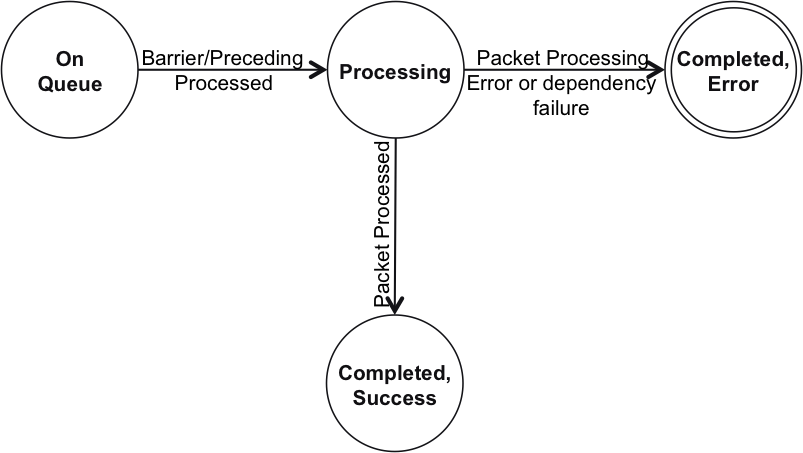
\includegraphics[width=0.5\textwidth] {fig/barrierpacketstate}
  \centering
  \caption{Barrier Packet State Diagram}
  \label{fig:barrierpacketstate}
\end{figure}

\begin{description}
\item[On queue state] A packet is considered to be in the on queue
state once the format of the packet is changed from invalid (a value
of 0) to a value of 1 or 2 or 3. Any other value for format puts the
packet and the queue in error state.
\item[Processing state] If this barrier packet has the barrier bit set,
then the processing of this packet occurs only after all prior
dispatch packets have completed execution.  Otherwise, once the
packets prior to this packet are processed, the packet processor
begins to process this packet and the packet enters the processing
state.  From the launch state, two states are possible: completion,
error or completion, success.
\item[completed-error] The barrier packet reaches this state from
the processing state if (a) one of the dependency signals had an
error, and (b) if the packet was malformed (e.g. bad signal object
or invalid usage of reserved bits). A barrier packet can also reach
this state when the user invokes the \reffun{hsa\_queue\_inactivate}
API or the \reffun{hsa\_queue\_destroy} API while the packet is in
processing state (the completion object will be appropriately
signalled with an error).
\item[completed-success] The barrier packet had all its dependencies
met, its completion object has been signalled with a value of 0.
\end{description}
\hypertarget{aql_example}{}\subsection{Packet Setup
Example}\label{aql_example}
TODO
\hypertarget{coreapi_memory_registration}{}\section{Memory Registration and Deregistration}\label{coreapi_memory_registration}

\hypertarget{coreapi_registration_overview}{}\subsection{Overview}\label{coreapi_registration_overview}
One of the key features of HSA is its ability to share global
pointers between the host application and code executing on the
component. This ability means that an application can directly pass a
pointer to memory allocated on the host to a kernel function
dispatched to a component without an intermediate copy, as illustrated
by the example shown in \hyperlink{coreapi}{Core API
Documentation}.

When a buffer will be accessed by a kernel running on a HSA
device, programmers are encouraged to register the corresponding
address range beforehand by using the appropriate HSA core
API invocation. While kernels running on HSA devices can
access any valid system memory pointer allocated by means of
standard libraries (for example, malloc in the C language) without
resorting to registration, there might be a performance benefit from
registering the buffer with the HSA core component. When an
HSA program no longer needs to access a registered buffer in a
device, the user should deregister that virtual address range by
using the appropriate HSA core API invocation.

\makeatletter{}

\noindent\begin{tcolorbox}[breakable,nobeforeafter,colframe=white,colback=lightgray,left=0mm]
\hsatyp{group__status_1gad755322e7ff95456520e8abdbe90d225}{hsa\_status\_t} \hsadef{group__register_1ga13131274af7b6c583b689eaaca3e21f0}{hsa\_memory\_register}(
\vspace{-3.5mm}\begin{longtable}{@{}p{\textwidth}}
\hspace{1.7em}void * \hsaarg{address},\\
\hspace{1.7em}size\_t \hsaarg{size})\end{longtable}

\end{tcolorbox}
Register memory.

\noindent\textbf{Parameters}\\[-6mm]
\noindent\begin{longtable}{@{}>{\hangindent=2em}p{\textwidth}}
\hsaarg{address}\\\hspace{2em}(in) A pointer to the base of the memory region to be registered. If a null pointer is passed, no operation is performed.\\[2mm]
\hsaarg{size}\\\hspace{2em}(in) Requested registration size in bytes. If a size of zero is passed, no operation is performed.
\end{longtable}
\vspace{-5mm}\noindent\textbf{Return Values}\\[-6mm]
\noindent\begin{longtable}{@{}>{\hangindent=2em}p{\linewidth}}
\hsatyp{group__status_1ggad755322e7ff95456520e8abdbe90d225ae382ea0c9c05cce5a60d0317375159cc}{HSA\_STATUS\_SUCCESS}\\\hspace{2em}If successful\\[2mm]
\hsatyp{group__status_1ggad755322e7ff95456520e8abdbe90d225a1a77fcf36d0d140874c4361ab093eff7}{HSA\_STATUS\_ERROR\_OUT\_OF\_RESOURCES}\\\hspace{2em}If there is a failure in allocating the necessary resources.
\end{longtable}
\vspace{-4mm}\noindent\textbf{Description}\\[1mm]
Registering a system memory region for use with all the available devices This is an optional interface that is solely provided as a performance optimization hint to the underlying implementation so it may prepare for the future use of the memory by the devices. The interface is only beneficial for system memory that will be directly accessed by a device.\\[2mm]
Overlapping registrations are allowed. This is neither detrimental nor beneficial. 


\noindent\begin{tcolorbox}[breakable,nobeforeafter,colframe=white,colback=lightgray,left=0mm]
\hsatyp{group__status_1gad755322e7ff95456520e8abdbe90d225}{hsa\_status\_t} \hsadef{group__register_1gab577eaa466b4315f9545e59fdd4b7ec9}{hsa\_memory\_deregister}(
\vspace{-3.5mm}\begin{longtable}{@{}p{\textwidth}}
\hspace{1.7em}void * \hsaarg{address})\end{longtable}

\end{tcolorbox}
Deregister memory.

\noindent\textbf{Parameters}\\[-6mm]
\noindent\begin{longtable}{@{}>{\hangindent=2em}p{\textwidth}}
\hsaarg{address}\\\hspace{2em}(in) A pointer to the base of the memory region to be deregistered. If a NULL pointer is passed, no operation is performed.
\end{longtable}
\vspace{-5mm}\noindent\textbf{Return Values}\\[-6mm]
\noindent\begin{longtable}{@{}>{\hangindent=2em}p{\linewidth}}
\hsatyp{group__status_1ggad755322e7ff95456520e8abdbe90d225ae382ea0c9c05cce5a60d0317375159cc}{HSA\_STATUS\_SUCCESS}\\\hspace{2em}If successful\\[2mm]
\hsatyp{group__status_1ggad755322e7ff95456520e8abdbe90d225a19fef906a58c2b743e9b375a016582a7}{HSA\_STATUS\_INFO\_NOT\_REGISTERED}\\\hspace{2em}If the pointer has not been registered before.
\end{longtable}
\vspace{-4mm}\noindent\textbf{Description}\\[1mm]
Used for deregistering a memory region previously registered.\\[2mm]
Deregistration must be performed using an address that was previously registered. In the event that deregistration is performed on an address that has been used in multiple registrations, the smallest of the registrations is deregistered. 
 

\hypertarget{coreapi_registration_usage}{}\subsection{Usage}\label{coreapi_registration_usage}

A buffer is registered by indicating its starting address and a
size. The size does not need to match that of the original
allocation. For example:

\begin{lstlisting}
void* ptr = malloc(16);
status = hsa_memory_register(ptr, 8);
if(status == HSA_STATUS_ERROR_INVALID_ARGUMENT)
  handle_error(status);
\end{lstlisting}

 is a valid program. On the other hand:

\begin{lstlisting}
void* ptr = malloc(16);
status = hsa_memory_register(ptr, 20);
if(status == HSA_STATUS_ERROR_INVALID_ARGUMENT)
  handle_error(status);
\end{lstlisting}

is not a valid program, because we are registering a range that
spans several allocations, or might not be entirely allocated.

Registrations can overlap previously registered intervals. A special
case of overlapped registrations is multiple registration. If the
same interval is registered several times with different sizes, the
HSA core component will select the maximum as the size of all
the registrations. Therefore, the following program:

\begin{lstlisting}
status = hsa_memory_register(ptr, 8);
if(status == HSA_STATUS_ERROR_INVALID_ARGUMENT)
  handle_error(status);
status = hsa_memory_register(ptr, 16);
if(status == HSA_STATUS_ERROR_INVALID_ARGUMENT)
  handle_error(status);
\end{lstlisting}

behaves identically to this program:

\begin{lstlisting}
hsa_memory_register(ptr, 16);
if(status == HSA_STATUS_ERROR_INVALID_ARGUMENT)
  handle_error(status);
hsa_memory_register(ptr, 16);
if(status == HSA_STATUS_ERROR_INVALID_ARGUMENT)
  handle_error(status);
\end{lstlisting}

While the described behavior might seem counterintuitive, consider
the following scenario: A pointer is registered twice with
different sizes s1 and s2. When the pointer is deregistered, which
interval should be deregistered: (p, s1) or (p, s2)? If all the
registrations of the same pointer are considered identical by the
core runtime, that problem is eliminated.

Deregistering a pointer that has not been previously registered
results in an \emph{info} status indicating the same.

The following code snippet revisits the introductory example. The
code is almost identical to the original, except that we register
the buffers that will be accessed from the device after allocating
them, and we deregister all that memory before releasing it. In some
platforms, we expect this version to perform better than the
original one.


\hypertarget{coreapi_device_memory}{}\section{Memory Allocation
and Copy}\label{coreapi_device_memory}

While a HSA component is capable of accessing pageable system memory
by definition, for scenarios where wants memory allocated that has
already been registered (combine the allocation with memory
registration described in
Section~\ref{coreapi_registration_overview}), the HSA runtime
provides an interface, \reffun{hsa\_memory\_allocate} to allocate
memory that is internally registered by the runtime:

\makeatletter{}

\noindent\begin{tcolorbox}[breakable,nobeforeafter,colframe=white,colback=lightgray,left=0mm]
\hsatyp{group__status_1gad755322e7ff95456520e8abdbe90d225}{hsa\_status\_t} \hsadef{group__memory__allocate_1gae86946629841221ce6ec2819fbad6e80}{hsa\_memory\_allocate}(
\vspace{-3.5mm}\begin{longtable}{@{}p{\textwidth}}
\hspace{1.7em}size\_t \hsaarg{size\_bytes},\\
\hspace{1.7em}void ** \hsaarg{address})\end{longtable}

\end{tcolorbox}
Allocate system memory.

\noindent\textbf{Parameters}\\[-6mm]
\noindent\begin{longtable}{@{}>{\hangindent=2em}p{\textwidth}}
\hsaarg{size\_bytes}\\\hspace{2em}(in) Allocation size.\\[2mm]
\hsaarg{address}\\\hspace{2em}(in) Address pointer allocated by the user. Dereferenced and assigned to the pointer to the memory allocated for this request.
\end{longtable}
\vspace{-5mm}\noindent\textbf{Return Values}\\[-6mm]
\noindent\begin{longtable}{@{}>{\hangindent=2em}p{\linewidth}}
\hsatyp{group__status_1ggad755322e7ff95456520e8abdbe90d225ae382ea0c9c05cce5a60d0317375159cc}{HSA\_STATUS\_SUCCESS}\\\hspace{2em}If successful\\[2mm]
\hsatyp{group__status_1ggad755322e7ff95456520e8abdbe90d225a1a77fcf36d0d140874c4361ab093eff7}{HSA\_STATUS\_ERROR\_OUT\_OF\_RESOURCES}\\\hspace{2em}If there is a failure in allocation. This error may also occur when the core runtime library needs to spawn threads or create internal OS-specific events.\\[2mm]
\hsatyp{group__status_1ggad755322e7ff95456520e8abdbe90d225ac7d3651f75107d2a6a8ba3b25683c030}{HSA\_STATUS\_ERROR\_INVALID\_ARGUMENT}\\\hspace{2em}If the passed address is NULL.
\end{longtable}
\vspace{-4mm}\noindent\textbf{Description}\\[1mm]
The returned buffer is already registerd. Allocation of size 0 is allowed and returns a NULL pointer. 
 

\hypertarget{coreapi_kernarg}{}\subsection{Kernarg
Memory}\label{kernargmem}

The kernarg memory that AQL packet points to (see Section~\ref{AQL})
holds information about any arguments required to execute AQL dispatch
on a HSA component. While any system memory may be used for kernarg
memory, implementation/platform specific optimizations are possible if
HSA core runtime provided API are utilized for allocating and copying
to the allocated kernarg memory. To facilitate such optimizations, HSA
core runtime defines the following API:

\makeatletter{}

\noindent\begin{tcolorbox}[breakable,nobeforeafter,colframe=white,colback=lightgray,left=0mm]
\hsatyp{group__status_1gad755322e7ff95456520e8abdbe90d225}{hsa\_status\_t} \hsadef{group__kernargmem_1ga9bcec6a182d021007b4c5c2b6b0467fc}{hsa\_memory\_allocate\_kernarg}(
\vspace{-3.5mm}\begin{longtable}{@{}p{\textwidth}}
\hspace{1.7em}const \hsatyp{group__component_1gab8db3fb886332a24acac08ec361e1d86}{hsa\_agent\_t} * \hsaarg{component},\\
\hspace{1.7em}size\_t \hsaarg{size},\\
\hspace{1.7em}void ** \hsaarg{address})\end{longtable}

\end{tcolorbox}
Allocate kernarg memory.

\noindent\textbf{Parameters}\\[-6mm]
\noindent\begin{longtable}{@{}>{\hangindent=2em}p{\textwidth}}
\hsaarg{component}\\\hspace{2em}(in) A valid pointer to the component for which the specified amount of kernarg memory is to be allocated.\\[2mm]
\hsaarg{size}\\\hspace{2em}(in) Requested allocation size in bytes. If size is 0, NULL is returned.\\[2mm]
\hsaarg{address}\\\hspace{2em}(out) A valid pointer to the location of where to return the pointer to the base of the allocated region of memory.
\end{longtable}
\vspace{-5mm}\noindent\textbf{Return Values}\\[-6mm]
\noindent\begin{longtable}{@{}>{\hangindent=2em}p{\linewidth}}
\hsatyp{group__status_1ggad755322e7ff95456520e8abdbe90d225ae382ea0c9c05cce5a60d0317375159cc}{HSA\_STATUS\_SUCCESS}\\\hspace{2em}If successful.\\[2mm]
\hsatyp{group__status_1ggad755322e7ff95456520e8abdbe90d225ac7d3651f75107d2a6a8ba3b25683c030}{HSA\_STATUS\_ERROR\_INVALID\_ARGUMENT}\\\hspace{2em}if the passed address is NULL.
\end{longtable}
 


\noindent\begin{tcolorbox}[breakable,nobeforeafter,colframe=white,colback=lightgray,left=0mm]
\hsatyp{group__status_1gad755322e7ff95456520e8abdbe90d225}{hsa\_status\_t} \hsadef{group__kernargmem_1gaa47857aa28d4a7e1824a8ca68e691e31}{hsa\_memory\_copy\_kernarg\_to\_system}(
\vspace{-3.5mm}\begin{longtable}{@{}p{\textwidth}}
\hspace{1.7em}void * \hsaarg{dst},\\
\hspace{1.7em}const void * \hsaarg{src},\\
\hspace{1.7em}size\_t \hsaarg{size})\end{longtable}

\end{tcolorbox}
Copy between the system and kernarg segments.

\noindent\textbf{Parameters}\\[-6mm]
\noindent\begin{longtable}{@{}>{\hangindent=2em}p{\textwidth}}
\hsaarg{dst}\\\hspace{2em}(out) A valid pointer to the destination array where the content is to be copied.\\[2mm]
\hsaarg{src}\\\hspace{2em}(in) A valid pointer to the source of data to be copied.\\[2mm]
\hsaarg{size}\\\hspace{2em}(in) Number of bytes to copy.
\end{longtable}
\vspace{-5mm}\noindent\textbf{Return Values}\\[-6mm]
\noindent\begin{longtable}{@{}>{\hangindent=2em}p{\linewidth}}
\hsatyp{group__status_1ggad755322e7ff95456520e8abdbe90d225ae382ea0c9c05cce5a60d0317375159cc}{HSA\_STATUS\_SUCCESS}\\\hspace{2em}If successful.\\[2mm]
\hsatyp{group__status_1ggad755322e7ff95456520e8abdbe90d225ac7d3651f75107d2a6a8ba3b25683c030}{HSA\_STATUS\_ERROR\_INVALID\_ARGUMENT}\\\hspace{2em}if the source or destination pointers are invalid.
\end{longtable}
 


\noindent\begin{tcolorbox}[breakable,nobeforeafter,colframe=white,colback=lightgray,left=0mm]
\hsatyp{group__status_1gad755322e7ff95456520e8abdbe90d225}{hsa\_status\_t} \hsadef{group__kernargmem_1gae89ae228189add9fffc3d6c41355056b}{hsa\_memory\_copy\_system\_to\_kernarg}(
\vspace{-3.5mm}\begin{longtable}{@{}p{\textwidth}}
\hspace{1.7em}void * \hsaarg{dst},\\
\hspace{1.7em}const void * \hsaarg{src},\\
\hspace{1.7em}size\_t \hsaarg{size})\end{longtable}

\end{tcolorbox}
Copy between the system and kernarg segments.

\noindent\textbf{Parameters}\\[-6mm]
\noindent\begin{longtable}{@{}>{\hangindent=2em}p{\textwidth}}
\hsaarg{dst}\\\hspace{2em}(out) A valid pointer to the destination array where the content is to be copied.\\[2mm]
\hsaarg{src}\\\hspace{2em}(in) A valid pointer to the source of data to be copied.\\[2mm]
\hsaarg{size}\\\hspace{2em}(in) Number of bytes to copy.
\end{longtable}
\vspace{-5mm}\noindent\textbf{Return Values}\\[-6mm]
\noindent\begin{longtable}{@{}>{\hangindent=2em}p{\linewidth}}
\hsatyp{group__status_1ggad755322e7ff95456520e8abdbe90d225ae382ea0c9c05cce5a60d0317375159cc}{HSA\_STATUS\_SUCCESS}\\\hspace{2em}If successful.\\[2mm]
\hsatyp{group__status_1ggad755322e7ff95456520e8abdbe90d225ac7d3651f75107d2a6a8ba3b25683c030}{HSA\_STATUS\_ERROR\_INVALID\_ARGUMENT}\\\hspace{2em}if the source or destination pointers are invalid.
\end{longtable}
 
 

\hypertarget{coreapi_device_memory}{}\subsection{Component Local
  Memory}\label{coreapi_device_memory}

Component local memory is a memory type that is dedicated specifically
for a particular HSA component. This memory could provide higher
bandwidth for component access (than system memory) with the
limitation that the host might not be able to access it directly. HSA
runtime provides a host interface to allocate/deallocate and access
component local memory.

\makeatletter{}

\noindent\begin{tcolorbox}[breakable,nobeforeafter,colframe=white,colback=lightgray,left=0mm]
\hsatyp{group__status_1gad755322e7ff95456520e8abdbe90d225}{hsa\_status\_t} \hsadef{group__memory__local_1ga40d441131fce376e8c65ae5087bc916a}{hsa\_memory\_allocate\_component\_local}(
\vspace{-3.5mm}\begin{longtable}{@{}p{\textwidth}}
\hspace{1.7em}const \hsatyp{group__component_1gab8db3fb886332a24acac08ec361e1d86}{hsa\_agent\_t} * \hsaarg{component},\\
\hspace{1.7em}size\_t \hsaarg{size},\\
\hspace{1.7em}void ** \hsaarg{address})\end{longtable}

\end{tcolorbox}
Allocate memory on HSA Device.

\noindent\textbf{Parameters}\\[-6mm]
\noindent\begin{longtable}{@{}>{\hangindent=2em}p{\textwidth}}
\hsaarg{component}\\\hspace{2em}(in) A valid pointer to the HSA device for which the specified amount of global memory is to be allocated.\\[2mm]
\hsaarg{size}\\\hspace{2em}(in) Requested allocation size in bytes. If size is 0, NULL is returned.\\[2mm]
\hsaarg{address}\\\hspace{2em}(out) A valid pointer to the location of where to return the pointer to the base of the allocated region of memory.
\end{longtable}
\vspace{-5mm}\noindent\textbf{Return Values}\\[-6mm]
\noindent\begin{longtable}{@{}>{\hangindent=2em}p{\linewidth}}
\hsatyp{group__status_1ggad755322e7ff95456520e8abdbe90d225ae382ea0c9c05cce5a60d0317375159cc}{HSA\_STATUS\_SUCCESS}\\\hspace{2em}If successful\\[2mm]
\hsatyp{group__status_1ggad755322e7ff95456520e8abdbe90d225a1a77fcf36d0d140874c4361ab093eff7}{HSA\_STATUS\_ERROR\_OUT\_OF\_RESOURCES}\\\hspace{2em}If there is a failure in allocation of an internal structure required by the core runtime library. This error may also occur when the core runtime library needs to spawn threads or create internal OS-specific events.\\[2mm]
\hsatyp{group__status_1ggad755322e7ff95456520e8abdbe90d225ac7d3651f75107d2a6a8ba3b25683c030}{HSA\_STATUS\_ERROR\_INVALID\_ARGUMENT}\\\hspace{2em}If the passed component is NULL or invalid, or if the passed pointer is NULL.
\end{longtable}
\vspace{-4mm}\noindent\textbf{Description}\\[1mm]
Allocate global device memory associated with specified device. 


\noindent\begin{tcolorbox}[breakable,nobeforeafter,colframe=white,colback=lightgray,left=0mm]
\hsatyp{group__status_1gad755322e7ff95456520e8abdbe90d225}{hsa\_status\_t} \hsadef{group__memory__local_1gab7716a76b328a81dc0657a4b38faa945}{hsa\_memory\_free\_component\_local}(
\vspace{-3.5mm}\begin{longtable}{@{}p{\textwidth}}
\hspace{1.7em}void * \hsaarg{address})\end{longtable}

\end{tcolorbox}
Deallocate memory on HSA component.

\noindent\textbf{Parameters}\\[-6mm]
\noindent\begin{longtable}{@{}>{\hangindent=2em}p{\textwidth}}
\hsaarg{address}\\\hspace{2em}(in) A pointer to the address to be deallocated. If the pointer is NULL, no operation is performed.
\end{longtable}
\vspace{-5mm}\noindent\textbf{Return Values}\\[-6mm]
\noindent\begin{longtable}{@{}>{\hangindent=2em}p{\linewidth}}
\hsatyp{group__status_1ggad755322e7ff95456520e8abdbe90d225ae382ea0c9c05cce5a60d0317375159cc}{HSA\_STATUS\_SUCCESS}\\\hspace{2em}If successful
\end{longtable}
\vspace{-4mm}\noindent\textbf{Description}\\[1mm]
Deallocate global device memory that was previously allocated with \hsatyp{group__memory__local_1ga40d441131fce376e8c65ae5087bc916a}{hsa\_memory\_allocate\_component\_local}. 


\noindent\begin{tcolorbox}[breakable,nobeforeafter,colframe=white,colback=lightgray,left=0mm]
\hsatyp{group__status_1gad755322e7ff95456520e8abdbe90d225}{hsa\_status\_t} \hsadef{group__memory__local_1ga5733ddfc7ac81df2892396e0ada66bad}{hsa\_memory\_copy\_component\_local\_to\_system}(
\vspace{-3.5mm}\begin{longtable}{@{}p{\textwidth}}
\hspace{1.7em}void * \hsaarg{dst},\\
\hspace{1.7em}const void * \hsaarg{src},\\
\hspace{1.7em}size\_t \hsaarg{size},\\
\hspace{1.7em}\hsatyp{group__signal__value_1ga6592c136d70853d855bc11d9efdbf534}{hsa\_signal\_handle\_t} \hsaarg{signal})\end{longtable}

\end{tcolorbox}
Copy between the system and local heaps.

\noindent\textbf{Parameters}\\[-6mm]
\noindent\begin{longtable}{@{}>{\hangindent=2em}p{\textwidth}}
\hsaarg{dst}\\\hspace{2em}(out) A valid pointer to the destination array where the content is to be copied.\\[2mm]
\hsaarg{src}\\\hspace{2em}(in) A valid pointer to the source of data to be copied.\\[2mm]
\hsaarg{size}\\\hspace{2em}(in) Number of bytes to copy.\\[2mm]
\hsaarg{signal}\\\hspace{2em}(in) The signal that will be incremented by the runtime when the copy is complete.
\end{longtable}
\vspace{-5mm}\noindent\textbf{Return Values}\\[-6mm]
\noindent\begin{longtable}{@{}>{\hangindent=2em}p{\linewidth}}
\hsatyp{group__status_1ggad755322e7ff95456520e8abdbe90d225ae382ea0c9c05cce5a60d0317375159cc}{HSA\_STATUS\_SUCCESS}\\\hspace{2em}If successful\\[2mm]
\hsatyp{group__status_1ggad755322e7ff95456520e8abdbe90d225a1a77fcf36d0d140874c4361ab093eff7}{HSA\_STATUS\_ERROR\_OUT\_OF\_RESOURCES}\\\hspace{2em}If there is a failure in allocation of an internal structure required by the core runtime library. This error may also occur when the core runtime library needs to spawn threads or create internal OS-specific events.\\[2mm]
\hsatyp{group__status_1ggad755322e7ff95456520e8abdbe90d225ac7d3651f75107d2a6a8ba3b25683c030}{HSA\_STATUS\_ERROR\_INVALID\_ARGUMENT}\\\hspace{2em}If any argument is invalid.
\end{longtable}
 
 

\hypertarget{coreapi_device_memory_usage}{}\subsection{Usage}\label{coreapi_device_memory_usage}

Component memory is allocated by indicating the size and the HSA
device it corresponds to. For example, the following code allocates
1024 bytes of device local memory:

\begin{lstlisting}
void* component_ptr = NULL;
hsa_memory_allocate_component_local(1024, component, &component_ptr);
\end{lstlisting}

To access component memory from the host, the user can call
\reffun{hsa\_memory\_copy\_component\_local\_to\_host} in similar
fashion as in memcpy. This interface allows the user to
perform component-\/to-\/host memory copy. For example:

\begin{lstlisting}
 const size_t DATA_SIZE = 1024;
 void* src_ptr = malloc(DATA_SIZE);
 void* dest_ptr = NULL;
 hsa_memory_allocate_component_local(DATA_SIZE, device, &dest_ptr);
 hsa_memory_copy_component_local_to_system(dest_ptr, src_ptr, DATA_SIZE);
\end{lstlisting}

copies 1024 bytes from system to component local memory.

The user should not register or deregister component local memory.


\hypertarget{coreapi_coredebug}{}\section{Execution Control
  At the Core Level}\label{coreapi_coredebug}

As per the systems architecture specification, the HSA system must
support debugging of a HSAIL kernel. The HSA
Programmers Reference Manual (PRM) describes that the
\char`\"{}block\char`\"{} section could hold debug data and such a
section can be placed within a function. This allows the
high-\/level compiler that generates HSAIL to embed debug
specific information. This information makes its way into the
\char`\"{}.\-debug\char`\"{} section in the brig. This information
can be used for associating a HSAIL level instruction to the
higher level functionality. In addition to this, the PRM also
discusses the \ttbf{debugtrap\_u32} that halts the current wavefront
and transfers control to the agent.  The single operand to
\ttbf{debugtrap\_u32}, \char`\"{}src\char`\"{} is passed to the
agent and can be used to identify the trap.

To support this infrastructure in the runtime, the Core API
defines a structure that can be used to exchange information between
the kernel executing on the HSA component and the agent.

The core runtime defines a structure, mailbox, whose purpose is to
exchange information as a part of execution control. Mailbox is a
synchronous communication mechanism between the HSA component
and any agents. The HSA component indicates a \ttbf{
debugtrap\_u32} or syscall activity by sending a signal indicating
it has written to some location in the mailbox.

The HSA PRM defines:

\begin{description}
\item \ttbf{queueactivegroupcount\_global\_u32}  {\itshape dest, address}
Returns the maximum number of work-groups that can be executed in
parallel for dispatches executed on the User Mode Queue with
address.

\item \ttbf{activegroupid} index that ranges from 0 through
\ttbf{queueactivegroupcount\_global\_u32}-1.
\end{description}

The mailbox is an array of structures of size
\ttbf{queueactivegroupcount\_global\_u32}. Since
\ttbf{activegroupid} is always unique within a queue for any
concurrent execution of kernels in that queue, indexing into the
mailbox by different work items happens without conflicts. When a
workgroup encounters a syscall or a \ttbf{debugtrap\_u32}, the
component indexes into its mailbox by accessing it via
\ttbf{activegroupid} from within the \ttbf{queueptr}. Once the
corresponding mailbox is accessed, pertinent information (see
structure below) for each work group is populated.  Subsequently the
component sets the full flag, sends a signal to agent by accessing the
\reffld{mailbox\_signal} inside the queue structure (see
Section~\ref{architected_queue}), and waits for the full flag to be
emptied. The mailbox structure is defined as follows.
\makeatletter{}

\noindent\begin{tcolorbox}[nobeforeafter,arc=0mm,colframe=white,colback=lightgray,left=0mm]
enum \hsadef{group__interrupt__condition_1ga3a0d53fbf88ec2274c51be32c3379de7}{hsa\_interrupt\_condition\_t}
\end{tcolorbox}
Interrupt condition.

\noindent\textbf{Values}\\[-5mm]
\begin{longtable}{@{}>{\hangindent=2em}p{\linewidth}}
HSA\_DEBUGTRAP = 1\\\hspace{2em}Caused by debugtrap\_u32 instruction.\\[2mm]
HSA\_SYSCALL = 4\\\hspace{2em}Caused by syscall.\\[2mm]
HSA\_OTHER\_INTERRUPT = 8\\\hspace{2em}Caused by other interrupt.
\end{longtable} 
\makeatletter{}

\noindent\begin{tcolorbox}[breakable,nobeforeafter,arc=0mm,colframe=white,colback=lightgray,left=0mm]
struct \hsadef{group__execution__info_1ga309f16cccb95ad0bb517496da0410b7f}{hsa\_group\_execution\_info\_t}
\vspace{-3.5mm}\begin{longtable}{@{}p{\textwidth}}
\hspace{1.7em}\hsatyp{group__signal__value_1ga6592c136d70853d855bc11d9efdbf534}{hsa\_signal\_handle\_t} \hsaarg{full\_flag}\\
\hspace{1.7em}uint16\_t \hsaarg{workgroup\_size}\\
\hspace{1.7em}\hsatyp{group__interrupt__condition_1ga3a0d53fbf88ec2274c51be32c3379de7}{hsa\_interrupt\_condition\_t} * \hsaarg{condition}\\
\hspace{1.7em}uint32\_t * \hsaarg{workitem\_id}\\
\hspace{1.7em}uint32\_t * \hsaarg{compute\_unit\_id}\\
\hspace{1.7em}uint64\_t * \hsaarg{aql\_packet\_ptr}\\
\hspace{1.7em}uint64\_t * \hsaarg{virtual\_address}\\
\hspace{1.7em}uint64\_t * \hsaarg{current\_program\_counter}\\
\hspace{1.7em}uint64\_t \hsaarg{args}\\
\hspace{1.7em}uint64\_t ** \hsaarg{syscall\_output}
\end{longtable}

\end{tcolorbox}
Group execution information.

\noindent\textbf{Data Fields}\\[-5mm]
\begin{longtable}{@{}>{\hangindent=2em}p{\textwidth}}
\hsaarg{full\_flag}\\\hspace{2em}Indicates the mailbox is full and needs to be consumed.\\[2mm]
\hsaarg{workgroup\_size}\\\hspace{2em}Size of the workgroup, all pointers below are arrays of that size.\\[2mm]
\hsaarg{condition}\\\hspace{2em}What caused this execution to stop.\\[2mm]
\hsaarg{workitem\_id}\\\hspace{2em}Flattend workitem IDs, array[workgroup\_size].\\[2mm]
\hsaarg{compute\_unit\_id}\\\hspace{2em}ID of the compute unit, array[workgroup\_size].\\[2mm]
\hsaarg{aql\_packet\_ptr}\\\hspace{2em}Pointer to the AQL packet, array[workgroup\_size].\\[2mm]
\hsaarg{virtual\_address}\\\hspace{2em}Any pertinent virtual address, array[workgroup\_size].\\[2mm]
\hsaarg{current\_program\_counter}\\\hspace{2em}Current program counter, array[workgroup\_size].\\[2mm]
\hsaarg{args}\\\hspace{2em}Location to where the arguments have been stored. The size and contents are written by the component and need to be decoded by the agent when reading this.\\[2mm]
\hsaarg{syscall\_output}\\\hspace{2em}If the condition is syscall, location to where the outputs need to be stored. This is array[workgroup\_size].
\end{longtable}

 

The Agent waits on the signal, processes the mailbox, and clears
the full flag.

If this kernel had a debugtrap\-\_\-u32, a simple check for
debugtrap can be written the following way:

\lstinputlisting{example/mailbox_simple.c}


\hypertarget{coreapi_agent}{}\section{Agent Dispatch Support at the
Core Level}\label{coreapi_agent} The core runtime supports agent
dispatches from an HSA component/Agent. The runtime defines a
default service queue for every user mode queue created by the user.
This default service queue is available to the HSAIL program HSAIL
programs and the user applications may submit agent dispatch packets
to the service queue or any user mode queue.  The service queue
shares the same structure as the regular HSA queue.  The default
service queues are monitored by the runtime.
\makeatletter{}

\noindent\begin{tcolorbox}[breakable,nobeforeafter,colframe=white,colback=lightgray,left=0mm]
\hsatyp{group__status_1gad755322e7ff95456520e8abdbe90d225}{hsa\_status\_t} \hsadef{group__agent__dispatch_1ga94c80361fff301b13512caa5269710e5}{hsa\_register\_agent\_dispatch\_callback}(
\vspace{-3.5mm}\begin{longtable}{@{}p{\textwidth}}
\hspace{1.7em}\hsatyp{group__queue_1gacbb2835331f18aee30ee441f07b3fc5a}{hsa\_queue\_t} * \hsaarg{agent\_dispatch\_queue},\\
\hspace{1.7em}void(*)(uint64\_t a0, uint64\_t a1, uint64\_t a2, uint64\_t a3, uint64\_t retaddr) \hsaarg{agent\_dispatch\_callback},\\
\hspace{1.7em}\hsatyp{group__runtime__context_1ga0296b674c03f1a65fa8ef91e2f0ad44d}{hsa\_runtime\_context\_t} * \hsaarg{context})\end{longtable}

\end{tcolorbox}
Agent dispatch runtime function registration.

\noindent\textbf{Parameters}\\[-6mm]
\noindent\begin{longtable}{@{}>{\hangindent=2em}p{\textwidth}}
\hsaarg{agent\_dispatch\_queue}\\\hspace{2em}Agent dispatch queue.\\[2mm]
\hsaarg{agent\_dispatch\_callback}\\\hspace{2em}(in) Callback that the user is registering, the callback is called with five 64 bit args as a parameter.\\[2mm]
\hsaarg{context}\\\hspace{2em}Context.
\end{longtable}
\vspace{-5mm}\noindent\textbf{Return Values}\\[-6mm]
\noindent\begin{longtable}{@{}>{\hangindent=2em}p{\linewidth}}
\hsatyp{group__status_1ggad755322e7ff95456520e8abdbe90d225ae382ea0c9c05cce5a60d0317375159cc}{HSA\_STATUS\_SUCCESS}\\\hspace{2em}If successful.
\end{longtable}
 
 


\hypertarget{extensions}{}\section{Extensions to the
Core Runtime API}\label{extensions}

When an implementor of the core runtime specification is not
supporting any of the extension API, they will return
\refenu{HSA\_STATUS\_ERROR\_EXTENSION\_NOT\_SUPPORTED} as a return
status for that API.

Individual vendors may define vendor extensions to HSA core runtime,
or multiple vendors may collaborate to define an extension. The
difference is in the naming scheme used for the symbols (defines,
structures, functions, etc.\ ) associated with the function:

\begin{itemize}
\item Symbols for single-vendor extensions that are defined in the
global namespace must use the following naming convention:
  \begin{itemize}
    \item \emph{hsa\_svext\_\textless COMPANY\_NAME \textgreater\_}.
    For example, a company ``ACME'' defining a single-vendor extension
    would use the prefix \emph{hsa\_ext\_acme\_}. Company names must
    be registered with the HSA Foundation, must be unique, and may be
    abbreviated to improve the readability of the symbols.
  \end{itemize}
\item Symbols for multi-vendor extensions that are defined in the
global namespace must use the following naming convention:
  \begin{itemize}
    \item \emph{hsa\_ext\_} For example, if another company
    embraces extension in the example above from Company ``ACME'', the
    resulting symbols would use the prefix \emph{hsa\_mvext\_}.
  \end{itemize}
\end{itemize}

Any constant definitions in the extension (\#define/enumerations) use
the same naming convention, except using all capital letters. So,
using the single-vendor extension example from above, the associated
defines and enumerations would have the prefix
\refenu{HSA\_EXT\_ACME\_}.

The symbols for all vendor extensions (both single-vendor and
multi-vendor) are captured in the file {\bf hsa/vendor\_extensions.h}.
This file is maintained by the HSA Foundation.  This file includes
the enumeration \reftyp{hsa\_vendor\_extension\_t} which defines a
unique code for each vendor extension and multi-vendor extension.
Vendors can reserve enumeration encodings through the HSA
Foundation. Multi-vendor enumerations begin at the value of
1000000. For example, using the examples above, the
\reftyp{hsa\_vendor\_extension\_t} enumeration might be:

\makeatletter{}

\noindent\begin{tcolorbox}[nobeforeafter,arc=0mm,colframe=white,colback=lightgray,left=0mm]
enum \hsadef{group__vendor__ext_1gaa8dfc9ba0911c03af38071bd3ae0df00}{hsa\_vendor\_extension\_t}
\end{tcolorbox}
Vendor enumeration example.

\noindent\textbf{Values}\\[-5mm]
\begin{longtable}{@{}>{\hangindent=2em}p{\linewidth}}
HSA\_SVEXT\_START = 0\\\hspace{2em}Start of the single vendor extension range.\\[2mm]
HSA\_SVEXT\_ACME\_FOO = 1\\\hspace{2em}Company ACME, starts with FOO symbol\\[2mm]
HSA\_SVEXT\_ACME\_ANOTHER\_EXT = 2\\\hspace{2em}Company ACME has another\_ext symbol\\[2mm]
HSA\_MVEXT\_START = 1000000\\\hspace{2em}Multi vendor extension starts at 1000000\\[2mm]
HSA\_MVEXT\_FOO = 1000001\\\hspace{2em}Multivendor extension has a symbol foo
\end{longtable} 

HSA defines the following query function for vendor extensions:

\makeatletter{}

\noindent\begin{tcolorbox}[breakable,nobeforeafter,colframe=white,colback=lightgray,left=0mm]
\hsatyp{group__status_1gad755322e7ff95456520e8abdbe90d225}{hsa\_status\_t} \hsadef{group__query__vendorextension_1gaa21c65dd40f66583e3b17ead871192a6}{hsa\_vendor\_extension\_query}(
\vspace{-3.5mm}\begin{longtable}{@{}p{\textwidth}}
\hspace{1.7em}\hsatyp{group__vendor__ext_1gaa8dfc9ba0911c03af38071bd3ae0df00}{hsa\_vendor\_extension\_t} \hsaarg{extension},\\
\hspace{1.7em}void * \hsaarg{extension\_structure})\end{longtable}

\end{tcolorbox}
Query vendor extensions.

\noindent\textbf{Parameters}\\[-6mm]
\noindent\begin{longtable}{@{}>{\hangindent=2em}p{\textwidth}}
\hsaarg{extension}\\\hspace{2em}(in) The vendor extention that is being queried.\\[2mm]
\hsaarg{extension\_structure}\\\hspace{2em}(out) Extension structure.
\end{longtable}
\vspace{-5mm}\noindent\textbf{Return Values}\\[-6mm]
\noindent\begin{longtable}{@{}>{\hangindent=2em}p{\linewidth}}
\hsatyp{group__status_1ggad755322e7ff95456520e8abdbe90d225ae382ea0c9c05cce5a60d0317375159cc}{HSA\_STATUS\_SUCCESS}\\\hspace{2em}If successful.\\[2mm]
\hsatyp{group__status_1ggad755322e7ff95456520e8abdbe90d225a8f5e5cdc8c12b4263d8b81025d46ffa6}{HSA\_STATUS\_ERROR\_EXTENSION\_UNSUPPORTED}\\\hspace{2em}If the extension is not supported.
\end{longtable}
\vspace{-4mm}\noindent\textbf{Description}\\[1mm]
If successful, the extension information is written with extension-specific information such as version information, function pointers, and data values. If the extension is not supported, the extension information is not modified and a error code is returned.\\[2mm]
\hsaarg{vendor\_extension.h} defines a unique structure for each extension. 
 

\subsection{Example Definition And Usage of an Extension}
An example that shows a hypothetical single-vendor extension ``Foo''
registered by company ``ACME''.  The example includes four defines
and two API functions.  Note the use of the structure
\reftyp{hsa\_svext\_acme\_foo\_t} and how this interacts with the
\reffun{hsa\_query\_vendor\_extension} API call.

\lstinputlisting{example/extension.c}










\begin{appendices}

\chapter{Compilation Unit, Finalizer and ISA Linking}
\label{finalizerchapter} \hypertarget{finalizerchapter}{}
\hypertarget{finalizer}{}\section{Finalization, Compilation Unit,
Code, Debug and Symbol Objects}\label{finalizer}

Compilation support in the HSA core runtime comprises of a
finalization step. The primary functionality of this step is to
translate the HSAIL to a component specific instruction set and
produce a compilation unit. It resolves user defined symbols that
are not already bound via callbacks provided by the user.

HSA components may support HSAIL natively or may have a native ISA
that the HSAIL needs to be translated into. However, compilation is a
necessary step and is required despite a HSA components' native support
of HSAIL. This is because of two primary reasons:

\begin{enumerate}
\item  The HSA kernel code objects (accessible via the
\reftyp{hsa\_compilationunit\_code\_t} structure, discussed in
Section~\ref{finalize:codeobject} ) are an output of the
finalization process and required as an input for the AQL dispatch
packet; to obtain values from the finalizer for segment sizes etc.\
and also to act as a container for component specific execution
information.

\item In order to support kernel dispatches from the HSA
component, the kernel code object must reside in a memory layout
specification since dispatches initiated from components are able
to use memory operations to get the information necessary for a
dispatch.
\end{enumerate}

\subsection{BRIG and .directive Section}
The core runtime accepts HSAIL programs coded in the
BRIG binary format, as defined in the HSA PRM~\cite{prm}, for its
finalization process. BRIG is a binary format defined by the HSA
PRM and includes 5 different sections, \emph{.string},
\emph{.directive}, \emph{.code}, \emph{.operand}, and \emph{.debug}.
More information on these sections is described in Section 19.1 of
the HSA PRM. The core runtime structure that represents a
BRIG is named \reftyp{hsa\_brig\_t}. This structure is an in-memory
representation of the BRIG. It is defined as follows:

\makeatletter{}

\noindent\begin{tcolorbox}[breakable,nobeforeafter,arc=0mm,colframe=white,colback=lightgray,left=0mm]
struct \hsadef{group__brig_1ga7b70cc1451b34e489b38395023467577}{hsa\_brig\_t}
\vspace{-3.5mm}\begin{longtable}{@{}p{\textwidth}}
\hspace{1.7em}uint8\_t * \hsaarg{string\_section}\\
\hspace{1.7em}uint8\_t * \hsaarg{directive\_section}\\
\hspace{1.7em}uint8\_t * \hsaarg{code\_section}\\
\hspace{1.7em}uint8\_t * \hsaarg{operand\_section}
\end{longtable}

\end{tcolorbox}
BRIG representation.

\noindent\textbf{Data Fields}\\[-5mm]
\begin{longtable}{@{}>{\hangindent=2em}p{\textwidth}}
\hsaarg{string\_section}\\\hspace{2em}From PRM: string section, containing all character strings and byte data used in the compilation unit.\\[2mm]
\hsaarg{directive\_section}\\\hspace{2em}The directives, which provide information for the finalizer. The directives do not generate code.\\[2mm]
\hsaarg{code\_section}\\\hspace{2em}All of the executable operations. Most operations contain offsets to the .operand section.\\[2mm]
\hsaarg{operand\_section}\\\hspace{2em}The operands, such as immediate constants, registers, and address expressions, that appear in the operations.
\end{longtable}

 

Of the different sections in BRIG, the .directive section provides
information to the finalizer on functions, kernels, and global
declarations, etc. The symbols in the .directive section have defined
placement rules (see PRM for more information). For example,
immediately after a function or kernel directive, BRIG requires the
directives that describe the arguments to be in a certain order.
Return arguments are first, followed by input arguments, followed by
the directives that apply only to the function or kernel.

The \reftyp{hsa\_brig\_t} structure has the base address of the
directive section. A directive for any symbol is represented using
an offset into the directive section. HSA core runtime defines a
type \reftyp{hsa\_brig\_directive\_offset\_t} to represent the
.directive section offset. It is typedef to an unsigned 32 bit
integer and is defined by all implementations as follows:

\makeatletter{} 

There are different types of directives specified in the PRM. Of
these, the control directives are a means to allow implementations
to pass information to the finalizer via HSAIL. HSA runtime
defines a structure \reftyp{hsa\_control\_directives\_t} to
represent the values of control directives both at finalization
time and to record information in the kernel code object. Control
directives may also be specified within the HSAIL code. When
conflicting values are specified for a particular directive
specified in HSAIL and at finalization time, the runtime will do one
of the following: (a) perform a union (OR operation) when possible
(e.g. when the value represents a bit field).

(b) when a union is not meaningful, the runtime will require that the
value provided at finalization time via the
\reftyp{hsa\_control\_directives\_t} structure match the value for
this directive in the HSAIL kernel.

The \reftyp{hsa\_control\_directives\_t} structure is defined as
follows:

\makeatletter{}

\noindent\begin{tcolorbox}[breakable,nobeforeafter,arc=0mm,colframe=white,colback=lightgray,left=0mm]
struct \hsadef{group__control__directive_1ga40030e03c0503b0f2c704f6cf6002add}{hsa\_control\_directives\_t}
\vspace{-3.5mm}\begin{longtable}{@{}p{\textwidth}}
\hspace{1.7em}\hsatyp{group__control__directive__present64__t_1gabcb5b180378955bdddf0d50976f1e384}{hsa\_control\_directive\_present64\_t} \hsaarg{enabled\_control\_directives}\\
\hspace{1.7em}hsa\_exception\_kind16\_t \hsaarg{enable\_break\_exceptions}\\
\hspace{1.7em}hsa\_exception\_kind16\_t \hsaarg{enable\_detect\_exceptions}\\
\hspace{1.7em}uint32\_t \hsaarg{max\_dynamic\_group\_size}\\
\hspace{1.7em}uint32\_t \hsaarg{max\_flat\_grid\_size}\\
\hspace{1.7em}uint32\_t \hsaarg{max\_flat\_workgroup\_size}\\
\hspace{1.7em}uint32\_t \hsaarg{requested\_workgroups\_per\_cu}\\
\hspace{1.7em}\hsatyp{structhsa__dim3__s}{hsa\_dim3\_t} \hsaarg{required\_grid\_size}\\
\hspace{1.7em}\hsatyp{structhsa__dim3__s}{hsa\_dim3\_t} \hsaarg{required\_workgroup\_size}\\
\hspace{1.7em}uint8\_t \hsaarg{required\_dim}\\
\hspace{1.7em}uint8\_t \hsaarg{reserved}
\end{longtable}

\end{tcolorbox}
Control directives.

\noindent\textbf{Data Fields}\\[-5mm]
\begin{longtable}{@{}>{\hangindent=2em}p{\textwidth}}
\hsaarg{enabled\_control\_directives}\\\hspace{2em}If the value is 0 then there are no control directives specified and the rest of the fields can be ignored. The bits are accessed using the hsa\_control\_directives\_present\_mask\_t. Any control directive that is not enabled in this bit set must have the value of all 0s.\\[2mm]
\hsaarg{enable\_break\_exceptions}\\\hspace{2em}If enable break exceptions is not enabled in \hsatyp{structhsa__control__directives__s_1a3b11cfadfe0b31158953a44772ad80a9}{hsa\_control\_directives\_t::enabled\_control\_directives}, then must be 0, otherwise must be non-0 and specifies the set of HSAIL exceptions that must have the BREAK policy enabled. If the HSAIL kernel being finalized has any enablebreakexceptions control directives, then the values specified by this argument are unioned with the values in these control directives. If any of the functions the kernel calls have an enablebreakexceptions control directive, then they must be equal or a subset of, this union.\\[2mm]
\hsaarg{enable\_detect\_exceptions}\\\hspace{2em}If enable detect exceptions is not enabled in \hsatyp{structhsa__control__directives__s_1a3b11cfadfe0b31158953a44772ad80a9}{hsa\_control\_directives\_t::enabled\_control\_directives}, then must be 0, otherwise must be non-0 and specifies the set of HSAIL exceptions that must have the DETECT policy enabled. If the kernel being finalized has any enabledetectexceptions control directives, then the values specified by this argument are unioned with the values in these control directives. If any of the functions the kernel calls have an enabledetectexceptions control directive, then they must be equal or a subset of, this union.\\[2mm]
\hsaarg{max\_dynamic\_group\_size}\\\hspace{2em}If max dynamic group size is not enabled in \hsatyp{structhsa__control__directives__s_1a3b11cfadfe0b31158953a44772ad80a9}{hsa\_control\_directives\_t::enabled\_control\_directives} then this must be 0, and any amount of dynamic group segment can be allocated for a dispatch, otherwise the value specifies the maximum number of bytes of dynamic group segment that can be allocated for a dispatch. If the kernel being finalized has any maxdynamicsize control directives, then the values must be the same, and must be the same as this argument if it is enabled. This value can be used by the finalizer to determine the maximum number of bytes of group memory used by each work-group by adding this value to the group memory required for all group segment variables used by the kernel and all functions it calls, and group memory used to implement other HSAIL features such as fbarriers and the detect exception operations. This can allow the finalizer to determine the expected number of work-groups that can be executed by a compute unit and allow more resources to be allocated to the work-items if it is known that fewer work-groups can be executed due to group memory limitations.\\[2mm]
\hsaarg{max\_flat\_grid\_size}\\\hspace{2em}If this is is not enabled in \hsatyp{structhsa__control__directives__s_1a3b11cfadfe0b31158953a44772ad80a9}{hsa\_control\_directives\_t::enabled\_control\_directives} then must be 0, otherwise must be greater than 0. See HSA Programmer's Reference Manual description of maxflatgridsize control directive.\\[2mm]
\hsaarg{max\_flat\_workgroup\_size}\\\hspace{2em}If this is is not enabled in \hsatyp{structhsa__control__directives__s_1a3b11cfadfe0b31158953a44772ad80a9}{hsa\_control\_directives\_t::enabled\_control\_directives} then must be 0, otherwise must be greater than 0. See HSA Programmer's Reference Manual description of maxflatgridsize control directive.\\[2mm]
\hsaarg{requested\_workgroups\_per\_cu}\\\hspace{2em}If this is is not enabled in \hsatyp{structhsa__control__directives__s_1a3b11cfadfe0b31158953a44772ad80a9}{hsa\_control\_directives\_t::enabled\_control\_directives} then must be 0 and the finalizer may generate ISA that could result in any number of work-groups executing on a single compute unit. Otherwise, the finalizer will \hsaarg{attempt} to generate ISA that will allow the specified number of work-groups to execute on a single compute unit. This is only a hint and can be ignored by the finalizer. If the kernel being finalized, or any of the functions it calls, has the same control directive, then the values must be the same or the finalization can fail. This can be used to determine the number of resources that should be allocated to a single work-group and work-item.\\[2mm]
\hsaarg{required\_grid\_size}\\\hspace{2em}If not enabled then all elements for Dim3 must be 0, otherwise every element must be greater than 0. See HSA Programmer's Reference Manual description of requiredgridsize control directive.\\[2mm]
\hsaarg{required\_workgroup\_size}\\\hspace{2em}If not enabled then all elements for Dim3 must be 0, and the produced code can be dispatched with any legal work-group range consistent with the dispatch dimensions. Otherwise, the code produced must always be dispatched with the specified work-group range. No element of the specified range must be 0. It must be consistent with \hsatyp{structhsa__control__directives__s_1adbb0910ab57f89f724dbae7e4686bd07}{hsa\_control\_directives\_t::required\_dim} and \hsatyp{structhsa__control__directives__s_1ae30ad3d68e645c93be02705bae5f2a20}{hsa\_control\_directives\_t::max\_flat\_workgroup\_size}. If the kernel being finalized, or any of the functions it calls, has a requiredworkgroupsize control directive, then the values must be the same. Specifying a value can allow the finalizer to optimize work-group id operations, and if the number of work-items in the work-group is less tha the WAVESIZE then barrier operations can be optimized to just a memory fence.\\[2mm]
\hsaarg{required\_dim}\\\hspace{2em}If disabled then must be 0 and the produced kernel code can be dispatched with 1, 2 or 3 dimensions. If enabled then the value is 1..3 and the code produced must only be dispatched with a dimension that matches. Other values are illegal. If the kernel being finalized, or any of the functions it calls, has a requireddimsize control directive, then the values must be the same. This can be used to optimize the code generated to compute the absolute and flat work-group and work-item id, and the dim HSAIL operations.\\[2mm]
\hsaarg{reserved}\\\hspace{2em}Reserved. Must be 0.
\end{longtable}

 

Where, the \reftyp{hsa\_control\_directive\_present64\_t} is defined
as a 64bit unsigned integer.
\makeatletter{} 

The enumeration \reftyp{hsa\_control\_directive\_present64\_t} is a
bit set indicating which control directives have been specified. It
is accessible via a mask,
\reftyp{hsa\_control\_directives\_present\_mask\_t}, which
is defined as follows:

\makeatletter{}

\noindent\begin{tcolorbox}[nobeforeafter,arc=0mm,colframe=white,colback=lightgray,left=0mm]
enum \hsadef{group__directive__present_1ga7910277acba49b19b8c78822dc9a00d7}{hsa\_control\_directive\_present\_mask\_t}
\end{tcolorbox}
Mask indicating which control directives have been specified.

\noindent\textbf{Values}\\[-5mm]
\begin{longtable}{@{}>{\hangindent=2em}p{\linewidth}}
HSA\_CONTROL\_DIRECTIVE\_ENABLE\_BREAK\_EXCEPTIONS = 0\\\hspace{2em}mask that indicates break on exceptions is required by the user, the kernel pauses execution and the queue mailbox signal is signaled and mailbox updated.\\[2mm]
HSA\_CONTROL\_DIRECTIVE\_ENABLE\_DETECT\_EXCEPTIONS = 1\\\hspace{2em}says that exeptions are recorded\\[2mm]
HSA\_CONTROL\_DIRECTIVE\_MAX\_DYNAMIC\_GROUP\_SIZE = 2\\\hspace{2em}says that max for dynamic group size is specified\\[2mm]
HSA\_CONTROL\_DIRECTIVE\_MAX\_FLAT\_GRID\_SIZE = 4\\\hspace{2em}if enabled\\[2mm]
HSA\_CONTROL\_DIRECTIVE\_MAX\_FLAT\_WORKGROUP\_SIZE = 8\\\hspace{2em}if enabled\\[2mm]
HSA\_CONTROL\_DIRECTIVE\_REQUESTED\_WORKGROUPS\_PER\_CU = 16\\\hspace{2em}if enabled\\[2mm]
HSA\_CONTROL\_DIRECTIVE\_REQUIRED\_GRID\_SIZE = 32\\\hspace{2em}if enabled\\[2mm]
HSA\_CONTROL\_DIRECTIVE\_REQUIRED\_WORKGROUP\_SIZE = 64\\\hspace{2em}if enabled\\[2mm]
HSA\_CONTROL\_DIRECTIVE\_REQUIRED\_DIM = 128\\\hspace{2em}if enabled\\[2mm]
HSA\_CONTROL\_DIRECTIVE\_REQUIRE\_NO\_PARTIAL\_WORKGROUPS = 256\\\hspace{2em}if enabled
\end{longtable} 

User can choose to either break on exceptions or just detect them.
The PRM defines the policy to be exception-type specific, i.e.\ different
IEEE exceptions supported by HSA (see the definition of the
enumeration \reftyp{hsa\_exception\_kind\_mask\_t} below)  can be
handled with different policies (BREAK vs.\ DETECT).
The \reffld{enable\_break\_exceptions} field specifies the set of
HSAIL exceptions that must have the BREAK policy enabled. It is
possible that on some systems, enabling exceptions may result in
lower code performance.
If the kernel being finalized has any \texttt{enablebreakexceptions}
control directives in HSAIL, then the runtime performs a union (OR
operation) of values specified by this argument with the values in
HSAIL control directives. If any of the functions the kernel calls
have an enablebreakexceptions control directive, then they must be
equal to or a subset of this union.

\makeatletter{}

\noindent\begin{tcolorbox}[nobeforeafter,arc=0mm,colframe=white,colback=lightgray,left=0mm]
enum \hsadef{group__exception__type_1ga0c90a5659a78b77d8bfe4c17ff618c5c}{hsa\_exception\_kind\_mask\_t}
\end{tcolorbox}
Exception values.

\noindent\textbf{Values}\\[-5mm]
\begin{longtable}{@{}>{\hangindent=2em}p{\linewidth}}
HSA\_EXCEPTION\_INVALID\_OPERATION = 1\\\hspace{2em}IEEE 754 INVALID operation exception.\\[2mm]
HSA\_EXCEPTION\_DIVIDE\_BY\_ZERO = 2\\\hspace{2em}An operation on finite operands gives an exact infinite result.\\[2mm]
HSA\_EXCEPTION\_OVERFLOW = 4\\\hspace{2em}A result is too large to be represented correctly.\\[2mm]
HSA\_EXCEPTION\_UNDERFLOW = 8\\\hspace{2em}A result is very small (outside the normal range) and inexact.\\[2mm]
HSA\_EXCEPTION\_INEXACT = 16\\\hspace{2em}Returns correctly rounded result by default.
\end{longtable} 

\subsection{Code Objects}\label{finalize:codeobject}

There are different code objects defined by the runtime specification
in support of HSAIL: \reftyp{hsa\_kernel\_code\_t},
\reftyp{hsa\_compilationunit\_code\_t} and
\reftyp{hsa\_function\_code\_t}.  All of them are in memory and can be
relocatable and/or position independent (which indicates that the
object can be deep-copied to other memory locations for
execution). The HSA runtime provides a query API to verify if a
particular component supports position independent code objects (see
Section~\ref{topology}).

The \reftyp{hsa\_compilationunit\_code\_t} is the header for the
code object produced by the Finalizer and contains information that
applies to all code entities in the compilation unit.

Since core runtime does not define a file format container, the core
runtime provides API to work with HSAIL programs encoded in the BRIG
binary format and supports generation of code objects that
include kernels to be executed in the HSA component and binding
of unresolved symbols associated with the code object
generated.

Finalizer allocates a single contiguous area of memory to hold the
generated code for all the code objects.

The structure of this contiguous area is as follows: Starting at
offset 0, the ``header'' of this contiguous area is defined by the
\reftyp{hsa\_compilationunit\_code\_t} structure. The
\reftyp{hsa\_compilationunit\_code\_t} structure in turn contains
an offset to an array of \reftyp{hsa\_code\_entry\_t}, one entry per
code entity that the finalizer has produced code for. Each
\reftyp{hsa\_code\_entry\_t} variable contains an offset to a
\reftyp{hsa\_*code\_t} object that describes that code entity
(function/kernel/etc).

The kinds of code objects that can be contained in a
\reftyp{hsa\_compilationunit\_code\_t} is defined by the following
structure:
\makeatletter{}

\noindent\begin{tcolorbox}[nobeforeafter,arc=0mm,colframe=white,colback=lightgray,left=0mm]
enum \hsadef{group__codekind_1ga085ebee59c730a7063cfe522b86f62d7}{hsa\_code\_kind\_t}
\end{tcolorbox}
TODO.

\noindent\textbf{Values}\\[-5mm]
\begin{longtable}{@{}>{\hangindent=2em}p{\linewidth}}
HSA\_CODE\_NONE = 0\\\hspace{2em}Not a code object\\[2mm]
HSA\_CODE\_KERNEL = 1\\\hspace{2em}HSAIL kernel that can be used with an AQL dispatch packet.\\[2mm]
HSA\_CODE\_FUNCTION = 2\\\hspace{2em}HSAIL function.\\[2mm]
HSA\_CODE\_RUNTIME\_FIRST = 0x40000000\\\hspace{2em}HSA runtime code objects. For example, partially linked code objects.\\[2mm]
HSA\_CODE\_RUNTIME\_LAST = 0x7fffffff\\\hspace{2em}TODO\\[2mm]
HSA\_CODE\_VENDOR\_FIRST = 0x80000000\\\hspace{2em}Vendor specific code objects.\\[2mm]
HSA\_CODE\_VENDOR\_LAST = 0xffffffff\\\hspace{2em}TODO
\end{longtable} 

The \reftyp{hsa\_code\_entry\_t} structure is defined as follows:
\makeatletter{}

\noindent\begin{tcolorbox}[breakable,nobeforeafter,arc=0mm,colframe=white,colback=lightgray,left=0mm]
struct \hsadef{group__codeentry_1gaccb84d961a8a5d5715e4db654d2dce35}{hsa\_code\_entry\_t}
\vspace{-3.5mm}\begin{longtable}{@{}p{\textwidth}}
\hspace{1.7em}uint64\_t \hsaarg{code\_id}\\
\hspace{1.7em}int64\_t \hsaarg{code\_byte\_offset}
\end{longtable}

\end{tcolorbox}
TODO.

\noindent\textbf{Data Fields}\\[-5mm]
\begin{longtable}{@{}>{\hangindent=2em}p{\textwidth}}
\hsaarg{code\_id}\\\hspace{2em}ID of the entity that generated the code. For HSAIL will be the BRIG directive offset of the kernel or function declaration. The array of hsa\_code\_entry\_t are required to be ordered in ascending code\_id to allow faster lookup.\\[2mm]
\hsaarg{code\_byte\_offset}\\\hspace{2em}Byte offset from start of hsa\_compilationunit\_code\_t to corresponding hsa\_code\_t. Every hsacode\_t starts with a common hsa\_code\_t, and its code\_type field indicates what specific hsa\_code\_t it is.
\end{longtable}

 

The current version number and type of the HSA code object
format are defined as follows:

\makeatletter{}

\noindent\begin{tcolorbox}[nobeforeafter,arc=0mm,colframe=white,colback=lightgray,left=0mm]
enum \hsadef{group__codeversion_1ga4af25dd7a6fd775936b37dd2508f2083}{hsa\_code\_version\_t}
\end{tcolorbox}
TODO.

\noindent\textbf{Values}\\[-5mm]
\begin{longtable}{@{}>{\hangindent=2em}p{\linewidth}}
HSA\_CODE\_VERSION = 0\\\hspace{2em}Code version
\end{longtable} 

Every \reftyp{hsa\_*\_code\_t} code objects start with a common
header that also contains what kind of code object it is. The common
header, \reftyp{hsa\_code\_t}, is defined as follows:
\makeatletter{}

\noindent\begin{tcolorbox}[breakable,nobeforeafter,arc=0mm,colframe=white,colback=lightgray,left=0mm]
struct \hsadef{group__codeheader_1gae2bde5ab4d189ce8c2e74d8a1a362248}{hsa\_code\_t}
\vspace{-3.5mm}\begin{longtable}{@{}p{\textwidth}}
\hspace{1.7em}\hsatyp{group__codeversion_1ga2e5641a9c81f06d5e775848dcfb60c23}{hsa\_code\_version32\_t} \hsaarg{code\_version}\\
\hspace{1.7em}uint32\_t \hsaarg{struct\_byte\_size}\\
\hspace{1.7em}int64\_t \hsaarg{compilationunit\_byte\_offset}\\
\hspace{1.7em}hsa\_code\_kind32\_t \hsaarg{code\_type}
\end{longtable}

\end{tcolorbox}
TODO.

\noindent\textbf{Data Fields}\\[-5mm]
\begin{longtable}{@{}>{\hangindent=2em}p{\textwidth}}
\hsaarg{code\_version}\\\hspace{2em}The code format version. The version of this defintion is specified by HSA\_CODE\_VERSION. Must match the value in the hsa\_compilationunit\_code\_t that contains it.\\[2mm]
\hsaarg{struct\_byte\_size}\\\hspace{2em}The byte size of the struct that contains this hsa\_code\_t. Must be set to sizeof(hsa\_*\_code\_t). Used for backward compatibility.\\[2mm]
\hsaarg{compilationunit\_byte\_offset}\\\hspace{2em}Offset from base of hsa\_code\_t to compilationunit\_code\_t that contains this hsa\_code\_t to the base of this hsa\_code\_t. Can be used to navigate back to the enclosing compilation unit. Since hsa\_compilationunit\_code\_t is always at offset 0, this value must be negative.\\[2mm]
\hsaarg{code\_type}\\\hspace{2em}Type of code object.
\end{longtable}

 

A bit set of flags providing information about the code in a
compilation unit. Unused flags must be 0. The
\reftyp{hsa\_code\_properties32\_t} must be used as a type for this
flag. The values/mask currently supported is defined as follows:
\makeatletter{}

\noindent\begin{tcolorbox}[nobeforeafter,arc=0mm,colframe=white,colback=lightgray,left=0mm]
enum \hsadef{group__codeproperties_1gacd23a81f6bea5dc86ae478caa689cbe5}{hsa\_code\_properties\_mask\_t}
\end{tcolorbox}
TODO.

\noindent\textbf{Values}\\[-5mm]
\begin{longtable}{@{}>{\hangindent=2em}p{\linewidth}}
HSA\_CODE\_PROPERTY\_PIC = 1\\\hspace{2em}The code is position independent (can be executed at any address that meets the alignment requirement).
\end{longtable} 

The \reftyp{hsa\_compilationunit\_code\_t} structure is defined as
follows:
\makeatletter{}

\noindent\begin{tcolorbox}[breakable,nobeforeafter,arc=0mm,colframe=white,colback=lightgray,left=0mm]
struct \hsadef{group__compilationunit_1ga4d6e1e1933c536078944309a71c0d072}{hsa\_compilationunit\_code\_t}
\vspace{-3.5mm}\begin{longtable}{@{}p{\textwidth}}
\hspace{1.7em}\hsatyp{group__codeversion_1ga2e5641a9c81f06d5e775848dcfb60c23}{hsa\_code\_version32\_t} \hsaarg{code\_version}\\
\hspace{1.7em}uint32\_t \hsaarg{struct\_byte\_size}\\
\hspace{1.7em}char \hsaarg{component\_vendor}\\
\hspace{1.7em}char \hsaarg{component\_name}\\
\hspace{1.7em}int64\_t \hsaarg{code\_entry\_byte\_offset}\\
\hspace{1.7em}uint32\_t \hsaarg{code\_entry\_count}\\
\hspace{1.7em}hsa\_powertwo8\_t \hsaarg{code\_alignment}\\
\hspace{1.7em}uint8\_t \hsaarg{reserved}\\
\hspace{1.7em}uint64\_t \hsaarg{code\_size\_bytes}\\
\hspace{1.7em}uint64\_t \hsaarg{code\_base\_address}\\
\hspace{1.7em}hsa\_code\_properties32\_t \hsaarg{code\_properties}\\
\hspace{1.7em}uint32\_t \hsaarg{hsail\_version\_major}\\
\hspace{1.7em}uint32\_t \hsaarg{hsail\_version\_minor}\\
\hspace{1.7em}hsa\_profile8\_t \hsaarg{hsail\_profile}\\
\hspace{1.7em}hsa\_machine\_model8\_t \hsaarg{hsail\_machine\_model}\\
\hspace{1.7em}hsa\_target\_options16\_t \hsaarg{hsail\_target\_options}
\end{longtable}

\end{tcolorbox}
TODO.

\noindent\textbf{Data Fields}\\[-5mm]
\begin{longtable}{@{}>{\hangindent=2em}p{\textwidth}}
\hsaarg{code\_version}\\\hspace{2em}The code format version. The version of this defintion is specified by HSA\_CODE\_VERSION.\\[2mm]
\hsaarg{struct\_byte\_size}\\\hspace{2em}The byte size of this struct. Must be set to sizeof(hsa\_compilationunit\_code\_t). Used for backward compatibility.\\[2mm]
\hsaarg{component\_vendor}\\\hspace{2em}The vendor of the HSA Component on which this Kernel Code object can execute. ISO/IEC 624 character encoding must be used. If the name is less than 16 characters then remaining characters must be set to 0.\\[2mm]
\hsaarg{component\_name}\\\hspace{2em}The vendor's name of the HSA Component on which this Kernel Code object can execute. ISO/IEC 646 character encoding must be used. If the name is less than 16 characters then remaining characters must be set to 0.\\[2mm]
\hsaarg{code\_entry\_byte\_offset}\\\hspace{2em}Byte offset from start of hsa\_compilationunit\_code\_t to an array of code\_entry\_count elements of type hsa\_code\_entry\_t. Since hsa\_compilationunit\_code\_t is always at offset 0, this value must be positive.\\[2mm]
\hsaarg{code\_entry\_count}\\\hspace{2em}Number of code entries in this compilation unit.\\[2mm]
\hsaarg{code\_alignment}\\\hspace{2em}The required alignment of this hsa\_compilationunit\_code\_t expressed as a power of 2. The Finalizer must set this to the value required by the HSA component it will execute on and the assumptions of the machine code it contains.\\[2mm]
\hsaarg{reserved}\\\hspace{2em}Must be 0.\\[2mm]
\hsaarg{code\_size\_bytes}\\\hspace{2em}The size of the single contiguous block of memory which includes this hsa\_compilationunit\_code\_t header and all following hsa\_*\_code\_t and associated machine code.\\[2mm]
\hsaarg{code\_base\_address}\\\hspace{2em}The base address that this hsa\_compilationunit\_code\_t must be allocated in order to execute the code it contains. The address must be a multiple of the alignment specified by the alignment field. If the code is position independent (can be executed at any address that meets the alignment requirement), then this field must be 0.\\[2mm]
\hsaarg{code\_properties}\\\hspace{2em}A bit set of flags providing inforamtion about the code in this compilation unit. Unused flags must be 0.\\[2mm]
\hsaarg{hsail\_version\_major}\\\hspace{2em}The HSAIL major version. This information is from the HSAIL version directive. If this hsa\_compilationunit\_code\_t is not generated from an HSAIL compilation unit then must be 0.\\[2mm]
\hsaarg{hsail\_version\_minor}\\\hspace{2em}The HSAIL minor version. This information is from the HSAIL version directive. If this hsa\_compilationunit\_code\_t is not generated from an HSAIL compilation unit then must be 0.\\[2mm]
\hsaarg{hsail\_profile}\\\hspace{2em}The HSAIL profile defines which features are used. This information is from the HSAIL version directive. If this hsa\_compilationunit\_code\_t is not generated from an HSAIL compilation unit then must still indicate what profile is being used.\\[2mm]
\hsaarg{hsail\_machine\_model}\\\hspace{2em}The HSAIL machine model gives the address sizes used by the code. This information is from the HSAIL version directive. If not generated from an HSAIL compilation unit then must still indicate for what machine mode the code is generated.\\[2mm]
\hsaarg{hsail\_target\_options}\\\hspace{2em}The HSAIL target features. There are currently no target options so this field must be 0. If target options are added they will be specified by the HSAIL version directive. If this hsa\_compilationunit\_code\_t is not generated from an HSAIL compilation unit then must be 0.
\end{longtable}

 

Both the \reftyp{hsa\_compilationunit\_t} and
\reftyp{hsa\_*\_code\_t} objects can have implementation define data
towards the end of the structure. All elements in the contiguous
location being accessed by offsets enables such definition.  This
also allows the exact position of the various objects in the
contiguous memory area to be implementation defined as long as
memory alignment requirements are met.

Many of the \reftyp{hsa\_*\_code\_t} objects include a size field
which is required to be set to the size of the structure. This
allows forward compatibility and allows for structure definitions to
change or include implementation specific information.

The \reftyp{hsa\_kernel\_code\_t} is required for all component
dispatches and is referred to by the dispatch AQL packets placed in
the HSA queue. This allows an implementation to rely on all such
objects being the same size for more efficient navigation to the
implementation specific data without need to first read the object's
size field.

The \reftyp{hsa\_kernel\_code\_t} is the output of
\reffun{hsa\_finalize\_brig} API and is defined as follows.

\makeatletter{}

\noindent\begin{tcolorbox}[breakable,nobeforeafter,arc=0mm,colframe=white,colback=lightgray,left=0mm]
struct \hsadef{group__code__object_1ga1eafe553c87f58f87b0888e2327635f8}{hsa\_kernel\_code\_t}
\vspace{-3.5mm}\begin{longtable}{@{}p{\textwidth}}
\hspace{1.7em}\hsatyp{group__codeheader_1gae2bde5ab4d189ce8c2e74d8a1a362248}{hsa\_code\_t} \hsaarg{code}\\
\hspace{1.7em}uint32\_t \hsaarg{workgroup\_group\_segment\_byte\_size}\\
\hspace{1.7em}uint64\_t \hsaarg{kernarg\_segment\_byte\_size}\\
\hspace{1.7em}uint32\_t \hsaarg{workitem\_private\_segment\_byte\_size}\\
\hspace{1.7em}uint32\_t \hsaarg{workgroup\_fbarrier\_count}\\
\hspace{1.7em}\hsatyp{group__control__directive_1ga40030e03c0503b0f2c704f6cf6002add}{hsa\_control\_directives\_t} \hsaarg{control\_directive}\\
\hspace{1.7em}hsa\_powertwo8\_t \hsaarg{wavefront\_size}\\
\hspace{1.7em}hsa\_powertwo8\_t \hsaarg{kernarg\_segment\_alignment}\\
\hspace{1.7em}hsa\_powertwo8\_t \hsaarg{group\_segment\_alignment}\\
\hspace{1.7em}hsa\_powertwo8\_t \hsaarg{private\_segment\_alignment}\\
\hspace{1.7em}uint8\_t \hsaarg{optimization\_level}\\
\hspace{1.7em}uint8\_t \hsaarg{reserved1}
\end{longtable}

\end{tcolorbox}
TODO.

\noindent\textbf{Data Fields}\\[-5mm]
\begin{longtable}{@{}>{\hangindent=2em}p{\textwidth}}
\hsaarg{code}\\\hspace{2em}Common header that all code objects start with. code.type must be HSA\_CODE\_KERNEL.\\[2mm]
\hsaarg{workgroup\_group\_segment\_byte\_size}\\\hspace{2em}The amount of group segment memory required by a work-group in bytes. This does not include any dynamically allocated group segment memory that may be added when the kernel is dispatched.\\[2mm]
\hsaarg{kernarg\_segment\_byte\_size}\\\hspace{2em}The size in bytes of the kernarg segment that holds the values of the arguments to the kernel.\\[2mm]
\hsaarg{workitem\_private\_segment\_byte\_size}\\\hspace{2em}The amount of memory required for the combined private, spill and arg segments for a work-item in bytes.\\[2mm]
\hsaarg{workgroup\_fbarrier\_count}\\\hspace{2em}Number of fbarrier's used in the kernel and all functions it calls. If the implemenation uses group memory to allocate the fbarriers then that amount must already be included in the \hsatyp{structhsa__kernel__code__s_1a0f9948c20217d0600147d5e566e47a7b}{hsa\_kernel\_code\_t::workgroup\_group\_segment\_byte\_size} total.\\[2mm]
\hsaarg{control\_directive}\\\hspace{2em}The values are the actually values used by the finalizer in generating the code. This may be the union of values specified as finalizer arguments and explicit HSAIL control directives. If a finalizer implementation ignores a control directive, and not generate constrained code, then the control directive will not be marked as enabled even though it was present in the HSAIL or finalizer argument. The values are intended to reflect the constraints that the code actually requires to correctly execute, not the values that were actually specified at finalize time.\\[2mm]
\hsaarg{wavefront\_size}\\\hspace{2em}Wavefront size expressed as a power of two. Must be a power of 2 in range 1..64 inclusive. Used to support runtime query that obtains wavefront size, which may be used by application to allocated dynamic group memory and set the dispatch work-group size.\\[2mm]
\hsaarg{kernarg\_segment\_alignment}\\\hspace{2em}The maximum byte alignment of variables used by the kernel in the specified memory segment. Expressed as a power of two. Must be at least HSA\_POWERTWO\_16.\\[2mm]
\hsaarg{group\_segment\_alignment}\\\hspace{2em}TODO\\[2mm]
\hsaarg{private\_segment\_alignment}\\\hspace{2em}TODO\\[2mm]
\hsaarg{optimization\_level}\\\hspace{2em}The optimization level specified when the kernel was finalized.\\[2mm]
\hsaarg{reserved1}\\\hspace{2em}Reserved. Must be 0. Component specific fields can follow this field.
\end{longtable}

 

\subsection{Finalize BRIG API}
The \reffun{hsa\_finalize\_brig} API accepts \reftyp{hsa\_brig\_t} as
an input and produces relocatable code object in which global and
group symbols are bound to actual, component recognizable,
addresses.  A symbol in the finalization step can be a variable, a
function, image or a sampler. When finalization occurs, a
\reftyp{hsa\_kernel\_code\_t}, representing the kernel that needs to
be executed on the component is generated.  However, all the symbols
referenced in the kernel being finalized may not be resolved with
the information provided at its finalization. User is allowed to
define callbacks that can resolve the symbols declared in the global
segment, with the following signature:
\makeatletter{}

\noindent\begin{tcolorbox}[nobeforeafter,arc=0mm,colframe=white,colback=lightgray,left=0mm]
typedef hsa\_status\_t(*  \hsadef{group__hsa__map__symbol__address_1ga8f5a9246f0029b1764a0f5e04db906b9}{hsa\_map\_symbol\_address\_t})(hsa\_finalize\_compilationunit\_caller\_t caller, hsa\_brig\_directive\_offset\_t symbol\_directive, uint64\_t *address)
\end{tcolorbox}
 

The finalization step, when successfully executed, can have two
distinct outputs. The first is the compilation unit code object,
\reftyp{hsa\_compilationunit\_code\_t} which is discussed in
Section~\ref{finalize:codeobject}. The second output is of type
\reftyp{hsa\_compilationunit\_debug\_t} which is only generated when
the code is  compiled with a debug option. This debug information is
currently implementation defined.

Since the contiguous memory that {\itshape
compilationunit\_code} represents and the memory for {\itshape
compilationunit\_debug} need to be allocated, the user is expected
to provide callbacks for memory allocation.

The callback is required to have the following signature:
\makeatletter{} 

Where caller is the opaque pointer passed to the
\reffun{hsa\_finalize\_brig} that is calling back this function.
{\itshape byte\_size} is the size in bytes of the memory to be
allocated.  {\itshape byte\_alignment} is the required byte alignment
of the memory allocated. Must be a power of 2.  {\itshape address} is
pointer to location that will be updated with address of allocated
memory if successful, or NULL if not successful.  {\itshape return
  value} is the HSA status of the allocation.

The callback for the allocation of {\itshape compilationunit\_debug}
is optional and is required when the user passes in a flag at
finalization to generate debug information. This callback, when
defined, must have the same signature as \reftyp{hsa\_alloc\_t} above.

\makeatletter{}

\noindent\begin{tcolorbox}[breakable,nobeforeafter,colframe=white,colback=lightgray,left=0mm]
\hsatyp{group__status_1gad755322e7ff95456520e8abdbe90d225}{hsa\_status\_t} \hsadef{group__finalize__brig_1ga7b37d034e73b00a2f01e5a91eded09c5}{hsa\_finalize\_brig}(
\vspace{-3.5mm}\begin{longtable}{@{}p{\textwidth}}
\hspace{1.7em}hsa\_finalize\_compilationunit\_caller\_t \hsaarg{caller},\\
\hspace{1.7em}\hsatyp{group__component_1gab8db3fb886332a24acac08ec361e1d86}{hsa\_agent\_t} * \hsaarg{component},\\
\hspace{1.7em}\hsatyp{group__brig_1ga7b70cc1451b34e489b38395023467577}{hsa\_brig\_t} * \hsaarg{brig},\\
\hspace{1.7em}size\_t \hsaarg{code\_count},\\
\hspace{1.7em}\hsatyp{group__brig__directive__offset_1ga138d0569e982b03412a3a08287836e7e}{hsa\_brig\_directive\_offset\_t} * \hsaarg{code\_directive},\\
\hspace{1.7em}\hsatyp{group__control__directive_1ga40030e03c0503b0f2c704f6cf6002add}{hsa\_control\_directives\_t} * \hsaarg{control\_directives},\\
\hspace{1.7em}\hsatyp{group__hsa__map__symbol__address_1ga8f5a9246f0029b1764a0f5e04db906b9}{hsa\_map\_symbol\_address\_t} \hsaarg{map\_symbol\_address},\\
\hspace{1.7em}hsa\_alloc\_t \hsaarg{allocate\_compilationunit\_code},\\
\hspace{1.7em}hsa\_alloc\_t \hsaarg{allocate\_compilationunit\_debug},\\
\hspace{1.7em}uint8\_t \hsaarg{optimization\_level},\\
\hspace{1.7em}const char * \hsaarg{options},\\
\hspace{1.7em}\hsatyp{group__compilationunit_1ga4d6e1e1933c536078944309a71c0d072}{hsa\_compilationunit\_code\_t} ** \hsaarg{compilationunit\_code},\\
\hspace{1.7em}\hsatyp{group__compilation__debug_1ga0f12b41b59045af6d5787161086c1e7a}{hsa\_compilationunit\_debug\_t} ** \hsaarg{compilationunit\_debug})\end{longtable}

\end{tcolorbox}
Finalize BRIG.

\noindent\textbf{Parameters}\\[-6mm]
\noindent\begin{longtable}{@{}>{\hangindent=2em}p{\textwidth}}
\hsaarg{caller}\\\hspace{2em}Opaque pointer and will be passed to all call back functions made by this call of the finalizer.\\[2mm]
\hsaarg{component}\\\hspace{2em}input. A valid pointer to the hsa\_agent\_t.\\[2mm]
\hsaarg{brig}\\\hspace{2em}input. A pointer to the in memory BRIG structure.\\[2mm]
\hsaarg{code\_count}\\\hspace{2em}The number of kernels plus functions to produce hsa\_kernel\_code\_t and hsa\_function\_code\_t objects for in the generated hsa\_compilationunit\_code\_t.\\[2mm]
\hsaarg{code\_directive}\\\hspace{2em}A pointer to an array with code\_count entries of hsa\_brig\_directive\_offset\_t. Each entry is the offset in the directive section of the passed brig of a kernel or function definition. These will be the kernels and functions that will have code objects generated in the produced hsa\_compilationunit\_code\_t\\[2mm]
\hsaarg{control\_directives}\\\hspace{2em}The control directives that can be specified to influence how the finalizer generates code. If NULL then no control directives are used.\\[2mm]
\hsaarg{map\_symbol\_address}\\\hspace{2em}Used by the finalizer to obtain the segment address for global segment symbols. The value of caller will be passed to every call.\\[2mm]
\hsaarg{allocate\_compilationunit\_code}\\\hspace{2em}The callback function that the finalizer will use to allocate the contiguous block of memory that will be used for the hsa\_compilationunit\_code\_t that is returned. It is the responsibility of the call of the finalizer to deallocate this memory, even if the finalizer does not report success.\\[2mm]
\hsaarg{allocate\_compilationunit\_debug}\\\hspace{2em}The callback function that the finalizer will use to allocate the memory that will be used for the hsa\_compilationunit\_debug\_t that is returned. It is the responsibility of the call of the finalizer to destroy this memory, even if the finalizer does not report success.\\[2mm]
\hsaarg{optimization\_level}\\\hspace{2em}an implementation defined value that control the level of optimization performed by the finalizer.\\[2mm]
\hsaarg{options}\\\hspace{2em}implementation defined options that can be specified to the finalizer. compilationunit\_code: if the return status is success then a pointer to the generated hsa\_compilationunit\_code\_t for the HSA component must be written.\\[2mm]
\hsaarg{compilationunit\_code}\\\hspace{2em}TODO\\[2mm]
\hsaarg{compilationunit\_debug}\\\hspace{2em}TODO
\end{longtable}
\vspace{-5mm}\noindent\textbf{Return Values}\\[-6mm]
\noindent\begin{longtable}{@{}>{\hangindent=2em}p{\linewidth}}
\hsatyp{group__status_1ggad755322e7ff95456520e8abdbe90d225ae382ea0c9c05cce5a60d0317375159cc}{HSA\_STATUS\_SUCCESS}\\\hspace{2em}If successful\\[2mm]
\hsatyp{group__status_1ggad755322e7ff95456520e8abdbe90d225ac7d3651f75107d2a6a8ba3b25683c030}{HSA\_STATUS\_ERROR\_INVALID\_ARGUMENT}\\\hspace{2em}If \hsaarg{brig} is NULL or invalid, or if \hsaarg{kernel\_directive} is invalid.\\[2mm]
\hsatyp{group__status_1ggad755322e7ff95456520e8abdbe90d225ad86a1ebe53e881974cd767c77aa598a3}{HSA\_STATUS\_INFO\_UNRECOGNIZED\_OPTIONS}\\\hspace{2em}If the options are not recognized, no error is returned, just an info status is used to indicate invalid options.\\[2mm]
\hsatyp{group__status_1ggad755322e7ff95456520e8abdbe90d225a1a77fcf36d0d140874c4361ab093eff7}{HSA\_STATUS\_ERROR\_OUT\_OF\_RESOURCES}\\\hspace{2em}If the finalize API cannot allocate memory for compilationunit\_code and compilationunitdebug or the deserialize cannot allocate memory for code\_object.\\[2mm]
\hsatyp{group__status_1ggad755322e7ff95456520e8abdbe90d225a456240e6020bd5de7d4533a948a7df03}{HSA\_STATUS\_ERROR\_DIRECTIVE\_MISMATCH}\\\hspace{2em}If the directive in the control directive structure and in the HSAIL kernel mismatch or if the same directive is used with a different value in one of the functions used by this kernel.
\end{longtable}
\vspace{-4mm}\noindent\textbf{Description}\\[1mm]
The input pointer must reference an in memory location of the BRIG. Also, the BRIG must contain at the minimum the 4 basic BRIG sections (.strings, .directives, .code, .operands). All symbols in the symbol/offset table must be resolved. 
 

HSAIL does not define a set of options that a finalizer
needs to specify. To ensure portability, \reffun{hsa\_finalize\_brig}
must not return an error status if a given compilation option is not
recognized.

\subsection{Freeing The Compilation Unit Code/Debug Object}

The core runtime also provides a corresponding destruction API that
destroys the compilation unit code and debug objects.  This will
reclaim all memory used by the
\reftyp{hsa\_compilationunit\_code\_t} (including the ISA it
contains) and associated \reftyp{hsa\_compilationunit\_debug\_t}. It
will also unregister the ISA memory if appropriate.

\makeatletter{}

\noindent\begin{tcolorbox}[breakable,nobeforeafter,colframe=white,colback=lightgray,left=0mm]
\hsatyp{group__status_1gad755322e7ff95456520e8abdbe90d225}{hsa\_status\_t} \hsadef{group__finalize__destroy_1gaddaf4f55aed4b0379c4c5d3a1aa8f5db}{hsa\_compilationunit\_code\_destroy}(
\vspace{-3.5mm}\begin{longtable}{@{}p{\textwidth}}
\hspace{1.7em}\hsatyp{group__compilationunit_1ga4d6e1e1933c536078944309a71c0d072}{hsa\_compilationunit\_code\_t} * \hsaarg{object})\end{longtable}

\end{tcolorbox}
Destroys the compilation unit code object.

\noindent\textbf{Parameters}\\[-6mm]
\noindent\begin{longtable}{@{}>{\hangindent=2em}p{\textwidth}}
\hsaarg{object}\\\hspace{2em}(in) A pointer to the compilation unit object that needs to be destroyed.
\end{longtable}
\vspace{-5mm}\noindent\textbf{Return Values}\\[-6mm]
\noindent\begin{longtable}{@{}>{\hangindent=2em}p{\linewidth}}
\hsatyp{group__status_1ggad755322e7ff95456520e8abdbe90d225ae382ea0c9c05cce5a60d0317375159cc}{HSA\_STATUS\_SUCCESS}\\\hspace{2em}If successful\\[2mm]
\hsatyp{group__status_1ggad755322e7ff95456520e8abdbe90d225a6406af88203fcbec4179fbb71cc66b65}{HSA\_STATUS\_ERROR\_RESOURCE\_FREE}\\\hspace{2em}if some of the resources consumed during initialization by the runtime could not be freed.\\[2mm]
\hsatyp{group__status_1ggad755322e7ff95456520e8abdbe90d225ac7d3651f75107d2a6a8ba3b25683c030}{HSA\_STATUS\_ERROR\_INVALID\_ARGUMENT}\\\hspace{2em}if \hsaarg{object} is NULL or does not point to a valid code object.
\end{longtable}
 


\noindent\begin{tcolorbox}[breakable,nobeforeafter,colframe=white,colback=lightgray,left=0mm]
\hsatyp{group__status_1gad755322e7ff95456520e8abdbe90d225}{hsa\_status\_t} \hsadef{group__finalize__destroy_1gafc5884aa649506b573e873a31ea7c53f}{hsa\_compilationunit\_debug\_destroy}(
\vspace{-3.5mm}\begin{longtable}{@{}p{\textwidth}}
\hspace{1.7em}\hsatyp{group__compilation__debug_1ga0f12b41b59045af6d5787161086c1e7a}{hsa\_compilationunit\_debug\_t} * \hsaarg{object})\end{longtable}

\end{tcolorbox}
Destroys the compilation unit debug object.

\noindent\textbf{Parameters}\\[-6mm]
\noindent\begin{longtable}{@{}>{\hangindent=2em}p{\textwidth}}
\hsaarg{object}\\\hspace{2em}(in) A pointer to the compilation unit debug object that needs to be destroyed.
\end{longtable}
\vspace{-5mm}\noindent\textbf{Return Values}\\[-6mm]
\noindent\begin{longtable}{@{}>{\hangindent=2em}p{\linewidth}}
\hsatyp{group__status_1ggad755322e7ff95456520e8abdbe90d225ae382ea0c9c05cce5a60d0317375159cc}{HSA\_STATUS\_SUCCESS}\\\hspace{2em}If successful\\[2mm]
\hsatyp{group__status_1ggad755322e7ff95456520e8abdbe90d225a6406af88203fcbec4179fbb71cc66b65}{HSA\_STATUS\_ERROR\_RESOURCE\_FREE}\\\hspace{2em}if some of the resources consumed during initialization by the runtime could not be freed.\\[2mm]
\hsatyp{group__status_1ggad755322e7ff95456520e8abdbe90d225ac7d3651f75107d2a6a8ba3b25683c030}{HSA\_STATUS\_ERROR\_INVALID\_ARGUMENT}\\\hspace{2em}if \hsaarg{object} is NULL or does not point to a valid code object.
\end{longtable}
 
 

Note that destroying does not impact any memory segments that may
have been allocated/reserved for use in a kernel from this object.
It merely releases resources used to build the object.

\subsection{Serializing and Deserializing a Compilation Unit}

Because of the opaque nature of what the compilation unit actually
represents, and in order for the users of the core runtime to build
file containers, serialization and deserialization API are defined
by the core runtime. The definition is as follows:

\makeatletter{}

\noindent\begin{tcolorbox}[breakable,nobeforeafter,colframe=white,colback=lightgray,left=0mm]
\hsatyp{group__status_1gad755322e7ff95456520e8abdbe90d225}{hsa\_status\_t} \hsadef{group__finalize__serial_1ga6104b7073ebba93bb33421454e7c7ddc}{hsa\_compilationunit\_serialize}(
\vspace{-3.5mm}\begin{longtable}{@{}p{\textwidth}}
\hspace{1.7em}\hsatyp{group__compilationunit_1ga4d6e1e1933c536078944309a71c0d072}{hsa\_compilationunit\_code\_t} * \hsaarg{code\_object},\\
\hspace{1.7em}hsa\_alloc\_t \hsaarg{allocate\_compilationunit\_code},\\
\hspace{1.7em}void * \hsaarg{serialized\_object})\end{longtable}

\end{tcolorbox}
Serialize a code object.

\noindent\textbf{Parameters}\\[-6mm]
\noindent\begin{longtable}{@{}>{\hangindent=2em}p{\textwidth}}
\hsaarg{code\_object}\\\hspace{2em}(in) The code object to serialize.\\[2mm]
\hsaarg{allocate\_compilationunit\_code}\\\hspace{2em}TODO\\[2mm]
\hsaarg{serialized\_object}\\\hspace{2em}(out) Pointer to the serialized object.
\end{longtable}
\vspace{-5mm}\noindent\textbf{Return Values}\\[-6mm]
\noindent\begin{longtable}{@{}>{\hangindent=2em}p{\linewidth}}
\hsatyp{group__status_1ggad755322e7ff95456520e8abdbe90d225ae382ea0c9c05cce5a60d0317375159cc}{HSA\_STATUS\_SUCCESS}\\\hspace{2em}If successful\\[2mm]
\hsatyp{group__status_1ggad755322e7ff95456520e8abdbe90d225ac7d3651f75107d2a6a8ba3b25683c030}{HSA\_STATUS\_ERROR\_INVALID\_ARGUMENT}\\\hspace{2em}If \hsaarg{code\_object} or is NULL or does not point to a valid code object. If \hsaarg{serialized\_object} is either null or is not valid or the size is 0.\\[2mm]
\hsatyp{group__status_1ggad755322e7ff95456520e8abdbe90d225a1a77fcf36d0d140874c4361ab093eff7}{HSA\_STATUS\_ERROR\_OUT\_OF\_RESOURCES}\\\hspace{2em}If no memory can be allocated for \hsaarg{serialized\_object}
\end{longtable}
 


\noindent\begin{tcolorbox}[breakable,nobeforeafter,colframe=white,colback=lightgray,left=0mm]
\hsatyp{group__status_1gad755322e7ff95456520e8abdbe90d225}{hsa\_status\_t} \hsadef{group__finalize__serial_1ga4e646c2e99046e306dbf209429eea81f}{hsa\_compilationunit\_deserialize}(
\vspace{-3.5mm}\begin{longtable}{@{}p{\textwidth}}
\hspace{1.7em}void * \hsaarg{serialized\_object},\\
\hspace{1.7em}\hsatyp{group__compilationunit_1ga4d6e1e1933c536078944309a71c0d072}{hsa\_compilationunit\_code\_t} ** \hsaarg{code\_object})\end{longtable}

\end{tcolorbox}
Recreate a serialized code object.

\noindent\textbf{Parameters}\\[-6mm]
\noindent\begin{longtable}{@{}>{\hangindent=2em}p{\textwidth}}
\hsaarg{serialized\_object}\\\hspace{2em}(in) Pointer to the serialized object.\\[2mm]
\hsaarg{code\_object}\\\hspace{2em}(out) The code object generated as a part of serialization. Runtime allocated.
\end{longtable}
\vspace{-5mm}\noindent\textbf{Return Values}\\[-6mm]
\noindent\begin{longtable}{@{}>{\hangindent=2em}p{\linewidth}}
\hsatyp{group__status_1ggad755322e7ff95456520e8abdbe90d225ae382ea0c9c05cce5a60d0317375159cc}{HSA\_STATUS\_SUCCESS}\\\hspace{2em}If successful\\[2mm]
\hsatyp{group__status_1ggad755322e7ff95456520e8abdbe90d225ac7d3651f75107d2a6a8ba3b25683c030}{HSA\_STATUS\_ERROR\_INVALID\_ARGUMENT}\\\hspace{2em}If \hsaarg{serialized\_object} is either null or is not valid or the size is 0.\\[2mm]
\hsatyp{group__status_1ggad755322e7ff95456520e8abdbe90d225a1a77fcf36d0d140874c4361ab093eff7}{HSA\_STATUS\_ERROR\_OUT\_OF\_RESOURCES}\\\hspace{2em}If no memory can be allocated for \hsaarg{code\_object}
\end{longtable}
 
 

\hypertarget{coreapi_group_mem}{}\section{Group Memory
Usage}\label{coreapi_group_mem}
Group memory can be allocated either statically when the finalizer
is called or dynamically by the user at launch time.

Static allocation is supported as follows\-:
\begin{itemize}
\item The \reffun{hsa\_finalize\_brig} routine writes the amount of
group memory needed by the finalized ISA to the
\reftyp{hsa\_code\_object\_t}.\reffld{workgroup\_group\_segment\_size\_byte}
field.  The group memory usage includes group memory which is
statically allocated in the HSAIL kernel, as well as private
group memory used by the finalizer. Different HSA
implementations might allocate different amounts of group memory.

\item The user copies the requested group segment usage to the
  dispatch packet field \reffld{group\_segment\_size\_bytes}.

\item The packet processor reads the group memory usage field and
reserves the required resources at dispatch time.

\item Statically allocated group memory starts at a segment offset
of 0.

\end{itemize}

Dynamically allocated group memory allows the user to specify the
group memory size when the kernel is launched. This is useful to
support dynamic group memory allocation features supported by
languages such as OpenCL. Essentially, the user manually
calculates the offset for each kernel argument (including the static
allocation in the calculation) and passes these as arguments to the
HSAIL kernel. Specifically:

\begin{itemize}

\item As above, the \reffun{hsa\_finalize\_brig} routine returns the
requested static group allocation.

\item HSAIL will use standard 32-\/bit arguments (that is,
\ttbf{kernarg\_u32}) to specify group segment offsets. The user is
responsible for computing the offset for each group memory argument
location. The first argument must start just above the static
allocation, so it always has the offset of \reffld{workgroup\_group\_segment\_size\_byte} (see \reftyp{hsa\_code\_object\_t}).

\item After setting the offset for each group memory argument, the
  user must set the AQL dispatch packet's
  \reftyp{hsa\_aql\_dispatch\_packet\_t}.\reffld{
    group\_segment\_size\_bytes} field to the total amount of group
  memory used (static and dynamic allocations).

\end{itemize}

See below for an example of setting up dynamic group memory
arguments for a kernel.
\lstinputlisting{example/group_sample.c}

Here is the corresponding kernel and usage model:
\lstinputlisting{example/group_sample_hsail.c}


\chapter{Images and Samplers}
\label{images} \hypertarget{images}{}
\hypertarget{Images}{\section{Introduction} \label{images}} Images in
HSA are accessed by an image handle \reftyp{hsa\_image\_handle\_t}. The
image handle references the image data in memory and records
information about resource layout and other properties. HSA decouples
the storage of the image data and the description of how the device
interprets that data. This allows the developer to control the
location of the image data storage and manage memory more efficiently.

The HSA image format is specified using a format descriptor
(\reftyp{hsa\_image\_format\_t}) that contains information about the
image channel type and the channel order. The image channel type
describes how the data is to be interpreted along with the bit size,
and image channel order describes the number and the order. Not all
image channel types and channel order combinations are valid on a HSA
gent. All HSA agents have to support a required minimum set of image
formats (see HSA Programmer’s Reference Manual). An application can
query image format capabilities using
\reffun{hsa\_get\_image\_format\_capability}.

An implementation-independent image format descriptor
(\reftyp{hsa\_image\_descriptor\_t}) is composed of geometry along with
the image format. The image descriptor is used to inquire the runtime
for the HSA component-specific image data size and alignment details
by calling \reffun{hsa\_get\_image\_info} for the purpose of determining
the implementation’s storage requirements.

The memory requirements (\reftyp{hsa\_image\_info\_t}) include the size
of the memory needed as well as any alignment constraints. An
application can either allocate new memory for the image data, or
sub-allocate a memory block from an existing memory if the memory size
allows. Before the image data is used, a HSA agent -specific image
handle must be created using it and if necessary, cleared and prepared
according to the intended use.

A HSA agent-specific image handle (\reftyp{hsa\_image\_handle\_t}) is
used by the HSAIL language for reading or writing using HSAIL rdimage,
ldimage and stimage operations. \reffun{hsa\_create\_image\_handle}
creates an image handle from a implementation-independent image format
descriptor and independently allocated image data that conforms to the
requirements provided by \reffun{hsa\_get\_image\_info}.

It must be noted that while the image data technically accessible from
its pointer in the raw form, the data layout and organization is
agent-specific and should be treated as opaque. The internal
implementation of an optimal image data organization could vary
depending on the attributes of the image format descriptor. As a
result, there are no guarantees on the data layout when accessed from
another HSA agent. The only reliable way to import or export image
data from optimally organized images is to copy their data to and from
a linearly organized data layout in memory, as specified by the
image’s format attributes.

The HSA Runtime provides interfaces to allow operations on
images. Image data transfer to and from memory with a linear layout
can be performed using \reffun{hsa\_export\_image} and
\reffun{hsa\_import\_image} respectively. A portion of an image could be
copied to another image using \reffun{hsa\_copy\_image}. An image can be
cleared using \reffun{hsa\_clear\_image}. It is the application’s
responsibility to ensure proper synchronization and preparation of
images on accesses from other image operations. See HSA System
Architecture spec 2.13 for the HSA Image memory model.

A HSA agent-specific sampler handle (\reftyp{hsa\_sampler\_handle\_t})
is used by the HSAIL language to describe how images are processed by
the rdimage HSAIL operation. \reffun{hsa\_create\_sampler\_handle}
creates a sampler handle from an agent independent sampler descriptor
(\reftyp{hsa\_sampler\_descriptor\_t}).

\hypertarget{Images API}{\section{API} \label{images_api}}
\makeatletter{}

\noindent\begin{tcolorbox}[nobeforeafter,arc=0mm,colframe=white,colback=lightgray,left=0mm]
enum \hsadef{group__images_1gab8be837beba5ecf84b757d5a5c1b80d5}{hsa\_image\_format\_capability\_t}
\end{tcolorbox}
Image format capability returned by \hsatyp{group__images_1gac3bee17f99b73d928d03d056dce59cd8}{hsa\_get\_image\_format\_capability}.

\noindent\textbf{Values}\\[-5mm]
\begin{longtable}{@{}>{\hangindent=2em}p{\linewidth}}
HSA\_IMAGE\_FORMAT\_NOT\_SUPPORTED = 0x0\\\hspace{2em}Images of this format are not supported.\\[2mm]
HSA\_IMAGE\_FORMAT\_READ\_ONLY = 0x1\\\hspace{2em}Images of this format can be accessed for read operations.\\[2mm]
HSA\_IMAGE\_FORMAT\_WRITE\_ONLY = 0x2\\\hspace{2em}Images of this format can be accessed for write operations.\\[2mm]
HSA\_IMAGE\_FORMAT\_READ\_WRITE = 0x4\\\hspace{2em}Images of this format can be accessed for read and write operations.\\[2mm]
HSA\_IMAGE\_FORMAT\_READ\_MODIFY\_WRITE = 0x8\\\hspace{2em}Images of this format can be accessed for read-modify-write operations.\\[2mm]
HSA\_IMAGE\_FORMAT\_ACCESS\_INVARIANT\_IMAGE\_DATA = 0x10\\\hspace{2em}Images of this format are guaranteed to have consistent data layout regardless of the how it is accessed by the HSA agent.
\end{longtable}

\noindent\begin{tcolorbox}[nobeforeafter,arc=0mm,colframe=white,colback=lightgray,left=0mm]
enum \hsadef{group__images_1ga07adf1a8c04627a070080496741a8b39}{hsa\_agent\_image\_access\_t}
\end{tcolorbox}
Defines how the HSA device expects to access the image. The access pattern used by the HSA agent specified in \hsatyp{group__images_1gaebf197189d4748950631148d12be38cb}{hsa\_create\_image\_handle}.

\noindent\textbf{Values}\\[-5mm]
\begin{longtable}{@{}>{\hangindent=2em}p{\linewidth}}
HSA\_AGENT\_IMAGE\_ACCESS\_READ\_ONLY \\\hspace{2em}Image handle is to be used by the HSA agent as read-only using an HSAIL roimg type.\\[2mm]
HSA\_AGENT\_IMAGE\_ACCESS\_WRITE\_ONLY \\\hspace{2em}Image handle is to be used by the HSA agent as write-only using an HSAIL woimg type.\\[2mm]
HSA\_AGENT\_IMAGE\_ACCESS\_READ\_WRITE \\\hspace{2em}Image handle is to be used by the HSA agent as read and/or write using an HSAIL rwimg type.
\end{longtable}

\noindent\begin{tcolorbox}[nobeforeafter,arc=0mm,colframe=white,colback=lightgray,left=0mm]
enum \hsadef{group__images_1ga31e40ddc0666f01a0821a9bc37ca514b}{hsa\_image\_geometry\_t}
\end{tcolorbox}
Geometry associated with the HSA image (image dimensions allowed in HSA). The enumeration values match the HSAIL BRIG type BrigImageGeometry.

\noindent\textbf{Values}\\[-5mm]
\begin{longtable}{@{}>{\hangindent=2em}p{\linewidth}}
HSA\_IMAGE\_GEOMETRY\_1D = 0\\\hspace{2em}One-dimensional image addressed by width coordinate\\[2mm]
HSA\_IMAGE\_GEOMETRY\_2D = 1\\\hspace{2em}Two-dimensional image addressed by width and height coordinates\\[2mm]
HSA\_IMAGE\_GEOMETRY\_3D = 2\\\hspace{2em}Three-dimensional image addressed by width, height, and depth coordinates.\\[2mm]
HSA\_IMAGE\_GEOMETRY\_1DA = 3\\\hspace{2em}Array of one-dimensional images with the same size and format. 1D arrays are addressed by index and width coordinate\\[2mm]
HSA\_IMAGE\_GEOMETRY\_2DA = 4\\\hspace{2em}Array of two-dimensional images with the same size and format. 2D arrays are addressed by index and width and height coordinates.\\[2mm]
HSA\_IMAGE\_GEOMETRY\_1DB = 5\\\hspace{2em}One-dimensional image interpreted as a buffer with specific restrictions.\\[2mm]
HSA\_IMAGE\_GEOMETRY\_2DDEPTH = 6\\\hspace{2em}Two-dimensional depth image addressed by width and height coordinates\\[2mm]
HSA\_IMAGE\_GEOMETRY\_2DADEPTH = 7\\\hspace{2em}Array of two-dimensional depth images with the same size and format. 2D arrays are addressed by index and width and height coordinates.
\end{longtable}

\noindent\begin{tcolorbox}[nobeforeafter,arc=0mm,colframe=white,colback=lightgray,left=0mm]
enum \hsadef{group__images_1ga7d3e7d97190287ab62c7f4fd8c64198b}{hsa\_image\_channel\_type\_t}
\end{tcolorbox}
Component type associated with the image. See Image section in HSA Programming Reference Manual for definitions on each component type. The enumeration values match the HSAIL BRIG type BrigImageChannelType.

\noindent\textbf{Values}\\[-5mm]
\begin{longtable}{@{}>{\hangindent=2em}p{\linewidth}}
HSA\_IMAGE\_CHANNEL\_TYPE\_SNORM\_INT8 = 0\\[2mm]
HSA\_IMAGE\_CHANNEL\_TYPE\_SNORM\_INT16 = 1\\[2mm]
HSA\_IMAGE\_CHANNEL\_TYPE\_UNORM\_INT8 = 2\\[2mm]
HSA\_IMAGE\_CHANNEL\_TYPE\_UNORM\_INT16 = 3\\[2mm]
HSA\_IMAGE\_CHANNEL\_TYPE\_UNORM\_INT24 = 4\\[2mm]
HSA\_IMAGE\_CHANNEL\_TYPE\_UNORM\_SHORT\_555 = 5\\[2mm]
HSA\_IMAGE\_CHANNEL\_TYPE\_UNORM\_SHORT\_565 = 6\\[2mm]
HSA\_IMAGE\_CHANNEL\_TYPE\_UNORM\_SHORT\_101010 = 7\\[2mm]
HSA\_IMAGE\_CHANNEL\_TYPE\_SIGNED\_INT8 = 8\\[2mm]
HSA\_IMAGE\_CHANNEL\_TYPE\_SIGNED\_INT16 = 9\\[2mm]
HSA\_IMAGE\_CHANNEL\_TYPE\_SIGNED\_INT32 = 10\\[2mm]
HSA\_IMAGE\_CHANNEL\_TYPE\_UNSIGNED\_INT8 = 11\\[2mm]
HSA\_IMAGE\_CHANNEL\_TYPE\_UNSIGNED\_INT16 = 12\\[2mm]
HSA\_IMAGE\_CHANNEL\_TYPE\_UNSIGNED\_INT32 = 13\\[2mm]
HSA\_IMAGE\_CHANNEL\_TYPE\_HALF\_FLOAT = 14\\[2mm]
HSA\_IMAGE\_CHANNEL\_TYPE\_FLOAT = 15
\end{longtable}

\noindent\begin{tcolorbox}[nobeforeafter,arc=0mm,colframe=white,colback=lightgray,left=0mm]
enum \hsadef{group__images_1ga75748fdd35b33c62366157f3d072d65b}{hsa\_image\_channel\_order\_t}
\end{tcolorbox}
Image component order associated with the image. See Image section in HSA Programming Reference Manual for definitions on each component order. The enumeration values match the HSAIL BRIG type BrigImageChannelOrder.

\noindent\textbf{Values}\\[-5mm]
\begin{longtable}{@{}>{\hangindent=2em}p{\linewidth}}
HSA\_IMAGE\_CHANNEL\_ORDER\_A = 0\\[2mm]
HSA\_IMAGE\_CHANNEL\_ORDER\_R = 1\\[2mm]
HSA\_IMAGE\_CHANNEL\_ORDER\_RX = 2\\[2mm]
HSA\_IMAGE\_CHANNEL\_ORDER\_RG = 3\\[2mm]
HSA\_IMAGE\_CHANNEL\_ORDER\_RGX = 4\\[2mm]
HSA\_IMAGE\_CHANNEL\_ORDER\_RA = 5\\[2mm]
HSA\_IMAGE\_CHANNEL\_ORDER\_RGB = 6\\[2mm]
HSA\_IMAGE\_CHANNEL\_ORDER\_RGBX = 7\\[2mm]
HSA\_IMAGE\_CHANNEL\_ORDER\_RGBA = 8\\[2mm]
HSA\_IMAGE\_CHANNEL\_ORDER\_BGRA = 9\\[2mm]
HSA\_IMAGE\_CHANNEL\_ORDER\_ARGB = 10\\[2mm]
HSA\_IMAGE\_CHANNEL\_ORDER\_ABGR = 11\\[2mm]
HSA\_IMAGE\_CHANNEL\_ORDER\_SRGB = 12\\[2mm]
HSA\_IMAGE\_CHANNEL\_ORDER\_SRGBX = 13\\[2mm]
HSA\_IMAGE\_CHANNEL\_ORDER\_SRGBA = 14\\[2mm]
HSA\_IMAGE\_CHANNEL\_ORDER\_SBGRA = 15\\[2mm]
HSA\_IMAGE\_CHANNEL\_ORDER\_INTENSITY = 16\\[2mm]
HSA\_IMAGE\_CHANNEL\_ORDER\_LUMINANCE = 17\\[2mm]
HSA\_IMAGE\_CHANNEL\_ORDER\_DEPTH = 18\\[2mm]
HSA\_IMAGE\_CHANNEL\_ORDER\_DEPTH\_STENCIL = 19
\end{longtable}

\noindent\begin{tcolorbox}[nobeforeafter,arc=0mm,colframe=white,colback=lightgray,left=0mm]
enum \hsadef{group__images_1gaaf2a640a112084fae3985158fbfd2584}{hsa\_sampler\_addressing\_mode\_t}
\end{tcolorbox}
Sampler address modes. The sampler address mode describes the processing of out-of-range image coordinates.The values match the HSAIL BRIG type BrigSamplerAddressing.

\noindent\textbf{Values}\\[-5mm]
\begin{longtable}{@{}>{\hangindent=2em}p{\linewidth}}
HSA\_SAMPLER\_ADDRESSING\_UNDEFINED = 0\\\hspace{2em}Out-of-range coordinates are not handled\\[2mm]
HSA\_SAMPLER\_ADDRESSING\_CLAMP\_TO\_EDGE = 1\\\hspace{2em}Clamp out-of-range coordinates to the image edge\\[2mm]
HSA\_SAMPLER\_ADDRESSING\_CLAMP\_TO\_BORDER = 2\\\hspace{2em}Clamp out-of-range coordinates to the image border\\[2mm]
HSA\_SAMPLER\_ADDRESSING\_REPEAT = 3\\\hspace{2em}Wrap out-of-range coordinates back into the valid coordinate range\\[2mm]
HSA\_SAMPLER\_ADDRESSING\_MIRRORED\_REPEAT = 4\\\hspace{2em}Mirror out-of-range coordinates back into the valid coordinate range
\end{longtable}

\noindent\begin{tcolorbox}[nobeforeafter,arc=0mm,colframe=white,colback=lightgray,left=0mm]
enum \hsadef{group__images_1ga758676bca930b57be2f532ebc22b3f6f}{hsa\_sampler\_coordinate\_mode\_t}
\end{tcolorbox}
Sampler coordinate modes. The enumeration values match the HSAIL BRIG BRIG\_SAMPLER\_COORD bit in the type BrigSamplerModifier.

\noindent\textbf{Values}\\[-5mm]
\begin{longtable}{@{}>{\hangindent=2em}p{\linewidth}}
HSA\_SAMPLER\_COORD\_NORMALIZED = 0\\\hspace{2em}Coordinates are all in the range of 0.0 to 1.0\\[2mm]
HSA\_SAMPLER\_COORD\_UNNORMALIZED = 1\\\hspace{2em}Coordinates are all in the range of 0 to (dimension-1)
\end{longtable}

\noindent\begin{tcolorbox}[nobeforeafter,arc=0mm,colframe=white,colback=lightgray,left=0mm]
enum \hsadef{group__images_1gae3fdaa83c5d71927e1e49ccaafd49abc}{hsa\_sampler\_filter\_mode\_t}
\end{tcolorbox}
Sampler filter modes. The enumeration values match the HSAIL BRIG type BrigSamplerFilter.

\noindent\textbf{Values}\\[-5mm]
\begin{longtable}{@{}>{\hangindent=2em}p{\linewidth}}
HSA\_SAMPLER\_FILTER\_NEAREST = 0\\\hspace{2em}Filter to the image element nearest (in Manhattan distance) to the specified coordinate.\\[2mm]
HSA\_SAMPLER\_FILTER\_LINEAR = 1\\\hspace{2em}Filter to the image element calculated by combining the elements in a 2x2 square block or 2x2x2 cube block around the specified coordinate. The elements are combined using linear interpolation.
\end{longtable}

\noindent\begin{tcolorbox}[breakable,nobeforeafter,arc=0mm,colframe=white,colback=lightgray,left=0mm]
struct \hsadef{group__images_1ga0aeecea8e818df4cec2eccb3a5e85d5f}{hsa\_image\_handle\_t}
\vspace{-3.5mm}\begin{longtable}{@{}p{\textwidth}}
\hspace{1.7em}uint64\_t \hsaarg{handle}
\end{longtable}

\end{tcolorbox}
Image handle, populated by \hsatyp{group__images_1gaebf197189d4748950631148d12be38cb}{hsa\_create\_image\_handle}. Images handles are only unique within an agent, not across agents.

\noindent\textbf{Data Fields}\\[-5mm]
\begin{longtable}{@{}>{\hangindent=2em}p{\textwidth}}
\hsaarg{handle}\\\hspace{2em}HSA component specific handle to the image
\end{longtable}



\noindent\begin{tcolorbox}[breakable,nobeforeafter,arc=0mm,colframe=white,colback=lightgray,left=0mm]
struct \hsadef{group__images_1ga8b226310d50050b6a9ad73c91ee6eca2}{hsa\_image\_info\_t}
\vspace{-3.5mm}\begin{longtable}{@{}p{\textwidth}}
\hspace{1.7em}size\_t \hsaarg{image\_size}\\
\hspace{1.7em}size\_t \hsaarg{image\_alignment}
\end{longtable}

\end{tcolorbox}
Agent-specific image size and alignment requirements. This structure stores the agent-dependent image data sizes and alignment, and populated by \hsatyp{group__images_1ga8c64f020e8ab3009b9933a752b288172}{hsa\_get\_image\_info}.

\noindent\textbf{Data Fields}\\[-5mm]
\begin{longtable}{@{}>{\hangindent=2em}p{\textwidth}}
\hsaarg{image\_size}\\\hspace{2em}Component specific image data size in bytes\\[2mm]
\hsaarg{image\_alignment}\\\hspace{2em}Component specific image data alignment in bytes
\end{longtable}



\noindent\begin{tcolorbox}[breakable,nobeforeafter,arc=0mm,colframe=white,colback=lightgray,left=0mm]
struct \hsadef{group__images_1ga392dce390c0a83c2553fd99669888c94}{hsa\_image\_format\_t}
\vspace{-3.5mm}\begin{longtable}{@{}p{\textwidth}}
\hspace{1.7em}\hsatyp{group__images_1ga7d3e7d97190287ab62c7f4fd8c64198b}{hsa\_image\_channel\_type\_t} \hsaarg{channel\_type}\\
\hspace{1.7em}\hsatyp{group__images_1ga75748fdd35b33c62366157f3d072d65b}{hsa\_image\_channel\_order\_t} \hsaarg{channel\_order}
\end{longtable}

\end{tcolorbox}
Image format descriptor (attributes of the image format).

\noindent\textbf{Data Fields}\\[-5mm]
\begin{longtable}{@{}>{\hangindent=2em}p{\textwidth}}
\hsaarg{channel\_type}\\\hspace{2em}Channel type of the image\\[2mm]
\hsaarg{channel\_order}\\\hspace{2em}Channel order of the image
\end{longtable}



\noindent\begin{tcolorbox}[breakable,nobeforeafter,arc=0mm,colframe=white,colback=lightgray,left=0mm]
struct \hsadef{group__images_1ga92eb44fcaceb4f1b16dfc9b655bc6f3b}{hsa\_image\_descriptor\_t}
\vspace{-3.5mm}\begin{longtable}{@{}p{\textwidth}}
\hspace{1.7em}\hsatyp{group__images_1ga31e40ddc0666f01a0821a9bc37ca514b}{hsa\_image\_geometry\_t} \hsaarg{geometry}\\
\hspace{1.7em}size\_t \hsaarg{width}\\
\hspace{1.7em}size\_t \hsaarg{height}\\
\hspace{1.7em}size\_t \hsaarg{depth}\\
\hspace{1.7em}size\_t \hsaarg{array\_size}\\
\hspace{1.7em}\hsatyp{group__images_1ga392dce390c0a83c2553fd99669888c94}{hsa\_image\_format\_t} \hsaarg{format}
\end{longtable}

\end{tcolorbox}
Implementation-independent HSA Image descriptor.

\noindent\textbf{Data Fields}\\[-5mm]
\begin{longtable}{@{}>{\hangindent=2em}p{\textwidth}}
\hsaarg{geometry}\\\hspace{2em}Geometry of the image\\[2mm]
\hsaarg{width}\\\hspace{2em}Width of the image in components\\[2mm]
\hsaarg{height}\\\hspace{2em}Height of the image in components, only used if geometry is 2D or higher\\[2mm]
\hsaarg{depth}\\\hspace{2em}Depth of the image in slices, only used if geometry is 3D depth = 0 is same as depth = 1.\\[2mm]
\hsaarg{array\_size}\\\hspace{2em}Number of images in the image array, only used if geometry is 1DArray and 2DArray.\\[2mm]
\hsaarg{format}\\\hspace{2em}Format of the image
\end{longtable}



\noindent\begin{tcolorbox}[breakable,nobeforeafter,arc=0mm,colframe=white,colback=lightgray,left=0mm]
struct \hsadef{group__images_1ga6aac167c13a45a06ed2472663667fe56}{hsa\_image\_offset\_t}
\vspace{-3.5mm}\begin{longtable}{@{}p{\textwidth}}
\hspace{1.7em}uint32\_t \hsaarg{x}\\
\hspace{1.7em}uint32\_t \hsaarg{y}\\
\hspace{1.7em}uint32\_t \hsaarg{z}
\end{longtable}

\end{tcolorbox}
3D image coordinate offset for image manipulation.

\noindent\textbf{Data Fields}\\[-5mm]
\begin{longtable}{@{}>{\hangindent=2em}p{\textwidth}}
\hsaarg{x}\\\hspace{2em}x coordinate for the offset\\[2mm]
\hsaarg{y}\\\hspace{2em}y coordinate for the offset\\[2mm]
\hsaarg{z}\\\hspace{2em}z coordinate for the offset
\end{longtable}



\noindent\begin{tcolorbox}[breakable,nobeforeafter,arc=0mm,colframe=white,colback=lightgray,left=0mm]
struct \hsadef{group__images_1ga3a46f763232773fde089a65949a408d5}{hsa\_image\_range\_t}
\vspace{-3.5mm}\begin{longtable}{@{}p{\textwidth}}
\hspace{1.7em}uint32\_t \hsaarg{width}\\
\hspace{1.7em}uint32\_t \hsaarg{height}\\
\hspace{1.7em}uint32\_t \hsaarg{depth}
\end{longtable}

\end{tcolorbox}
Three-dimensional image range description.

\noindent\textbf{Data Fields}\\[-5mm]
\begin{longtable}{@{}>{\hangindent=2em}p{\textwidth}}
\hsaarg{width}\\\hspace{2em}The width for an image range (in coordinates)\\[2mm]
\hsaarg{height}\\\hspace{2em}The height for an image range (in coordinates)\\[2mm]
\hsaarg{depth}\\\hspace{2em}The depth for an image range (in coordinates)
\end{longtable}



\noindent\begin{tcolorbox}[breakable,nobeforeafter,arc=0mm,colframe=white,colback=lightgray,left=0mm]
struct \hsadef{group__images_1ga9d9acd37f7eb5a68c81b63b5ad082529}{hsa\_image\_region\_t}
\vspace{-3.5mm}\begin{longtable}{@{}p{\textwidth}}
\hspace{1.7em}\hsatyp{group__images_1ga6aac167c13a45a06ed2472663667fe56}{hsa\_image\_offset\_t} \hsaarg{image\_offset}\\
\hspace{1.7em}\hsatyp{group__images_1ga3a46f763232773fde089a65949a408d5}{hsa\_image\_range\_t} \hsaarg{image\_range}
\end{longtable}

\end{tcolorbox}
Image region description. Used by image operations such as import, export, copy, and clear.

\noindent\textbf{Data Fields}\\[-5mm]
\begin{longtable}{@{}>{\hangindent=2em}p{\textwidth}}
\hsaarg{image\_offset}\\\hspace{2em}Offset in the image (in coordinates).\\[2mm]
\hsaarg{image\_range}\\\hspace{2em}Dimensions of the image range (in coordinates).
\end{longtable}



\noindent\begin{tcolorbox}[breakable,nobeforeafter,arc=0mm,colframe=white,colback=lightgray,left=0mm]
struct \hsadef{group__images_1ga1ede95cd305978e23bd92b7ff8782f4f}{hsa\_sampler\_handle\_t}
\vspace{-3.5mm}\begin{longtable}{@{}p{\textwidth}}
\hspace{1.7em}uint64\_t \hsaarg{handle}
\end{longtable}

\end{tcolorbox}
Sampler handle. Samplers are populated by \hsatyp{group__images_1gad73d9cad4f57186aebf1a2a6ecbdba56}{hsa\_create\_sampler\_handle}. Sampler handles are only unique within an agent, not across agents.

\noindent\textbf{Data Fields}\\[-5mm]
\begin{longtable}{@{}>{\hangindent=2em}p{\textwidth}}
\hsaarg{handle}\\\hspace{2em}Component-specific HSA sampler
\end{longtable}



\noindent\begin{tcolorbox}[breakable,nobeforeafter,arc=0mm,colframe=white,colback=lightgray,left=0mm]
struct \hsadef{group__images_1ga6f791426c190c1eb82a56a5fbee6aa44}{hsa\_sampler\_descriptor\_t}
\vspace{-3.5mm}\begin{longtable}{@{}p{\textwidth}}
\hspace{1.7em}\hsatyp{group__images_1ga758676bca930b57be2f532ebc22b3f6f}{hsa\_sampler\_coordinate\_mode\_t} \hsaarg{coordinate\_mode}\\
\hspace{1.7em}\hsatyp{group__images_1gae3fdaa83c5d71927e1e49ccaafd49abc}{hsa\_sampler\_filter\_mode\_t} \hsaarg{filter\_mode}\\
\hspace{1.7em}\hsatyp{group__images_1gaaf2a640a112084fae3985158fbfd2584}{hsa\_sampler\_addressing\_mode\_t} \hsaarg{address\_mode}
\end{longtable}

\end{tcolorbox}
Implementation-independent sampler descriptor.

\noindent\textbf{Data Fields}\\[-5mm]
\begin{longtable}{@{}>{\hangindent=2em}p{\textwidth}}
\hsaarg{coordinate\_mode}\\\hspace{2em}Sampler coordinate mode describes the normalization of image coordinates\\[2mm]
\hsaarg{filter\_mode}\\\hspace{2em}Sampler filter type describes the type of sampling performed\\[2mm]
\hsaarg{address\_mode}\\\hspace{2em}Sampler address mode describes the processing of out-of-range image coordinates
\end{longtable}



\noindent\begin{tcolorbox}[breakable,nobeforeafter,colframe=white,colback=lightgray,left=0mm]
\hsatyp{group__status_1gad755322e7ff95456520e8abdbe90d225}{hsa\_status\_t} \hsadef{group__images_1gac3bee17f99b73d928d03d056dce59cd8}{hsa\_get\_image\_format\_capability}(
\vspace{-3.5mm}\begin{longtable}{@{}p{\textwidth}}
\hspace{1.7em}const \hsatyp{group__component_1gab8db3fb886332a24acac08ec361e1d86}{hsa\_agent\_t} * \hsaarg{agent},\\
\hspace{1.7em}const \hsatyp{group__images_1ga392dce390c0a83c2553fd99669888c94}{hsa\_image\_format\_t} * \hsaarg{image\_format},\\
\hspace{1.7em}\hsatyp{group__images_1ga31e40ddc0666f01a0821a9bc37ca514b}{hsa\_image\_geometry\_t} \hsaarg{image\_geometry},\\
\hspace{1.7em}uint32\_t * \hsaarg{capability\_mask})\end{longtable}

\end{tcolorbox}
Retrieve image format capabilities for the specified image format on the specified HSA component.

\noindent\textbf{Parameters}\\[-6mm]
\noindent\begin{longtable}{@{}>{\hangindent=2em}p{\textwidth}}
\hsaarg{agent}\\\hspace{2em}(in) HSA agent to be associated with the image.\\[2mm]
\hsaarg{image\_format}\\\hspace{2em}(in) Image format.\\[2mm]
\hsaarg{image\_geometry}\\\hspace{2em}(in) Geometry of the image.\\[2mm]
\hsaarg{capability\_mask}\\\hspace{2em}(out) Image format capability bit-mask.
\end{longtable}
\vspace{-5mm}\noindent\textbf{Return Values}\\[-6mm]
\noindent\begin{longtable}{@{}>{\hangindent=2em}p{\linewidth}}
\hsatyp{group__status_1ggad755322e7ff95456520e8abdbe90d225ae382ea0c9c05cce5a60d0317375159cc}{HSA\_STATUS\_SUCCESS}\\\hspace{2em}If successful.\\[2mm]
\hsatyp{group__status_1ggad755322e7ff95456520e8abdbe90d225ac7d3651f75107d2a6a8ba3b25683c030}{HSA\_STATUS\_ERROR\_INVALID\_ARGUMENT}\\\hspace{2em}If \hsaarg{agent}, \hsaarg{image\_format}, or \hsaarg{capability\_mask} are NULL.
\end{longtable}
\vspace{-4mm}\noindent\textbf{Description}\\[1mm]
If successful, the queried image format's capabilities bit-mask is written to the location specified by \hsaarg{capability\_mask}. See \hsatyp{group__images_1gab8be837beba5ecf84b757d5a5c1b80d5}{hsa\_image\_format\_capability\_t} to determine all possible capabilities that can be reported in the bit mask. 


\noindent\begin{tcolorbox}[breakable,nobeforeafter,colframe=white,colback=lightgray,left=0mm]
\hsatyp{group__status_1gad755322e7ff95456520e8abdbe90d225}{hsa\_status\_t} \hsadef{group__images_1ga8c64f020e8ab3009b9933a752b288172}{hsa\_get\_image\_info}(
\vspace{-3.5mm}\begin{longtable}{@{}p{\textwidth}}
\hspace{1.7em}const \hsatyp{group__component_1gab8db3fb886332a24acac08ec361e1d86}{hsa\_agent\_t} * \hsaarg{agent},\\
\hspace{1.7em}const \hsatyp{group__images_1ga92eb44fcaceb4f1b16dfc9b655bc6f3b}{hsa\_image\_descriptor\_t} * \hsaarg{image\_descriptor},\\
\hspace{1.7em}\hsatyp{group__images_1ga8b226310d50050b6a9ad73c91ee6eca2}{hsa\_image\_info\_t} * \hsaarg{image\_info})\end{longtable}

\end{tcolorbox}
Inquires the required HSA component-specific image data details from a implementation independent image descriptor.

\noindent\textbf{Parameters}\\[-6mm]
\noindent\begin{longtable}{@{}>{\hangindent=2em}p{\textwidth}}
\hsaarg{agent}\\\hspace{2em}(in) HSA agent to be associated with the image.\\[2mm]
\hsaarg{image\_descriptor}\\\hspace{2em}(in) Implementation-independent image descriptor describing the image.\\[2mm]
\hsaarg{image\_info}\\\hspace{2em}(out) Image info size and alignment requirements that the HSA agent requires.
\end{longtable}
\vspace{-5mm}\noindent\textbf{Return Values}\\[-6mm]
\noindent\begin{longtable}{@{}>{\hangindent=2em}p{\linewidth}}
\hsatyp{group__status_1ggad755322e7ff95456520e8abdbe90d225ae382ea0c9c05cce5a60d0317375159cc}{HSA\_STATUS\_SUCCESS}\\\hspace{2em}If successful.\\[2mm]
\hsatyp{group__status_1ggad755322e7ff95456520e8abdbe90d225ac7d3651f75107d2a6a8ba3b25683c030}{HSA\_STATUS\_ERROR\_INVALID\_ARGUMENT}\\\hspace{2em}If any of the arguments is NULL.\\[2mm]
\hsatyp{group__status_1ggad755322e7ff95456520e8abdbe90d225a5e7d5d3b2772107ccef5401705eab500}{HSA\_STATUS\_UNSUPPORTED\_IMAGE\_FORMAT}\\\hspace{2em}If the HSA agent does not support the image format specified by the descriptor.\\[2mm]
\hsatyp{group__status_1ggad755322e7ff95456520e8abdbe90d225ac61db6a352de35df8a8845c57ecf5052}{HSA\_STATUS\_IMAGE\_SIZE\_NOT\_SUPPORTED}\\\hspace{2em}If the HSA agent does not support the image dimensions specified by the format descriptor.
\end{longtable}
\vspace{-4mm}\noindent\textbf{Description}\\[1mm]
If successful, the function the queried HSA agent-specific image data info is written to the location specified by \hsaarg{image\_info}. Based on the implementation the optimal image data size and alignment requirements could vary depending on the image attributes specified in \hsaarg{image\_descriptor}. 


\noindent\begin{tcolorbox}[breakable,nobeforeafter,colframe=white,colback=lightgray,left=0mm]
\hsatyp{group__status_1gad755322e7ff95456520e8abdbe90d225}{hsa\_status\_t} \hsadef{group__images_1gaebf197189d4748950631148d12be38cb}{hsa\_create\_image\_handle}(
\vspace{-3.5mm}\begin{longtable}{@{}p{\textwidth}}
\hspace{1.7em}const \hsatyp{group__component_1gab8db3fb886332a24acac08ec361e1d86}{hsa\_agent\_t} * \hsaarg{agent},\\
\hspace{1.7em}const \hsatyp{group__images_1ga92eb44fcaceb4f1b16dfc9b655bc6f3b}{hsa\_image\_descriptor\_t} * \hsaarg{image\_descriptor},\\
\hspace{1.7em}const void * \hsaarg{image\_data},\\
\hspace{1.7em}\hsatyp{group__images_1ga07adf1a8c04627a070080496741a8b39}{hsa\_agent\_image\_access\_t} \hsaarg{agent\_access},\\
\hspace{1.7em}\hsatyp{group__images_1ga0aeecea8e818df4cec2eccb3a5e85d5f}{hsa\_image\_handle\_t} * \hsaarg{image\_handle})\end{longtable}

\end{tcolorbox}
Creates a agent-defined image handle from an implementation-independent image descriptor and a component-specific image data. The image access defines how the HSA agent expects to use the image and must match the HSAIL image handle type used by the agent.

\noindent\textbf{Parameters}\\[-6mm]
\noindent\begin{longtable}{@{}>{\hangindent=2em}p{\textwidth}}
\hsaarg{agent}\\\hspace{2em}(in) HSA agent to be associated with the image.\\[2mm]
\hsaarg{image\_descriptor}\\\hspace{2em}(in) Implementation-independent image descriptor describing the image.\\[2mm]
\hsaarg{image\_data}\\\hspace{2em}(in) Address of the component-specific image data.\\[2mm]
\hsaarg{agent\_access}\\\hspace{2em}(in) Access pattern of the image by the HSA agent.\\[2mm]
\hsaarg{image\_handle}\\\hspace{2em}(out) Agent-specific image handle.
\end{longtable}
\vspace{-5mm}\noindent\textbf{Return Values}\\[-6mm]
\noindent\begin{longtable}{@{}>{\hangindent=2em}p{\linewidth}}
\hsatyp{group__status_1ggad755322e7ff95456520e8abdbe90d225ae382ea0c9c05cce5a60d0317375159cc}{HSA\_STATUS\_SUCCESS}\\\hspace{2em}If successful.\\[2mm]
\hsatyp{group__status_1ggad755322e7ff95456520e8abdbe90d225ac7d3651f75107d2a6a8ba3b25683c030}{HSA\_STATUS\_ERROR\_INVALID\_ARGUMENT}\\\hspace{2em}If any of the arguments is NULL.\\[2mm]
\hsatyp{group__status_1ggad755322e7ff95456520e8abdbe90d225a5e7d5d3b2772107ccef5401705eab500}{HSA\_STATUS\_UNSUPPORTED\_IMAGE\_FORMAT}\\\hspace{2em}if the HSA agent does not have the capability to support the image format using the specified \hsaarg{agent\_access}.\\[2mm]
\hsatyp{group__status_1ggad755322e7ff95456520e8abdbe90d225a1a77fcf36d0d140874c4361ab093eff7}{HSA\_STATUS\_ERROR\_OUT\_OF\_RESOURCES}\\\hspace{2em}if the HSA agent cannot create the specified handle because it is out of resources.
\end{longtable}
\vspace{-4mm}\noindent\textbf{Description}\\[1mm]
If successful, the image handle is written to the location specified by \hsaarg{image\_handle}. The image data memory must be allocated using the previously queried \hsatyp{group__images_1ga8c64f020e8ab3009b9933a752b288172}{hsa\_get\_image\_info} memory requirements with the same HSA agent and implementation-independent image descriptor.\\[2mm]
The image data is not initialized and any previous memory contents is preserved. The memory management of image data is the application's responsibility and can only be freed until the memory is no longer needed and any image handles using it are destroyed.\\[2mm]
\hsaarg{agent\_access} defines how the HSA agent expects to use the image handle. The image format specified in \hsaarg{image\_descriptor} must be capable by the HSA agent for the intended access pattern.\\[2mm]
Image handles with different agent\_access can be created using the same image data with exactly the same image descriptor as long as \hsatyp{group__images_1ggab8be837beba5ecf84b757d5a5c1b80d5a8a70c7d8e7727e621217a246d38e4f0b}{HSA\_IMAGE\_FORMAT\_ACCESS\_INVARIANT\_IMAGE\_DATA} is reported by \hsatyp{group__images_1gac3bee17f99b73d928d03d056dce59cd8}{hsa\_get\_image\_format\_capability} for the image format specified in the image descriptor. Images of non-linear SRGB channel order types can share the same image data with its equivalent linear RGB channel order types, provided the rest of image descriptor parameters are identical.\\[2mm]
If necessary, an application can use HSA runtime image operations (\hsatyp{group__images_1ga570f75d237fdc708262857882682cffc}{hsa\_import\_image}, \hsatyp{group__images_1ga22101bdb49515da4a641c5eeb36dc5d7}{hsa\_export\_image}, \hsatyp{group__images_1gad15622362c86b44647fd80479f0e6214}{hsa\_copy\_image}, and \hsatyp{group__images_1ga3991da776704eb3eea90c36206a45f2f}{hsa\_clear\_image}) to prepare the image for the intended use regardless of the access pattern. 


\noindent\begin{tcolorbox}[breakable,nobeforeafter,colframe=white,colback=lightgray,left=0mm]
\hsatyp{group__status_1gad755322e7ff95456520e8abdbe90d225}{hsa\_status\_t} \hsadef{group__images_1ga570f75d237fdc708262857882682cffc}{hsa\_import\_image}(
\vspace{-3.5mm}\begin{longtable}{@{}p{\textwidth}}
\hspace{1.7em}const \hsatyp{group__component_1gab8db3fb886332a24acac08ec361e1d86}{hsa\_agent\_t} * \hsaarg{agent},\\
\hspace{1.7em}const void * \hsaarg{src\_memory},\\
\hspace{1.7em}size\_t \hsaarg{src\_row\_pitch},\\
\hspace{1.7em}size\_t \hsaarg{src\_slice\_pitch},\\
\hspace{1.7em}\hsatyp{group__images_1ga0aeecea8e818df4cec2eccb3a5e85d5f}{hsa\_image\_handle\_t} \hsaarg{dest\_image\_handle},\\
\hspace{1.7em}const \hsatyp{group__images_1ga9d9acd37f7eb5a68c81b63b5ad082529}{hsa\_image\_region\_t} * \hsaarg{image\_region},\\
\hspace{1.7em}const \hsatyp{group__signal__value_1ga6592c136d70853d855bc11d9efdbf534}{hsa\_signal\_handle\_t} * \hsaarg{completion\_signal})\end{longtable}

\end{tcolorbox}
Imports a linearly organized image data from memory directly to an image handle.

\noindent\textbf{Parameters}\\[-6mm]
\noindent\begin{longtable}{@{}>{\hangindent=2em}p{\textwidth}}
\hsaarg{agent}\\\hspace{2em}(in) HSA agent to be associated with the image.\\[2mm]
\hsaarg{src\_memory}\\\hspace{2em}(in) Source memory.\\[2mm]
\hsaarg{src\_row\_pitch}\\\hspace{2em}(in) Number of bytes in one row of the source memory.\\[2mm]
\hsaarg{src\_slice\_pitch}\\\hspace{2em}(in) Number of bytes in one slice of the source memory.\\[2mm]
\hsaarg{dest\_image\_handle}\\\hspace{2em}(in) Destination Image handle.\\[2mm]
\hsaarg{image\_region}\\\hspace{2em}(in) Image region to be updated.\\[2mm]
\hsaarg{completion\_signal}\\\hspace{2em}(in) Signal to set when the operation is completed.
\end{longtable}
\vspace{-5mm}\noindent\textbf{Return Values}\\[-6mm]
\noindent\begin{longtable}{@{}>{\hangindent=2em}p{\linewidth}}
\hsatyp{group__status_1ggad755322e7ff95456520e8abdbe90d225ae382ea0c9c05cce5a60d0317375159cc}{HSA\_STATUS\_SUCCESS}\\\hspace{2em}If successful.\\[2mm]
\hsatyp{group__status_1ggad755322e7ff95456520e8abdbe90d225ac7d3651f75107d2a6a8ba3b25683c030}{HSA\_STATUS\_ERROR\_INVALID\_ARGUMENT}\\\hspace{2em}If \hsaarg{agent}, \hsaarg{src\_memory} or \hsaarg{image\_region} are NULL.
\end{longtable}
\vspace{-4mm}\noindent\textbf{Description}\\[1mm]
This operation updates the image data referenced by the image handle from the source memory. The size of the data imported from memory is implicitly derived from the image region.\\[2mm]
If \hsaarg{completion\_signal} is NULL, the operation occurs synchronously. Otherwise the function returns immediately and the \hsaarg{completion\_signal} is signaled when the operation completes.\\[2mm]
If \hsaarg{src\_row\_pitch} is smaller than the destination region width (in bytes), then \hsaarg{src\_row\_pitch} = region width.\\[2mm]
If \hsaarg{src\_slice\_pitch} is smaller than the destination region width
region height (in bytes), then \hsaarg{src\_slice\_pitch} = region width * region height.\\[2mm]
It is the application's responsibility to avoid out of bounds memory access.\\[2mm]
None of the source memory or image data memory in the previously created \hsatyp{group__images_1gaebf197189d4748950631148d12be38cb}{hsa\_create\_image\_handle} image handle can overlap – overlapping of any of the source and destination memory within the import operation produces undefined results. 


\noindent\begin{tcolorbox}[breakable,nobeforeafter,colframe=white,colback=lightgray,left=0mm]
\hsatyp{group__status_1gad755322e7ff95456520e8abdbe90d225}{hsa\_status\_t} \hsadef{group__images_1ga22101bdb49515da4a641c5eeb36dc5d7}{hsa\_export\_image}(
\vspace{-3.5mm}\begin{longtable}{@{}p{\textwidth}}
\hspace{1.7em}const \hsatyp{group__component_1gab8db3fb886332a24acac08ec361e1d86}{hsa\_agent\_t} * \hsaarg{agent},\\
\hspace{1.7em}\hsatyp{group__images_1ga0aeecea8e818df4cec2eccb3a5e85d5f}{hsa\_image\_handle\_t} \hsaarg{src\_image\_handle},\\
\hspace{1.7em}void * \hsaarg{dst\_memory},\\
\hspace{1.7em}size\_t \hsaarg{dst\_row\_pitch},\\
\hspace{1.7em}size\_t \hsaarg{dst\_slice\_pitch},\\
\hspace{1.7em}const \hsatyp{group__images_1ga9d9acd37f7eb5a68c81b63b5ad082529}{hsa\_image\_region\_t} * \hsaarg{image\_region},\\
\hspace{1.7em}const \hsatyp{group__signal__value_1ga6592c136d70853d855bc11d9efdbf534}{hsa\_signal\_handle\_t} * \hsaarg{completion\_signal})\end{longtable}

\end{tcolorbox}
Export image data from the image handle directly to memory organized linearly.

\noindent\textbf{Parameters}\\[-6mm]
\noindent\begin{longtable}{@{}>{\hangindent=2em}p{\textwidth}}
\hsaarg{agent}\\\hspace{2em}(in) HSA agent to be associated with the image.\\[2mm]
\hsaarg{src\_image\_handle}\\\hspace{2em}(in) Source image handle.\\[2mm]
\hsaarg{dst\_memory}\\\hspace{2em}(in) Destination memory.\\[2mm]
\hsaarg{dst\_row\_pitch}\\\hspace{2em}(in) Number of bytes in one row of the destination memory.\\[2mm]
\hsaarg{dst\_slice\_pitch}\\\hspace{2em}(in) Number of bytes in one slice of the destination memory.\\[2mm]
\hsaarg{image\_region}\\\hspace{2em}(in) Image region to be exported.\\[2mm]
\hsaarg{completion\_signal}\\\hspace{2em}(in) Signal to set when the operation is completed.
\end{longtable}
\vspace{-5mm}\noindent\textbf{Return Values}\\[-6mm]
\noindent\begin{longtable}{@{}>{\hangindent=2em}p{\linewidth}}
\hsatyp{group__status_1ggad755322e7ff95456520e8abdbe90d225ae382ea0c9c05cce5a60d0317375159cc}{HSA\_STATUS\_SUCCESS}\\\hspace{2em}If successful.\\[2mm]
\hsatyp{group__status_1ggad755322e7ff95456520e8abdbe90d225ac7d3651f75107d2a6a8ba3b25683c030}{HSA\_STATUS\_ERROR\_INVALID\_ARGUMENT}\\\hspace{2em}If \hsaarg{agent}, \hsaarg{dst\_memory} or \hsaarg{image\_region} are NULL.
\end{longtable}
\vspace{-4mm}\noindent\textbf{Description}\\[1mm]
The operation updates the destination memory with the image data in the image handle. The size of the data exported to memory is implicitly derived from the image region.\\[2mm]
If \hsaarg{completion\_signal} is NULL, the operation occurs synchronously. Otherwise the function returns immediately and the \hsaarg{completion\_signal} is signaled when the operation completes.\\[2mm]
If \hsaarg{dst\_row\_pitch} is smaller than the source region width (in bytes), then \hsaarg{dst\_row\_pitch} = region width.\\[2mm]
If \hsaarg{dst\_slice\_pitch} is smaller than the source region width * region height (in bytes), then \hsaarg{dst\_slice\_pitch} = region width * region height.\\[2mm]
It is the application's responsibility to avoid out of bounds memory access.\\[2mm]
None of the destination memory or image data memory in the previously created \hsatyp{group__images_1gaebf197189d4748950631148d12be38cb}{hsa\_create\_image\_handle} image handle can overlap – overlapping of any of the source and destination memory within the export operation produces undefined results. 


\noindent\begin{tcolorbox}[breakable,nobeforeafter,colframe=white,colback=lightgray,left=0mm]
\hsatyp{group__status_1gad755322e7ff95456520e8abdbe90d225}{hsa\_status\_t} \hsadef{group__images_1gad15622362c86b44647fd80479f0e6214}{hsa\_copy\_image}(
\vspace{-3.5mm}\begin{longtable}{@{}p{\textwidth}}
\hspace{1.7em}const \hsatyp{group__component_1gab8db3fb886332a24acac08ec361e1d86}{hsa\_agent\_t} * \hsaarg{agent},\\
\hspace{1.7em}\hsatyp{group__images_1ga0aeecea8e818df4cec2eccb3a5e85d5f}{hsa\_image\_handle\_t} \hsaarg{src\_image\_handle},\\
\hspace{1.7em}\hsatyp{group__images_1ga0aeecea8e818df4cec2eccb3a5e85d5f}{hsa\_image\_handle\_t} \hsaarg{dst\_image\_handle},\\
\hspace{1.7em}const \hsatyp{group__images_1ga9d9acd37f7eb5a68c81b63b5ad082529}{hsa\_image\_region\_t} * \hsaarg{image\_region},\\
\hspace{1.7em}const \hsatyp{group__signal__value_1ga6592c136d70853d855bc11d9efdbf534}{hsa\_signal\_handle\_t} * \hsaarg{completion\_signal})\end{longtable}

\end{tcolorbox}
Copies a region from one image to another.

\noindent\textbf{Parameters}\\[-6mm]
\noindent\begin{longtable}{@{}>{\hangindent=2em}p{\textwidth}}
\hsaarg{agent}\\\hspace{2em}(in) HSA agent to be associated with the image.\\[2mm]
\hsaarg{src\_image\_handle}\\\hspace{2em}(in) Source image handle.\\[2mm]
\hsaarg{dst\_image\_handle}\\\hspace{2em}(in) Destination image handle.\\[2mm]
\hsaarg{image\_region}\\\hspace{2em}(in) Image region to be copied.\\[2mm]
\hsaarg{completion\_signal}\\\hspace{2em}(in) Signal to set when the operation is completed.
\end{longtable}
\vspace{-5mm}\noindent\textbf{Return Values}\\[-6mm]
\noindent\begin{longtable}{@{}>{\hangindent=2em}p{\linewidth}}
\hsatyp{group__status_1ggad755322e7ff95456520e8abdbe90d225ae382ea0c9c05cce5a60d0317375159cc}{HSA\_STATUS\_SUCCESS}\\\hspace{2em}If successful.\\[2mm]
\hsatyp{group__status_1ggad755322e7ff95456520e8abdbe90d225ac7d3651f75107d2a6a8ba3b25683c030}{HSA\_STATUS\_ERROR\_INVALID\_ARGUMENT}\\\hspace{2em}If \hsaarg{agent} or \hsaarg{image\_region} are NULL.
\end{longtable}
\vspace{-4mm}\noindent\textbf{Description}\\[1mm]
The operation copies the image data from the source image handle to the destination image handle. The size of the image data copied is implicitly derived from the image region.\\[2mm]
If \hsaarg{completion\_signal} is NULL, the operation occurs synchronously. Otherwise the function returns immediately and the \hsaarg{completion\_signal} is signaled when the operation completes.\\[2mm]
It is the application's responsibility to avoid out of bounds memory access.\\[2mm]
The source and destination image handles must have been previously created using \hsatyp{group__images_1gaebf197189d4748950631148d12be38cb}{hsa\_create\_image\_handle}. The source and destination image data memory are not allowed to be the same. Overlapping any of the source and destination memory produces undefined results.\\[2mm]
The source and destination image formats don't have to match; appropriate format conversion is performed automatically. The source and destination images must be of the same geometry. 


\noindent\begin{tcolorbox}[breakable,nobeforeafter,colframe=white,colback=lightgray,left=0mm]
\hsatyp{group__status_1gad755322e7ff95456520e8abdbe90d225}{hsa\_status\_t} \hsadef{group__images_1ga3991da776704eb3eea90c36206a45f2f}{hsa\_clear\_image}(
\vspace{-3.5mm}\begin{longtable}{@{}p{\textwidth}}
\hspace{1.7em}const \hsatyp{group__component_1gab8db3fb886332a24acac08ec361e1d86}{hsa\_agent\_t} * \hsaarg{agent},\\
\hspace{1.7em}\hsatyp{group__images_1ga0aeecea8e818df4cec2eccb3a5e85d5f}{hsa\_image\_handle\_t} \hsaarg{image\_handle},\\
\hspace{1.7em}const float \hsaarg{data},\\
\hspace{1.7em}const \hsatyp{group__images_1ga9d9acd37f7eb5a68c81b63b5ad082529}{hsa\_image\_region\_t} * \hsaarg{image\_region},\\
\hspace{1.7em}const \hsatyp{group__signal__value_1ga6592c136d70853d855bc11d9efdbf534}{hsa\_signal\_handle\_t} * \hsaarg{completion\_signal})\end{longtable}

\end{tcolorbox}
Clears the image to a specified 4-component floating point data.

\noindent\textbf{Parameters}\\[-6mm]
\noindent\begin{longtable}{@{}>{\hangindent=2em}p{\textwidth}}
\hsaarg{agent}\\\hspace{2em}(in) HSA agent to be associated with the image.\\[2mm]
\hsaarg{image\_handle}\\\hspace{2em}(in) Image to be cleared.\\[2mm]
\hsaarg{data}\\\hspace{2em}(in) 4-component clear value in floating point format.\\[2mm]
\hsaarg{image\_region}\\\hspace{2em}(in) Image region to clear.\\[2mm]
\hsaarg{completion\_signal}\\\hspace{2em}(in) Signal to set when the operation is completed.
\end{longtable}
\vspace{-5mm}\noindent\textbf{Return Values}\\[-6mm]
\noindent\begin{longtable}{@{}>{\hangindent=2em}p{\linewidth}}
\hsatyp{group__status_1ggad755322e7ff95456520e8abdbe90d225ae382ea0c9c05cce5a60d0317375159cc}{HSA\_STATUS\_SUCCESS}\\\hspace{2em}If successful.\\[2mm]
\hsatyp{group__status_1ggad755322e7ff95456520e8abdbe90d225ac7d3651f75107d2a6a8ba3b25683c030}{HSA\_STATUS\_ERROR\_INVALID\_ARGUMENT}\\\hspace{2em}If \hsaarg{component} or \hsaarg{image\_region} are NULL.
\end{longtable}
\vspace{-4mm}\noindent\textbf{Description}\\[1mm]
The operation clears the elements of the image with the data specified. The lowest bits of the data (number of bits depending on the image component type) are stored in the cleared image are based on the image component order. The size of the image data cleared is implicitly derived from the image region.\\[2mm]
If \hsaarg{completion\_signal} is NULL, the operation occurs synchronously. Otherwise the function returns immediately and the \hsaarg{completion\_signal} is signaled when the operation completes.\\[2mm]
It is the application's responsibility to avoid out of bounds memory access.\\[2mm]
Clearing an image automatically performs value conversion on the provided floating point values as is appropriate for the image format used.\\[2mm]
For images of UNORM types, the floating point values must be in the [0..1] range. For images of SNORM types, the floating point values must be in the [-1..1] range. For images of UINT types, the floating point values are rounded down to an integer value. For images of SRGB types, the clear data is specified in a linear space, which is appropriately converted by the Runtime to sRGB color space.\\[2mm]
Specifying clear value outside of the range representable by an image format produces undefined results. 


\noindent\begin{tcolorbox}[breakable,nobeforeafter,colframe=white,colback=lightgray,left=0mm]
\hsatyp{group__status_1gad755322e7ff95456520e8abdbe90d225}{hsa\_status\_t} \hsadef{group__images_1gab53dce4e9254d99e13f545648598bf08}{hsa\_destroy\_image\_handle}(
\vspace{-3.5mm}\begin{longtable}{@{}p{\textwidth}}
\hspace{1.7em}const \hsatyp{group__component_1gab8db3fb886332a24acac08ec361e1d86}{hsa\_agent\_t} * \hsaarg{agent},\\
\hspace{1.7em}\hsatyp{group__images_1ga0aeecea8e818df4cec2eccb3a5e85d5f}{hsa\_image\_handle\_t} * \hsaarg{image\_handle})\end{longtable}

\end{tcolorbox}
Destroys the specified image handle.

\noindent\textbf{Parameters}\\[-6mm]
\noindent\begin{longtable}{@{}>{\hangindent=2em}p{\textwidth}}
\hsaarg{agent}\\\hspace{2em}(in) HSA agent to be associated with the image.\\[2mm]
\hsaarg{image\_handle}\\\hspace{2em}(in) Image handle
\end{longtable}
\vspace{-5mm}\noindent\textbf{Return Values}\\[-6mm]
\noindent\begin{longtable}{@{}>{\hangindent=2em}p{\linewidth}}
\hsatyp{group__status_1ggad755322e7ff95456520e8abdbe90d225ae382ea0c9c05cce5a60d0317375159cc}{HSA\_STATUS\_SUCCESS}\\\hspace{2em}If successful.\\[2mm]
\hsatyp{group__status_1ggad755322e7ff95456520e8abdbe90d225ac7d3651f75107d2a6a8ba3b25683c030}{HSA\_STATUS\_ERROR\_INVALID\_ARGUMENT}\\\hspace{2em}If \hsaarg{agent} or \hsaarg{image\_handle} is NULL.
\end{longtable}
\vspace{-4mm}\noindent\textbf{Description}\\[1mm]
If successful, the image handle previously created using \hsatyp{group__images_1gaebf197189d4748950631148d12be38cb}{hsa\_create\_image\_handle} is destroyed.\\[2mm]
Destroying the image handle does not free the associated image data.\\[2mm]
The image handle should not be destroyed while there are references to it queued for execution or currently being used in a dispatch. Failure to properly track image data lifetime causes undefined results due to premature image handle deletion. 


\noindent\begin{tcolorbox}[breakable,nobeforeafter,colframe=white,colback=lightgray,left=0mm]
\hsatyp{group__status_1gad755322e7ff95456520e8abdbe90d225}{hsa\_status\_t} \hsadef{group__images_1gad73d9cad4f57186aebf1a2a6ecbdba56}{hsa\_create\_sampler\_handle}(
\vspace{-3.5mm}\begin{longtable}{@{}p{\textwidth}}
\hspace{1.7em}const \hsatyp{group__component_1gab8db3fb886332a24acac08ec361e1d86}{hsa\_agent\_t} * \hsaarg{agent},\\
\hspace{1.7em}const \hsatyp{group__images_1ga6f791426c190c1eb82a56a5fbee6aa44}{hsa\_sampler\_descriptor\_t} * \hsaarg{sampler\_descriptor},\\
\hspace{1.7em}\hsatyp{group__images_1ga1ede95cd305978e23bd92b7ff8782f4f}{hsa\_sampler\_handle\_t} * \hsaarg{sampler\_handle})\end{longtable}

\end{tcolorbox}
Create an HSA component-defined sampler handle from a component-independent sampler descriptor.

\noindent\textbf{Parameters}\\[-6mm]
\noindent\begin{longtable}{@{}>{\hangindent=2em}p{\textwidth}}
\hsaarg{agent}\\\hspace{2em}(in) HSA agent to be associated with the image.\\[2mm]
\hsaarg{sampler\_descriptor}\\\hspace{2em}(in) Implementation-independent sampler descriptor\\[2mm]
\hsaarg{sampler\_handle}\\\hspace{2em}(out) Component-specific sampler handle
\end{longtable}
\vspace{-5mm}\noindent\textbf{Return Values}\\[-6mm]
\noindent\begin{longtable}{@{}>{\hangindent=2em}p{\linewidth}}
\hsatyp{group__status_1ggad755322e7ff95456520e8abdbe90d225ae382ea0c9c05cce5a60d0317375159cc}{HSA\_STATUS\_SUCCESS}\\\hspace{2em}If successful.\\[2mm]
\hsatyp{group__status_1ggad755322e7ff95456520e8abdbe90d225ac7d3651f75107d2a6a8ba3b25683c030}{HSA\_STATUS\_ERROR\_INVALID\_ARGUMENT}\\\hspace{2em}If any of the arguments is NULL.\\[2mm]
\hsatyp{group__status_1ggad755322e7ff95456520e8abdbe90d225a1a77fcf36d0d140874c4361ab093eff7}{HSA\_STATUS\_ERROR\_OUT\_OF\_RESOURCES}\\\hspace{2em}if the HSA agent cannot create the specified handle because it is out of resources.
\end{longtable}
\vspace{-4mm}\noindent\textbf{Description}\\[1mm]
If successful, the sampler handle is written to the location specified by the sampler handle. 


\noindent\begin{tcolorbox}[breakable,nobeforeafter,colframe=white,colback=lightgray,left=0mm]
\hsatyp{group__status_1gad755322e7ff95456520e8abdbe90d225}{hsa\_status\_t} \hsadef{group__images_1ga556d670e6551a74bcd0a4e945a70508c}{hsa\_destroy\_sampler\_handle}(
\vspace{-3.5mm}\begin{longtable}{@{}p{\textwidth}}
\hspace{1.7em}const \hsatyp{group__component_1gab8db3fb886332a24acac08ec361e1d86}{hsa\_agent\_t} * \hsaarg{agent},\\
\hspace{1.7em}\hsatyp{group__images_1ga1ede95cd305978e23bd92b7ff8782f4f}{hsa\_sampler\_handle\_t} * \hsaarg{sampler\_handle})\end{longtable}

\end{tcolorbox}
Destroys the specified sampler handle.

\noindent\textbf{Parameters}\\[-6mm]
\noindent\begin{longtable}{@{}>{\hangindent=2em}p{\textwidth}}
\hsaarg{agent}\\\hspace{2em}(in) HSA agent to be associated with the image.\\[2mm]
\hsaarg{sampler\_handle}\\\hspace{2em}(in) Sampler handle.
\end{longtable}
\vspace{-5mm}\noindent\textbf{Return Values}\\[-6mm]
\noindent\begin{longtable}{@{}>{\hangindent=2em}p{\linewidth}}
\hsatyp{group__status_1ggad755322e7ff95456520e8abdbe90d225ae382ea0c9c05cce5a60d0317375159cc}{HSA\_STATUS\_SUCCESS}\\\hspace{2em}If successful.\\[2mm]
\hsatyp{group__status_1ggad755322e7ff95456520e8abdbe90d225ac7d3651f75107d2a6a8ba3b25683c030}{HSA\_STATUS\_ERROR\_INVALID\_ARGUMENT}\\\hspace{2em}If any of the arguments is NULL.
\end{longtable}
\vspace{-4mm}\noindent\textbf{Description}\\[1mm]
If successful, the sampler handle previously created using \hsatyp{group__images_1gad73d9cad4f57186aebf1a2a6ecbdba56}{hsa\_create\_sampler\_handle} is destroyed.\\[2mm]
The sampler handle should not be destroyed while there are references to it queued for execution or currently being used in a dispatch. 
 

\chapter{Component Initiated Dispatches} \label{architected}
\hypertarget{architectedchptr}{}

\hyperlink{coreapi}{Core API
Documentation}\hypertarget{coreapi_dtde}{}\section{Component-\/\-Initiated
Dispatch}\label{coreapi_dtde}

Due to architected support for a queue and design of AQL,
HSA supports component-\/initiated dispatch, which is the ability
for a kernel to dispatch a new kernel by writing an AQL packet
directly to a user queue. In simple use cases, the AQL packet
can be created on the host and passed as a parameter to the kernel.
This eliminates the need to do dynamic memory allocation on the
component, but has the limitation that the problem fanout must be known
at the time the first kernel is launched (so that the AQL
packets can be preallocated). HSA also supports more advanced
use cases where the AQL packet is dynamically allocated
(including the memory space for kernel arguments and
spill/arg/private space) on the component. This usage model obviously
requires dynamic component-\/side memory allocation, for both host and
component memory.

Some requirements to do component-\/initiated dispatch:
\begin{itemize}
\item Ability to dynamically choose a kernel to dispatch\-: Let us
assume for example that there are three kernels (A, B and C). If the
host launches A, then the user has the choice of launching B or C,
or even A in case of recursion. So, the user should be able to get
the ISA and segment size (Hsa\-Aql\-Kernel) from the
corresponding BRIG dynamically. \mbox{[}caveat\-: The code
sample here does not show how we can do this. It assumes that the
Hsa\-Aql\-Kernel is being passed as an argument to the parent kernel
(A in this case)\mbox{]}

\item Ability to dynamically allocate memory from the shader\-: We
need to allocate memory for AQL\-Packet, different kernel
segments in the AQL\-Packet, kernel arguments, and so forth.

\item Ability for a finalizer to identify a default HSA queue to
write AQL\-Packet\-: The HSA queue information resides in
the runtime layer of the stack. This needs to be exchanged with the
compiler so it can be stored in the global space. This way, when the
compiler sees the queue, it knows where to pick the HSA queue
information to write the AQL\-Packet.

\item Ability to notify the completion of all the
component-\/initiated dispatches on the host\-:

\begin{itemize}
\item The beginning of execution of the child kernel may or may not
wait for the parent kernel's completion. This is determined by the
user and could be algorithm dependent.
\item If the parent (initiated from host) kernel finishes
successfully, it means all kernels it initiated also finished
successfully.
\item To implement this, we need to track the list of kernels
launched from the parent. Change the status of parent to complete,
only if parent and all its child kernels have completed
successfully.
\end{itemize}
\end{itemize}

Implementations that support component initiated dispatches will
need to support these requirements. If the implementation supports
the stated requirements, the following actions will allow a
component to initiate a dispatch:
\begin{itemize}
\item The queue and \reftyp{hsa\_code\_object\_t} (describing the
kernel to launch) can be passed as arguments to the parent (the one
launched from the host) kernel. If the dispatch is to the same
queue, it is accessible via an HSAIL instruction.
\item If not, get the Hsa\-Aql\-Kernel from the BRIG for the
kernel that is chosen to be dynamically dispatchd.
\item When new work is to be created, the HSAIL code would\-:
\begin{itemize}
\item Use the kernel dynamic memory allocator to allocate a new
AQL\-Packet.
\item Use inline HSAIL to replicate the functionality of the
Hsa\-Init\-AQL\-Packet function. We could perhaps provide an
HSAIL library to implement this functionality. Recall this
function\-:
\begin{itemize}
\item Copies some fields from the Hsa\-Aql\-Kernel structure (for
example, the kernel ISA) to the AQL\-Packet
\item Uses a host allocator to allocate memory for the kernel
arguments
\item Uses a component allocator to allocate memory for spill,
private, and arg segments
\end{itemize}
\end{itemize}
\item The HSAIL knows the signature of the called function
and can fill in the AQL packet with regular HSAIL global
store instructions.
\item The HSA queue is architected, so the HSAIL can use
memory store instructions to dispatch the kernel for dispatch.
Depending how the user queues are configured, atomic accesses might
be necessary to handle contention with other writers. Note that, if
the queue information is not passed in as an argument, the default
queue can be chosen by the finalizer as it was exchanged earlier
from the runtime layer.
\item We also need to handle deallocation of the kernel arguments
and spill/private/arg space after the kernel completes.
\item On the host, check if the parent has finished. If the parent
has finished successfully, then it means that all the child kernels
have finished successfully too. If the parent or any of the child
kernels failed, an error code will be returned.
\end{itemize}

\chapter{Error Status Structure and Defined Values}
\label{errstatus} \hypertarget{errstatus}{}
\makeatletter{}

\noindent\begin{tcolorbox}[nobeforeafter,arc=0mm,colframe=white,colback=lightgray,left=0mm]
enum \hsadef{group__status_1gad755322e7ff95456520e8abdbe90d225}{hsa\_status\_t}
\end{tcolorbox}


\noindent\textbf{Values}\\[-5mm]
\begin{longtable}{@{}>{\hangindent=2em}p{\linewidth}}
HSA\_STATUS\_SUCCESS = 0\\\hspace{2em}Indicates success. The API has been successfully executed per its definition.\\[2mm]
HSA\_STATUS\_FAILURE \\\hspace{2em}Indicates an error occured, specifics were either not determinable or not encoded in the error list.\\[2mm]
HSA\_STATUS\_ALREADY\_INITIALIZED \\\hspace{2em}Indicates that intiatialzation attemt failed due to prior initialization\\[2mm]
HSA\_STATUS\_INFO\_SIGNAL\_TIMEOUT \\\hspace{2em}Indicates that signal is timedout\\[2mm]
HSA\_STATUS\_ERROR\_INVALID\_ARGUMENT \\\hspace{2em}TODO\\[2mm]
HSA\_STATUS\_ERROR\_OUT\_OF\_RESOURCES \\\hspace{2em}TODO\\[2mm]
HSA\_STATUS\_ERROR\_INVALID\_CONTEXT \\\hspace{2em}TODO\\[2mm]
HSA\_STATUS\_INFO\_UNRECOGNIZED\_OPTIONS \\\hspace{2em}TODO\\[2mm]
HSA\_STATUS\_ERROR\_DIRECTIVE\_MISMATCH \\\hspace{2em}TODO\\[2mm]
HSA\_STATUS\_ERROR\_RESOURCE\_FREE \\\hspace{2em}TODO\\[2mm]
HSA\_STATUS\_CLOSE\_CONTEXT\_ACTIVE \\\hspace{2em}TODO\\[2mm]
HSA\_STATUS\_ERROR\_NOT\_INITIALIZED \\\hspace{2em}TODO\\[2mm]
HSA\_STATUS\_CONTEXT\_LIMIT\_REACHED \\\hspace{2em}TODO\\[2mm]
HSA\_STATUS\_ERROR\_COMPONENT\_INITIALIZATION \\\hspace{2em}TODO\\[2mm]
HSA\_STATUS\_ERROR\_CONTEXT\_NULL \\\hspace{2em}TODO\\[2mm]
HSA\_STATUS\_ERROR\_SIGNAL\_NOT\_BOUND \\\hspace{2em}TODO\\[2mm]
HSA\_STATUS\_ERROR \\\hspace{2em}TODO\\[2mm]
HSA\_STATUS\_INFO\_NOT\_REGISTERED \\\hspace{2em}TODO\\[2mm]
HSA\_STATUS\_ERROR\_EXTENSION\_UNSUPPORTED \\\hspace{2em}TODO\\[2mm]
HSA\_STATUS\_UNSUPPORTED\_IMAGE\_FORMAT \\\hspace{2em}TODO\\[2mm]
HSA\_STATUS\_IMAGE\_SIZE\_NOT\_SUPPORTED \\\hspace{2em}TODO
\end{longtable} 

\hypertarget{coreapi_dtde}{}\section{Error States in Core API and
Extentions} \label{coreapi_dtde}

\end{appendices}

\bibliographystyle{plain}
\bibliography{bibliography}
\end{document}
